The signature and kinematic distributions of the \hdma model at colliders are determined by the values assigned to the parameters described in the previous chapter. 
The model parameters can affect the total signal cross-section, the kinematic distributions, or both. 
In order to obtain a representative grid of benchmark points for collider searches and reduce this multi-dimensional parameter space, we scan ranges of the possible values of these parameters and observe the impact on the kinematic distributions for representative collider searches.

%Since the generation and simulation of model points is time-consuming and computationally expensive, it is important to choose a that gives a unique set of kinematic distributions. 

In this chapter, we will outline the existing experimental searches that can be used to search for this model, and present the distributions of the kinematic variables for each of the searches as a function of the free parameters of the model. 
We note that in the following we have chosen to fix the DM coupling  $y_\chi$ to unity, and $\lambda_{P1} = \lambda_{P2} = \lambda_P = 3$ as explained in \autoref{sub:vacuumStability}.  
%TODO: explain why unity?

%description of searches
\subsection{Description of experimental searches}

\subsubsection{Signatures including a Higgs boson}

Events with a  $125$~GeV Higgs boson, recently discovered with ATLAS and CMS \cite{Aad:2012tfa,Chatrchyan:2012xdj}, and \MET can indicate 
the production of Dark Matter candidates that recoil against the Higgs boson \cite{Carpenter:2013xra,Petrov:2013nia}. 
The initial-state radiation (ISR) production of a Higgs boson is supressed by the small Yukawa couplings of the Higgs boson to light quarks. Thus $h+\MET$ searches such as \cite{Aaboud:2017yqz,Aaboud:2017uak} 
directly probe potential new interactions of the Higgs and Dark Matter, as predicted by the \hdma model \cite{Bauer:2017ota,No:2015xqa} due to the $a-A-h$ vertex. 

%Lars: may want to drop the monoH  substructure here, if no monohyy input forthcoming...
 
\paragraph{$\boldsymbol{\monohbb}$ signature} For the case where the Higgs bososn decays into two $b$-quarks, such as studied in \cite{Aaboud:2017yqz}, the signal kinematics are studied at parton level. 
This allows a straightforward comparison to the model-independent results in~\cite{Aaboud:2017yqz}, as described in \autoref{sec:sensi_monohbb}, and fast iteration over different model scenarios. 
%%Describe cuts here briefly

\subsubsection{Signatures including a Z boson}

Events with a Z boson and \MET may signal the presence of invisible particles recoiling against the Z boson~\cite{Carpenter:2012rg,Bell:2012rg}. 
LHC searches (e.g.~\cite{Aaboud:2017bja,Sirunyan:2017qfc} for the most recent ones) have focused on invisible decays of the SM-like Higgs bosons or on topologies where the Z boson is produced as ISR from a quark. 
The ISR-based topologies generically favor radiation of a gluon or photon rather than a massive gauge boson, thus limiting the discovery sensitivity of a Z-based approach compared to monojet and mono-photon searches. 
In contrast, the model studied in this document generates the mono-Z signature dominantly via the all-bosonic H-a-Z vertex, which can lead to enhancements in the mono-Z sensitivity compared to jet and photon signatures. 

\paragraph{Mono-Z (leptonic) signature}

%TODO: add a short paragraph on the relative importance of leptonic and hadronic channels
Three consecutive stages of event selection are considered in the case the Z decays leptonically:

\begin{itemize}
\item Inclusive: Lepton \pt and $\eta$ requirements corresponding to the typical experimental trigger acceptance are applied.
\item Preselection: A dilepton candidate with an invariant mass in a window around the Z mass is required, and a minimum transverse momentum of the $\chi\overline{\chi}$ system is required.
\item Final selection: Requirements on the main discriminating variables used in the relevant analyses are added: The angular separation in the transverse plane between the $\chi\overline{\chi}$ and \lp\lm systems $\Delta\Phi(ll,\MET)$, the relative transverse momentum difference between them $|p_{T,ll} - \MET|/p_{T,ll}$ and the angular separation between the leptons $\Delta R(ll)$. Additionally, the \MET requirement is tightened.
\end{itemize}

The exact event selection criteria are listed in the appendix, in \autoref{tab:monozll_selection}. The results in this and in the following section are at particle level. 

\paragraph{Mono-Z (hadronic) signature}

The hadronic signature in $Z$+\MET events ($Z \to q\bar{q}$ decays in association with large missing transverse momentum) is complementary to the leptonic signature. 
Hadronic decays are more frequent than leptonic decays, but suffer from larger backgrounds. 
For these reasons, the $Z$ (hadronic) + \MET search is favored if the model include higher mass scalar and pseudoscalar bosons. 
%TODO: this is pretty sloppy...

The event selection in this case changes depending on the production transverse momentum of the Z-boson, as in the case of the exchange of a high-mass CP-even $H$ boson. 
If the Z-boson is boosted, then its hadronic decay products could be merged into a single jet, and the $Z$ to QCD background discrimination can be improved by exploiting the presence of substructure within a single, large-radius jet (denoted by $J$). 
The \textit{boosted} search is performed in addition to the \textit{resolved} search, where the $Z$ decay products are reconstructed as two separate small-radius jets (denoted by $j$).

For mono-$Z (\to q\bar{q})$ events intermediated by the exchange of a high-mass CP-even $H$ boson, the $Z$-boson will be produced with a large transverse momentum and the hadronic decay products of such $Z$-boson could be merged into a single jet. 
Such ``boosted'' event topology is investigated by exploiting the reconstruction technique with a large-radius jet (denoted by $J$), in addition to more conventional ``resolved'' event topology where the $Z$ decay products are reconstructed as two separate small-radius jets (denoted by $j$). 
The jet reconstruction and the following analysis are all performed at particle level after showering and hadronization implemented in Pythia 8.212 described above.

Two consecutive stages of event selection are considered for the boosted and resolved event topologies:
\begin{itemize}
\item Inclusive: minimal kinematic requirements are applied to a pair of small-radius jets (a single large-radius jet) for the resolved (boosted) event topology. 
These selection criteria are applied separately, i.e, not sequentially.
\item Final selection: selection criteria are applied to the a number of variables. 
The invariant mass of the pair of small-radius jets or the single large-radius jet is required to be within a window around the $Z$ mass. 
In addition, selection is applied to the azimuthal angular difference between the $\chi\overline{\chi}$ and the hadronic $Z$-boson system, $\Delta\Phi(jj {\,\text{or}\,} J, \MET)$, and the magnitude of $\MET$.
These final selection cuts are applied sequentially to mimic a realistic analysis; in this study the boosted selection cuts are applied first and then the resolved selection cuts are applied to those events that fail the boosted ones.
\end{itemize}

The exact event selection criteria are listed in the appendix, in \autoref{tab:monozqq_selection}. The results in this and in the following section are at particle level. 

\subsubsection{Signatures including heavy flavor quarks}

Heavy flavor final state can have sizable contributions to the production of the CP-even and CP-odd scalar mass eigenstates, due to the Yukawa structure of the couplings in the SM sector. 
%TODO: Add example cuts of the analysis

\subsection{Kinematic distributions justifying the choice of parameter scan}

%representative distributions varying each of the parameters
%Martin: ($m_\chi\,,\,\,M_a\,,\,\, t_\beta\,, \,\, M_H\,\,\text{or}\,\,M_A\,\,, \,\, y_\chi\$).
%Linda: We will count the low energy model parameters as consistent with  reference \cite{Bauer:2017ota}. The model parameters will consist of six particle masses $m_{H^{\pm}}$, $m_{H^{0}}$, $m_{A}$, $m_{a}$, $m_{h}$; three mixing angles $\alpha$, $\beta$, $\theta$; and three quartic couplings $\lambda_3$, $\lambda_{H1S}$,$\lambda_{H2S}$.

\subsubsection[Masses of the $A,\,H$, and $a$ bosons ($\mA\,\mH$, and $\ma$)]{Masses of the $\boldsymbol{A,\,H}$, and $\boldsymbol{a}$ bosons ($\boldsymbol{\mA,\mH}$, and $\boldsymbol{\ma}$)}

The \textbf{ masses of the mediators $\boldsymbol{\mA,\,\mH}$, and $\boldsymbol{\ma}$ of the pseudoscalars $\boldsymbol{A}$ and $\boldsymbol{a}$ and the scalar $\boldsymbol{H}$}, 
which are the mediators of the resonant mono-$h$ and mono-$Z$ processes, affect the shape of the $\MET$ distribution of these processes. 
%~\footnote{For this scan the heavy pseudoscalar and heavy neutral Higgs scalar are set to have equal masses, and denoted with $\mAH$.}. 
In the mono-Z and mono-H channels, the resonant production occurs through the $2\to1\to2$ processes $gg\to A\to a h$ and $gg\to H\to a Z$, respectively, with the light pseudoscalar decaying invisibly as $a\to \chi\chi$. 
In this case, the $A/H \to a h $ process produces a resonance in the invariant mass distribution of the final state system with a width determined by the widths of $a$, $A/H$, and of the SM bosons. 
This results in a peak in the transverse momentum distribution of the DM system, reconstructed as $\MET$ in the detector.

The location of this Jacobian peak can be calculated analytically starting from the masses of the particles involved in the decay~\cite{Bauer:2017ota}:

\newcommand{\mAH}{\ensuremath{M_{A/H}}\xspace}
\begin{align}
E^{\mathrm{miss},max}_T \approx \frac{\sqrt{\left(\mAH^2 -\ma^2 -M_{h/Z}^2\right)^2 - 4 \ma^2 M_{h/Z}^2}}{2\mAH}\,.
\label{eq:monoH_peak_met}
\end{align}

Thus, increasing $\mA$ results in  a Jacobian peak at higher $\MET$, as shown in \autoref{fig:monoHbb_mA_scan_met}, \autoref{fig:monoz_ll_mA_scan} and \autoref{fig:monozhad_kin_inc_fixed_ma}.
Conversely, models with higher $\ma$ have a Jacobian peak at lower $\MET$, as indicated in \autoref{fig:monoHbb_ma_scan_met} and \autoref{fig:monozhad_kin_inc_fixed_mA}. 
For $\mAH\approx\ma+m_{Z/h}$, both the $a$ and Z/h bosons are produced approximately at rest, leading to an event population with overall low boost. 
These qualitative trends are consistent with the distributions of the other main selection variables as shown in the appendix (\autoref{app:extraKinematics}).

%Models with higher $\ma$ have softer \met (cf. \autoref{eq:monoH_peak_met})
%Models with a larger $\mA-\ma$ splitting have harder \met (cf.\autoref{eq:monoH_peak_met}).

%Mono-Z text:
%After applying the preselection requirements, scans of the model parameters are performed.  For this paper a subset of models are studied where \mA is degenerate with \mH.  Similar to mono-h, for mono-Z in the region $\mA>\ma$ a resonantly produced heavy scalar, $H$, decaying to $aZ$ produces a characteristic Jacobian peak in the \MET distribution.  The location of the peak depends on \mH and \ma as given by equation \autoref{eq:monoZ_jacobian_peak}, and the peak's width generally increases with values of  $\ma$ and $\mA$.  

%Figure \autoref{fig:monoz_ll_mA_scan} shows the Jacobian peaks for increasing values of \mH and fixed \ma for the Z + \MET searches. The position of the Jacobian peak in the \MET distribution depends on the values of \mH, \ma, and $M_{Z}$. Increasing the difference between \mH and \ma shifts the location of the peak towards high energies, whereas for small mass splittings the \MET distribution is soft and most events will fail to pass the \MET selection criteria.
%Significant portions of the spectrum are situated at relatively high boosts ($\MET>\unit[200]{GeV}$), which is more easily accessible experimentally.  
%This behavior is contrasted by the distributions in the inverted mass regions, which have nearly no distinct features and are mainly located at low mediator \pt. 
%The position of the Jacobian peak in the \MET distribution depends on the values of \mH, \ma, and $M_{Z}$. Increasing the difference between \mH and \ma shifts the location of the peak towards high energies, whereas for small mass splittings the \MET distribution is soft and most events will fail to pass the \MET selection criteria. 


\begin{figure}%[!htbp]
	\centering

	\begin{subfigure}[t]{0.45\textwidth}
	\centering
	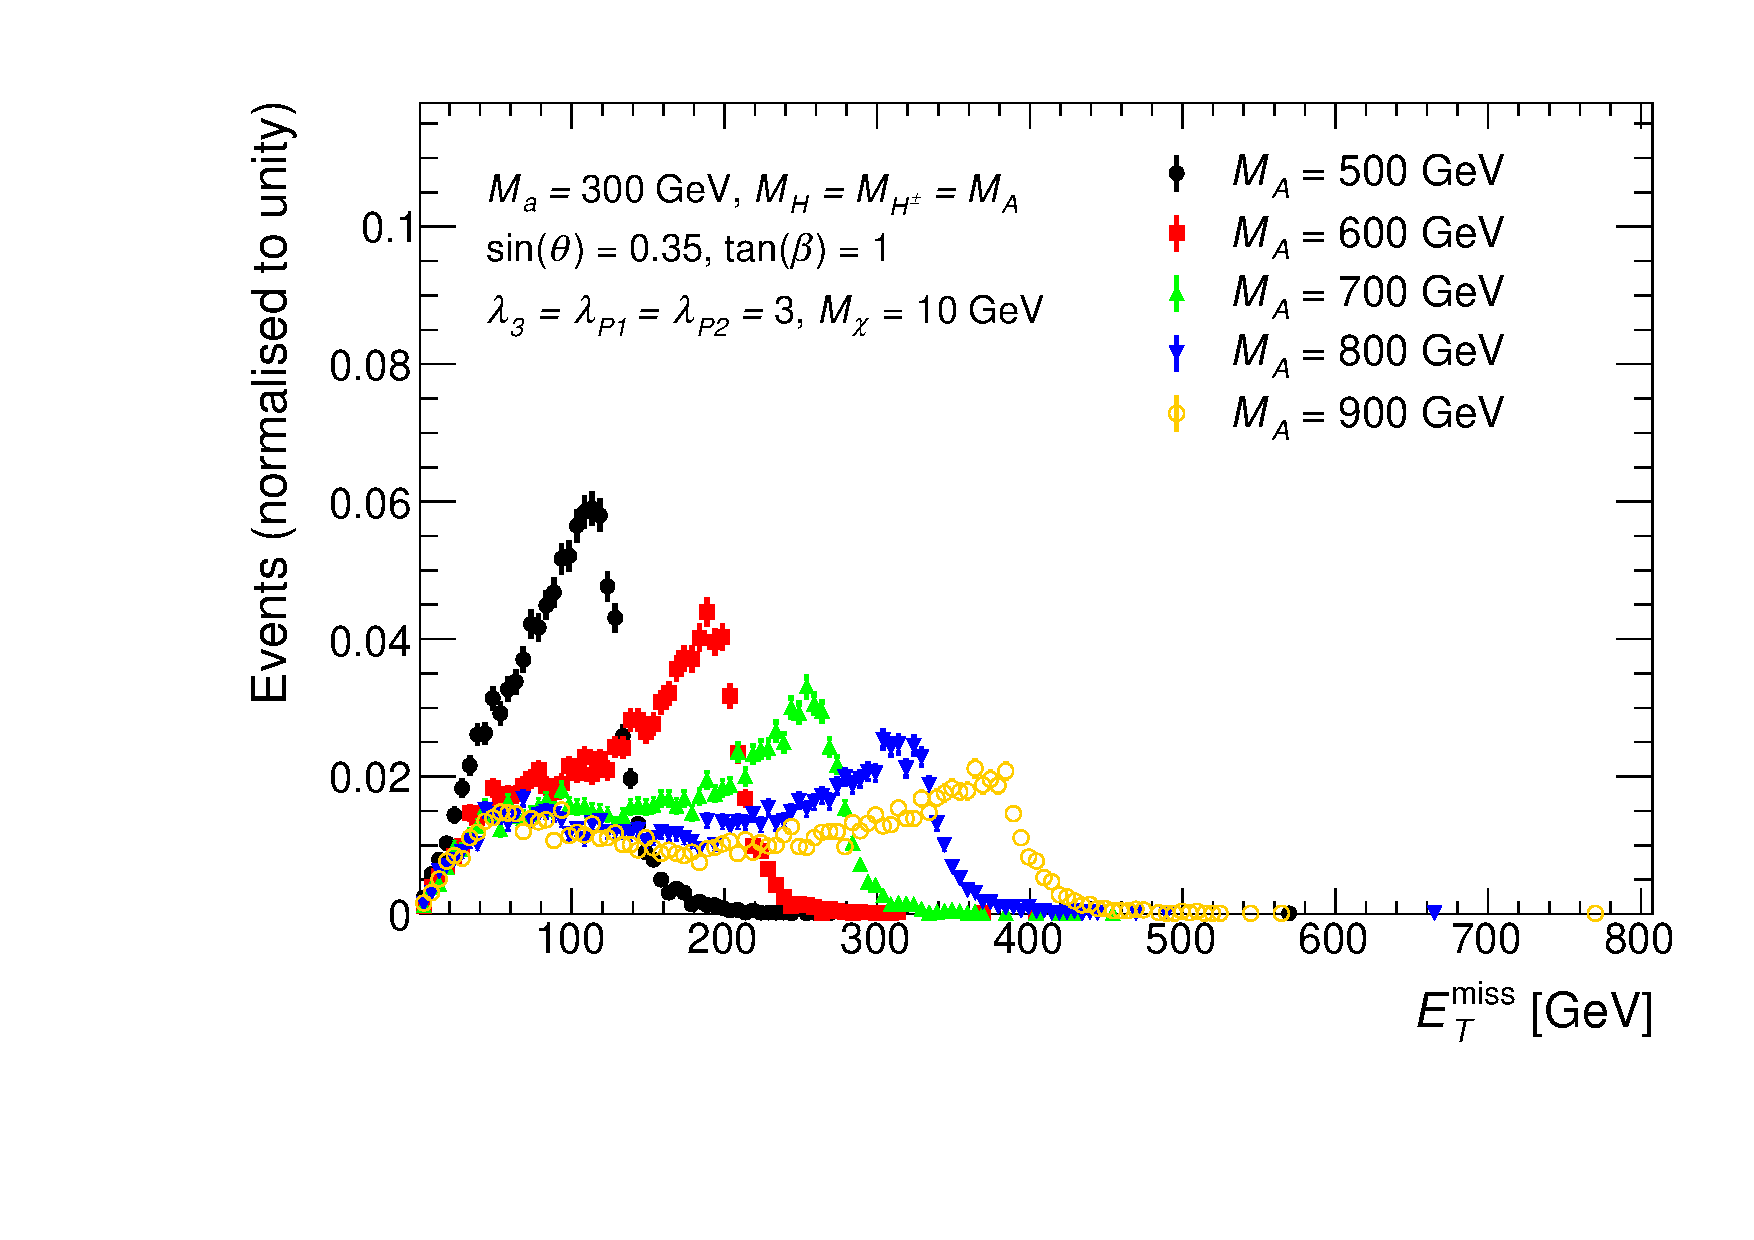
\includegraphics[width=\textwidth]{texinputs/04_grid/figures/monoHbb_m_large_A_scan_MET_liny_norm2one.pdf}
	\caption{$\MET$ distribution for points with different $\mA$
    and fixed $\ma = 300$ GeV. 
	\label{fig:monoHbb_mA_scan_met}} 
    \end{subfigure}
    \begin{subfigure}[t]{0.45\textwidth}
	\centering
	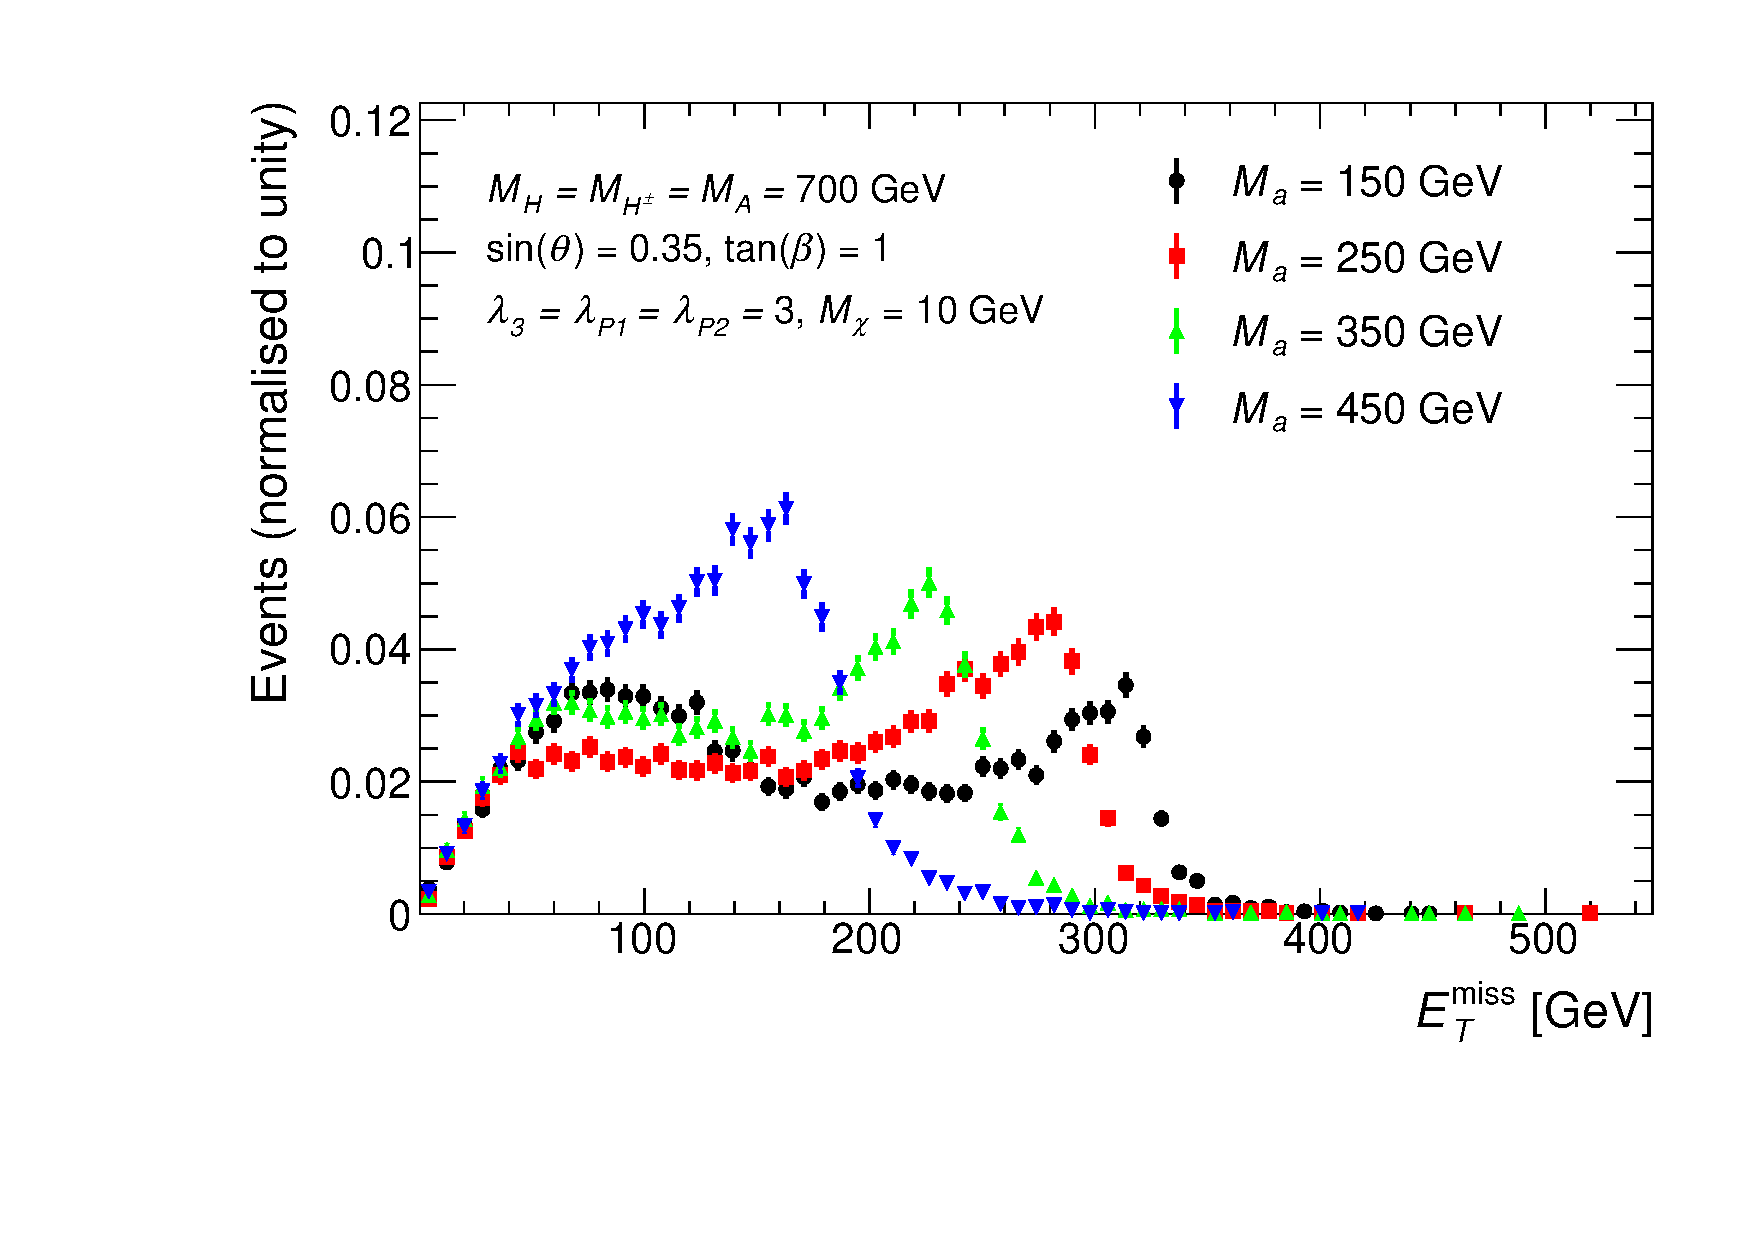
\includegraphics[width=\textwidth]{texinputs/04_grid/figures/monoHbb_m_small_a_scan_MET_liny_norm2one.pdf}	
	\caption{$\MET$ distribution for points with different $\ma$ and fixed $ \mA= 700$ GeV. \label{fig:monoHbb_ma_scan_met}}
    \end{subfigure}
    
    \caption{Parton-level $\MET$ distribution of mono-Higgs events for different $\ma$ and $\mA$, with $\mH = \mHc = \mA$, $ \sinp = 0.35, \tanb = 1, \mDM = 10$ GeV and $ \lap1 = \lap2 = \lam3 = 3 $}
\end{figure}

\begin{figure}%[!htbp]
	\centering

%    \begin{subfigure}[t]{0.7\textwidth}
	\centering
	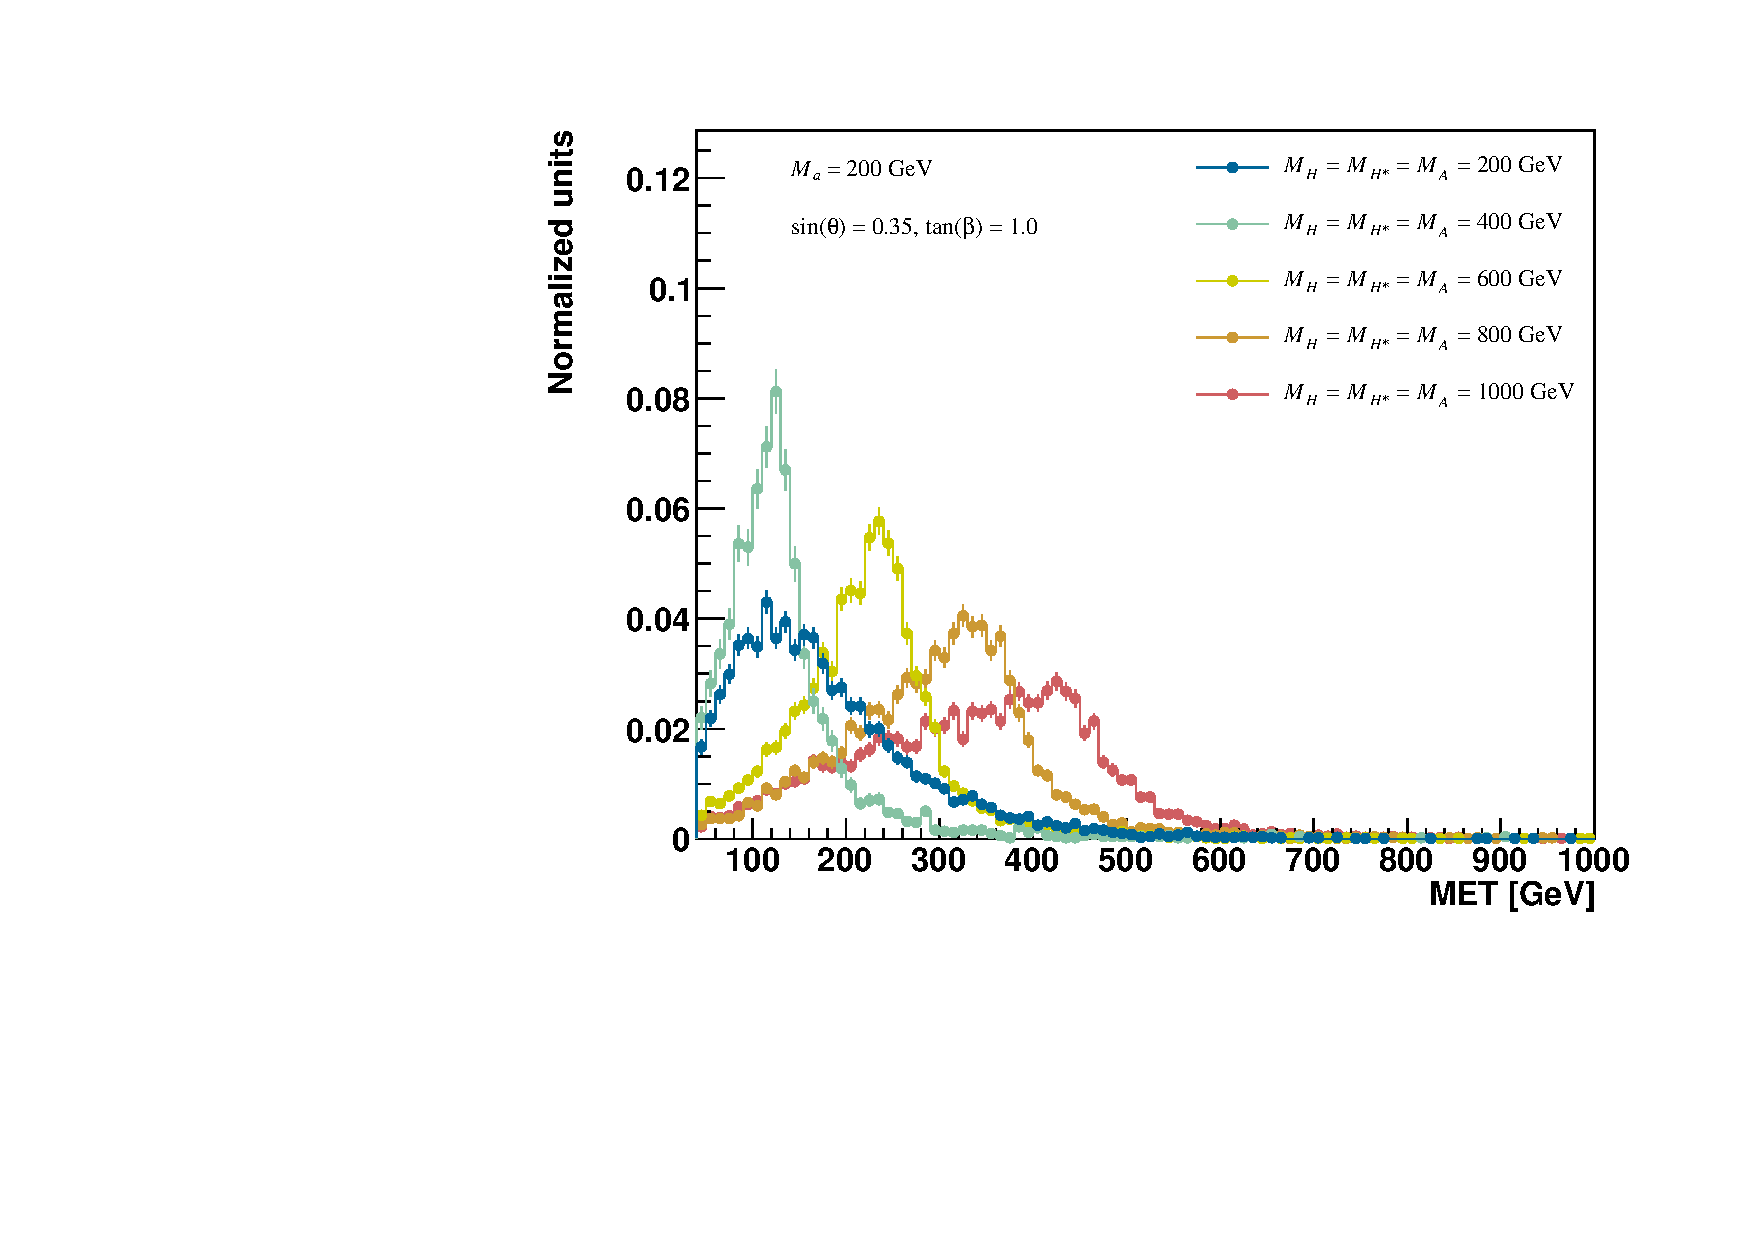
\includegraphics[width=0.7\textwidth]{texinputs/04_grid/figures/monoz/leptonic/mAscan_for_ma200_axis.pdf}	
	\caption{The \MET distribution in signatures including a Z boson after preselection in the leptonic channel, with varying \mH values for fixed $\ma = 200$ GeV and $\mA = \mHc = \mH$. \label{fig:monoz_ll_mA_scan}}
%    \end{subfigure}

\end{figure}

\begin{figure}
\centering

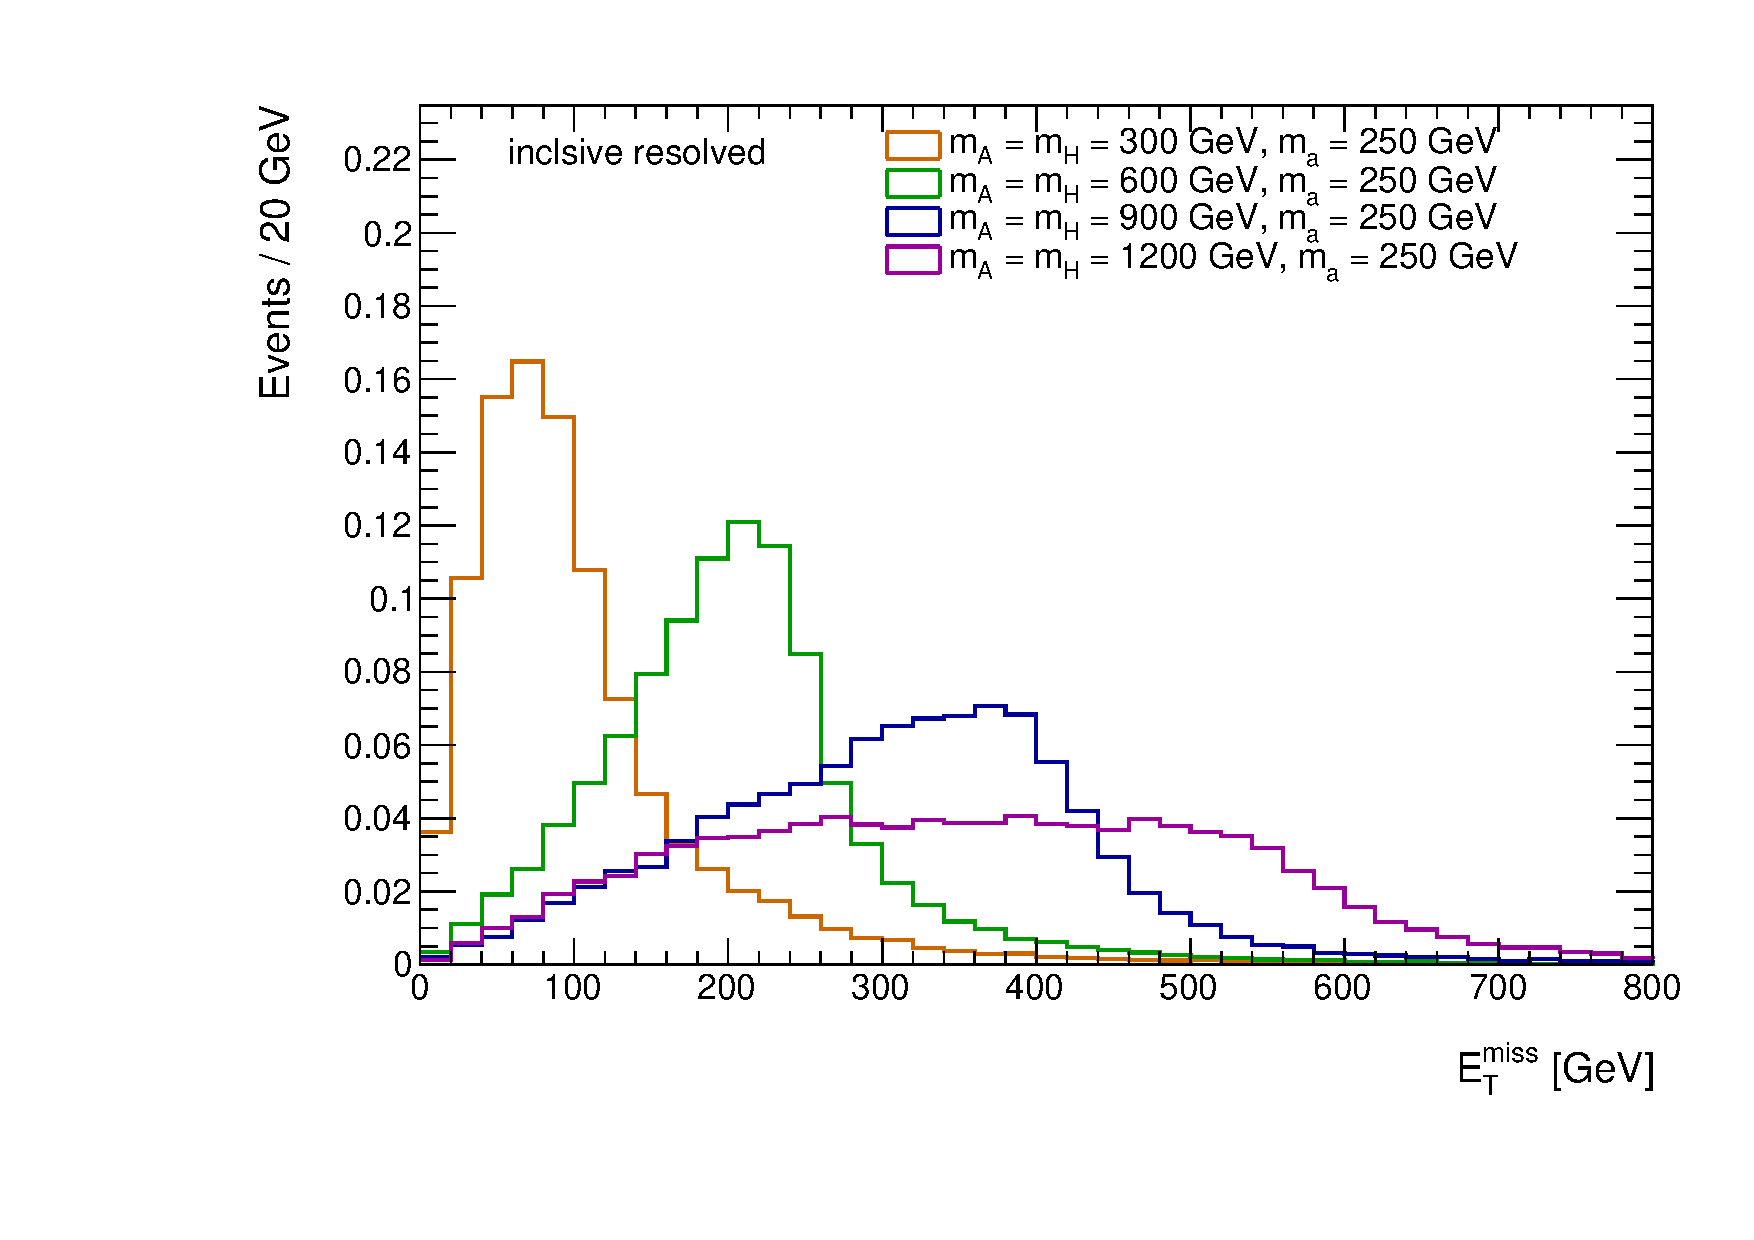
\includegraphics[width=0.45\textwidth]{texinputs/04_grid/figures/monoz/hadronic/ma250_incl_resl_MET_linear.pdf}
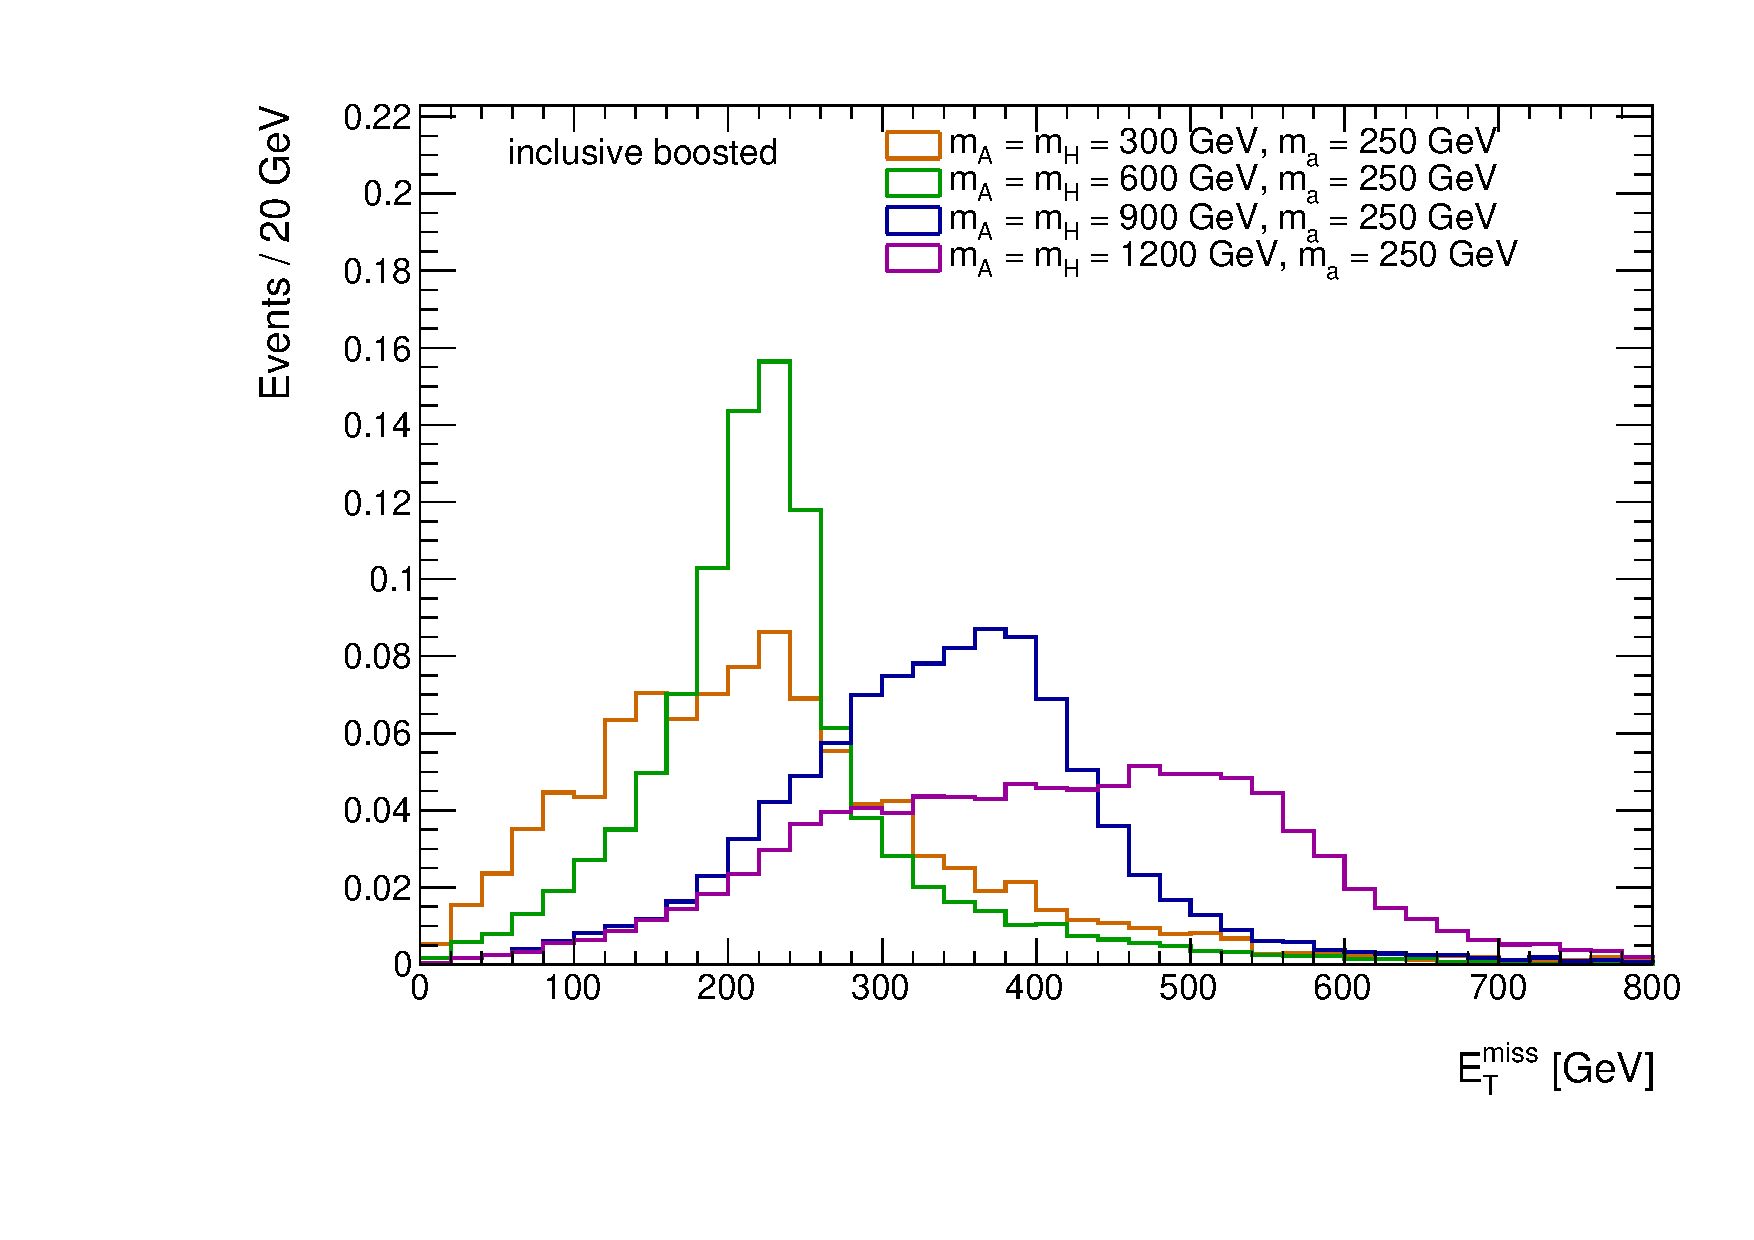
\includegraphics[width=0.45\textwidth]{texinputs/04_grid/figures/monoz/hadronic/ma250_incl_merged_MET_linear.pdf}
\caption{$\MET$ distributions in the resolved (left) and boosted (right) hadronic Z search, after applying the inclusive selection. 
The signal masses are chosen to be $\mH = 300, 600, 900$ and $1200$~GeV with the fixed $\ma = 250$~GeV and $\mA = \mHc = \mH$.
\label{fig:monozhad_kin_inc_fixed_ma}}

\end{figure}

\begin{figure}
\centering

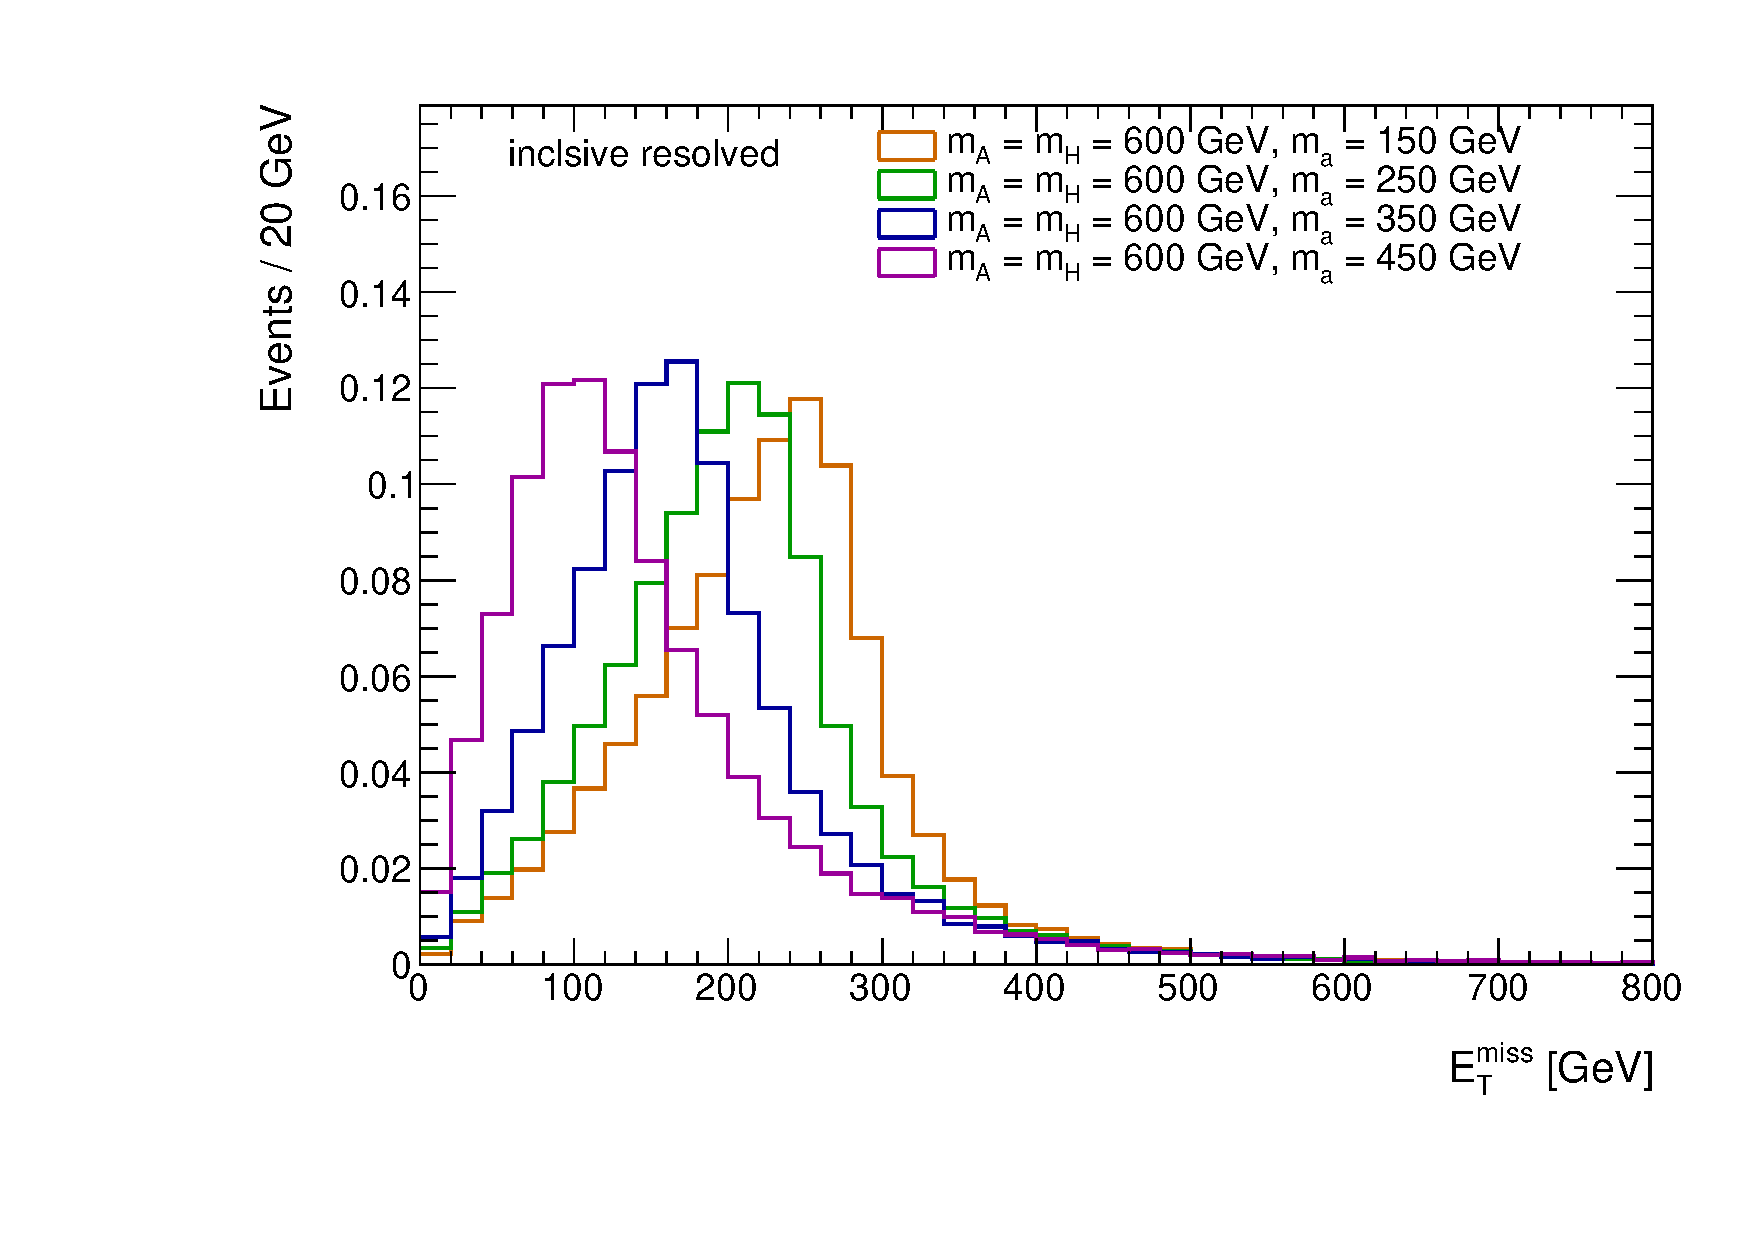
\includegraphics[width=0.45\textwidth]{texinputs/04_grid/figures/monoz/hadronic/mA600_incl_resl_MET_linear.pdf}
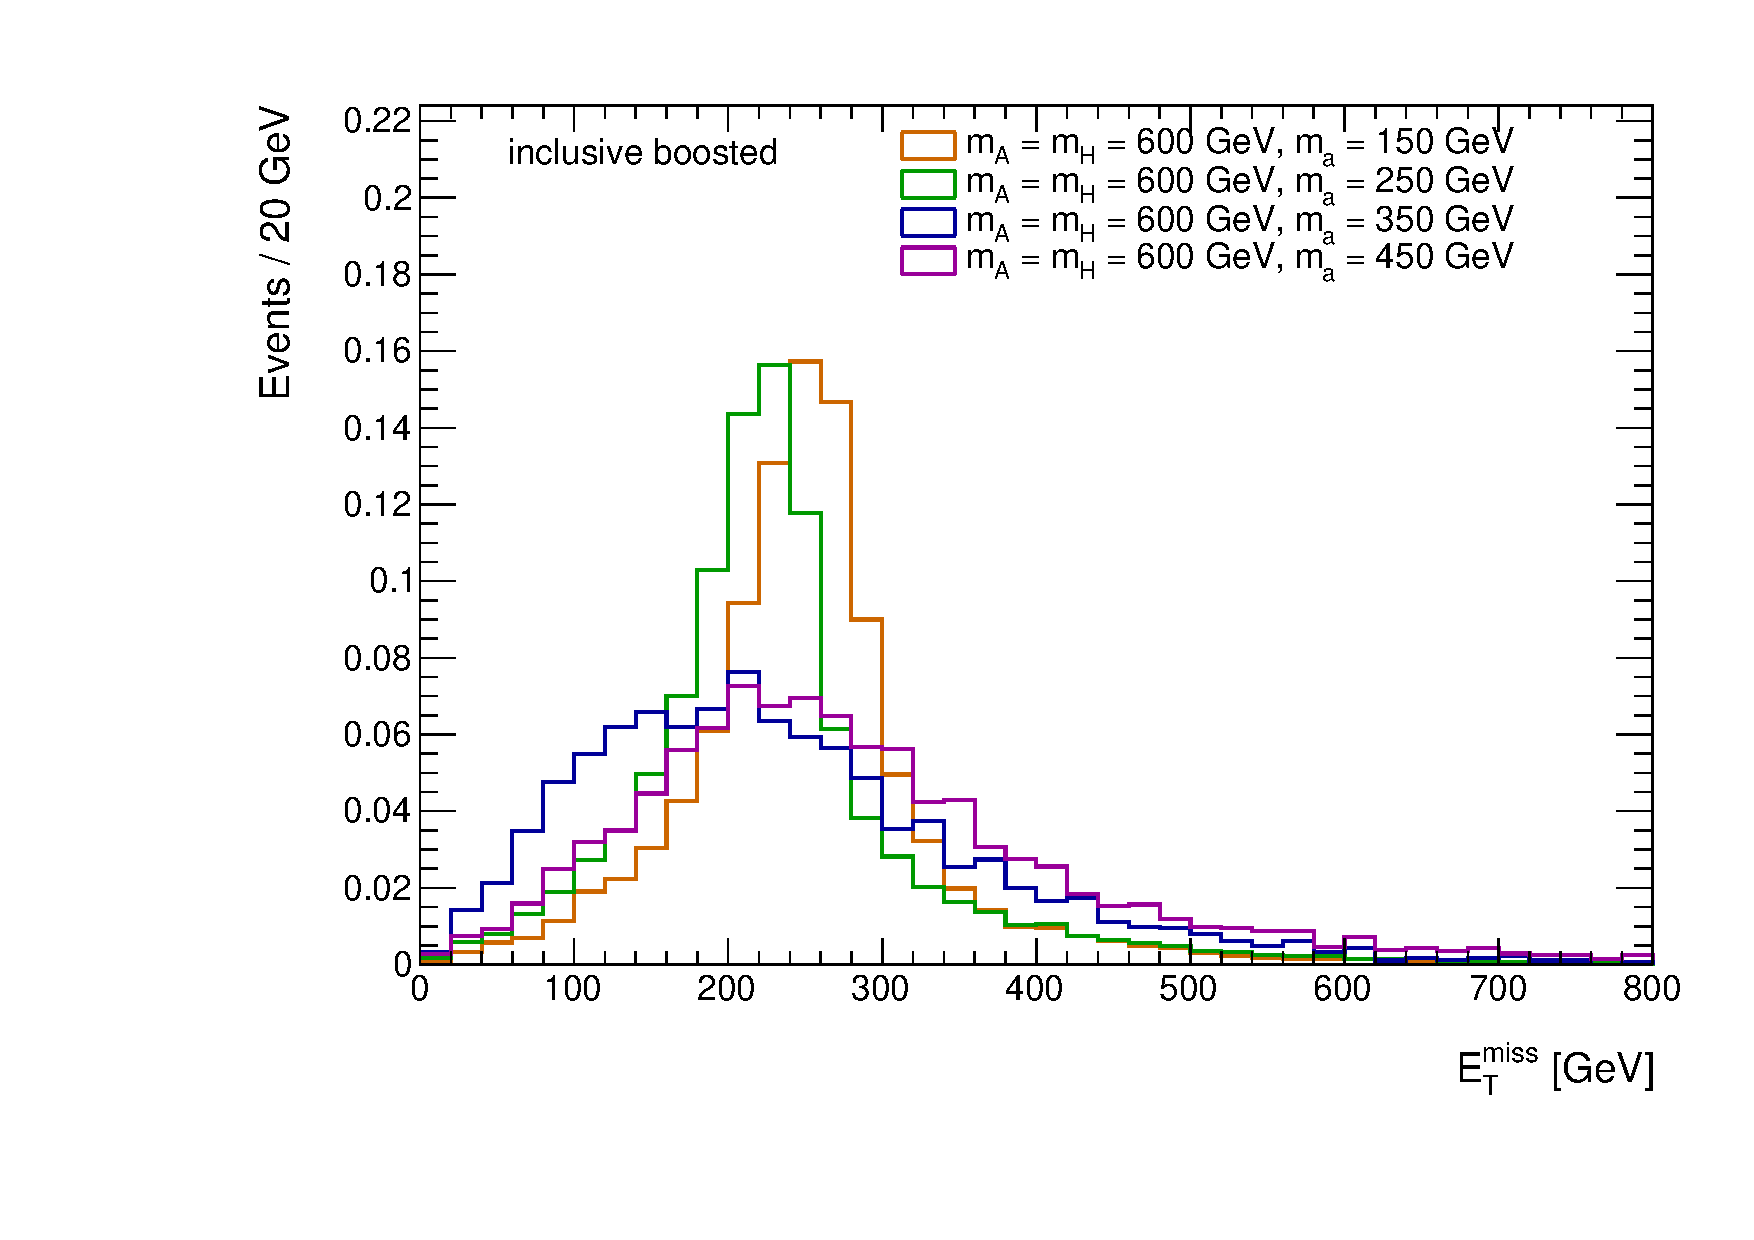
\includegraphics[width=0.45\textwidth]{texinputs/04_grid/figures/monoz/hadronic/mA600_incl_merged_MET_linear.pdf}
\caption{$\MET$ distributions in the resolved (left) and boosted (right) hadronic Z search, after applying the inclusive selection. 
The signal masses are chosen to be $\ma = 150, 250, 350 and 450$~GeV with the fixed $\mH = 600$~GeV ($= \mA = \mHc$).
\label{fig:monozhad_kin_inc_fixed_mA}}

\end{figure}
%Lars: sintheta = 0.35, tanbeta = 1, mDM = 10 etc.? Would be good to have in caption/on plot

A potentially large fraction of the mono-$h$ signal events is also produced in non-resonant $2 \to 3$ processes $gg \to h \chi \chi$, as in \autoref{fig:feyn_hdm_box}, leading to a broader distribution of the invariant mass of the decay products. 
%link into thereory section graph or cite paper
Consequently, this results in a broader and softer \met distribution that is distinct from the Jacobian peak discussed above, 
and contributes to the off-peak features of \autoref{fig:monoHbb_ma_scan_met} and \autoref{fig:monoHbb_mA_scan_met}. 

The masses \ma and \mA influence the kinematics in the $t\bar{t}$ + \MET signature as well. As shown in \autoref{fig:kin_Ma}, the $E_{T}^{miss}$, and leading and trailing top quark $p_{T}$ distributions broaden with increasing $\mathrm{M_{a}}$. 
Similarly, for values of $\mathrm{M_{A}} < \mathrm{M_{a}}$, as $\mathrm{M_{A}}$ increases, the kinematic distributions mentioned above also broaden, as shown in \autoref{fig:kin_MA}.

\begin{figure}
  \centering
  
  \begin{subfigure}[b]{0.7\textwidth}
    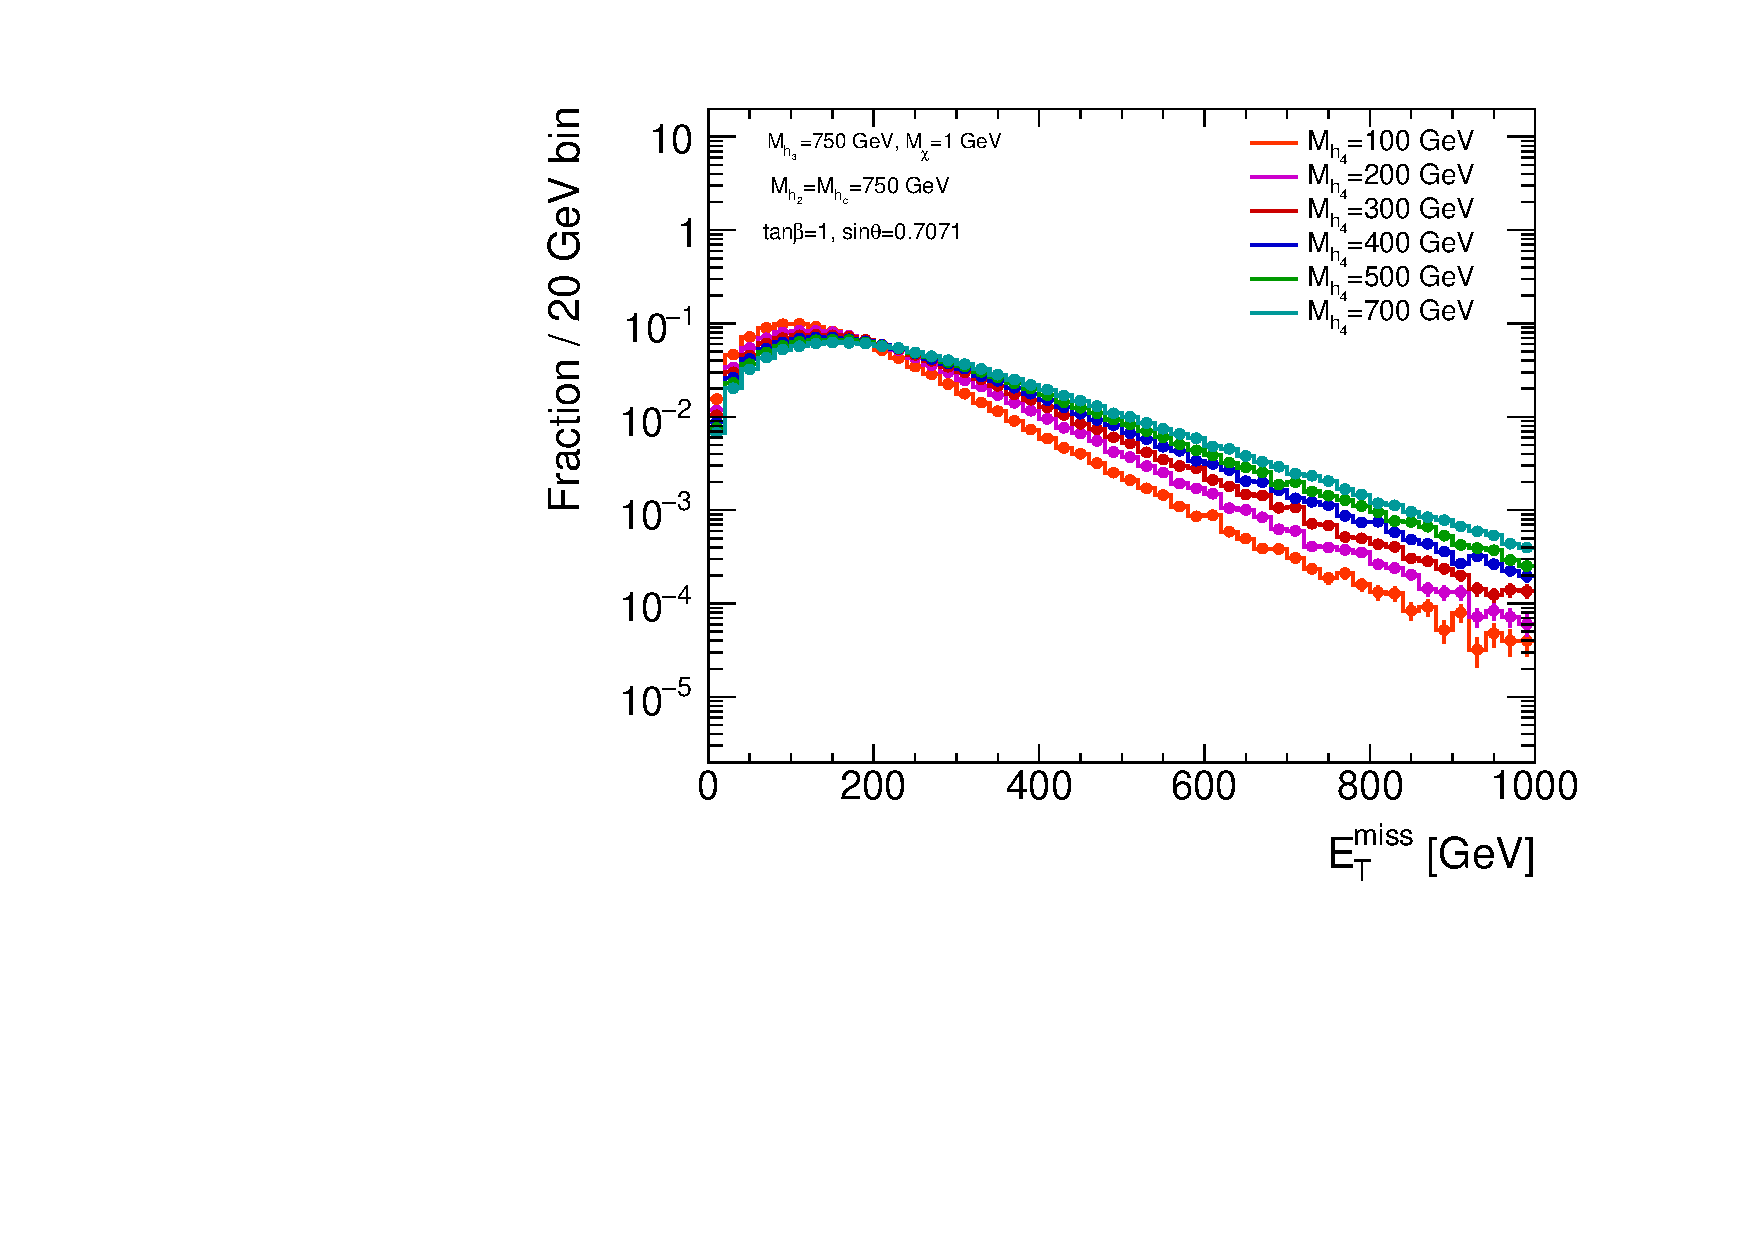
\includegraphics[width=\textwidth]{texinputs/04_grid/figures/DMHF/benchmarking/MDM_1_MA_750_sinp_0.7071_tanb_1.0_SCAN_Ma/metlog.pdf}
    \caption{$E_{T}^{miss}$}
  \end{subfigure}\\
  
  \begin{subfigure}[b]{0.45\textwidth}
    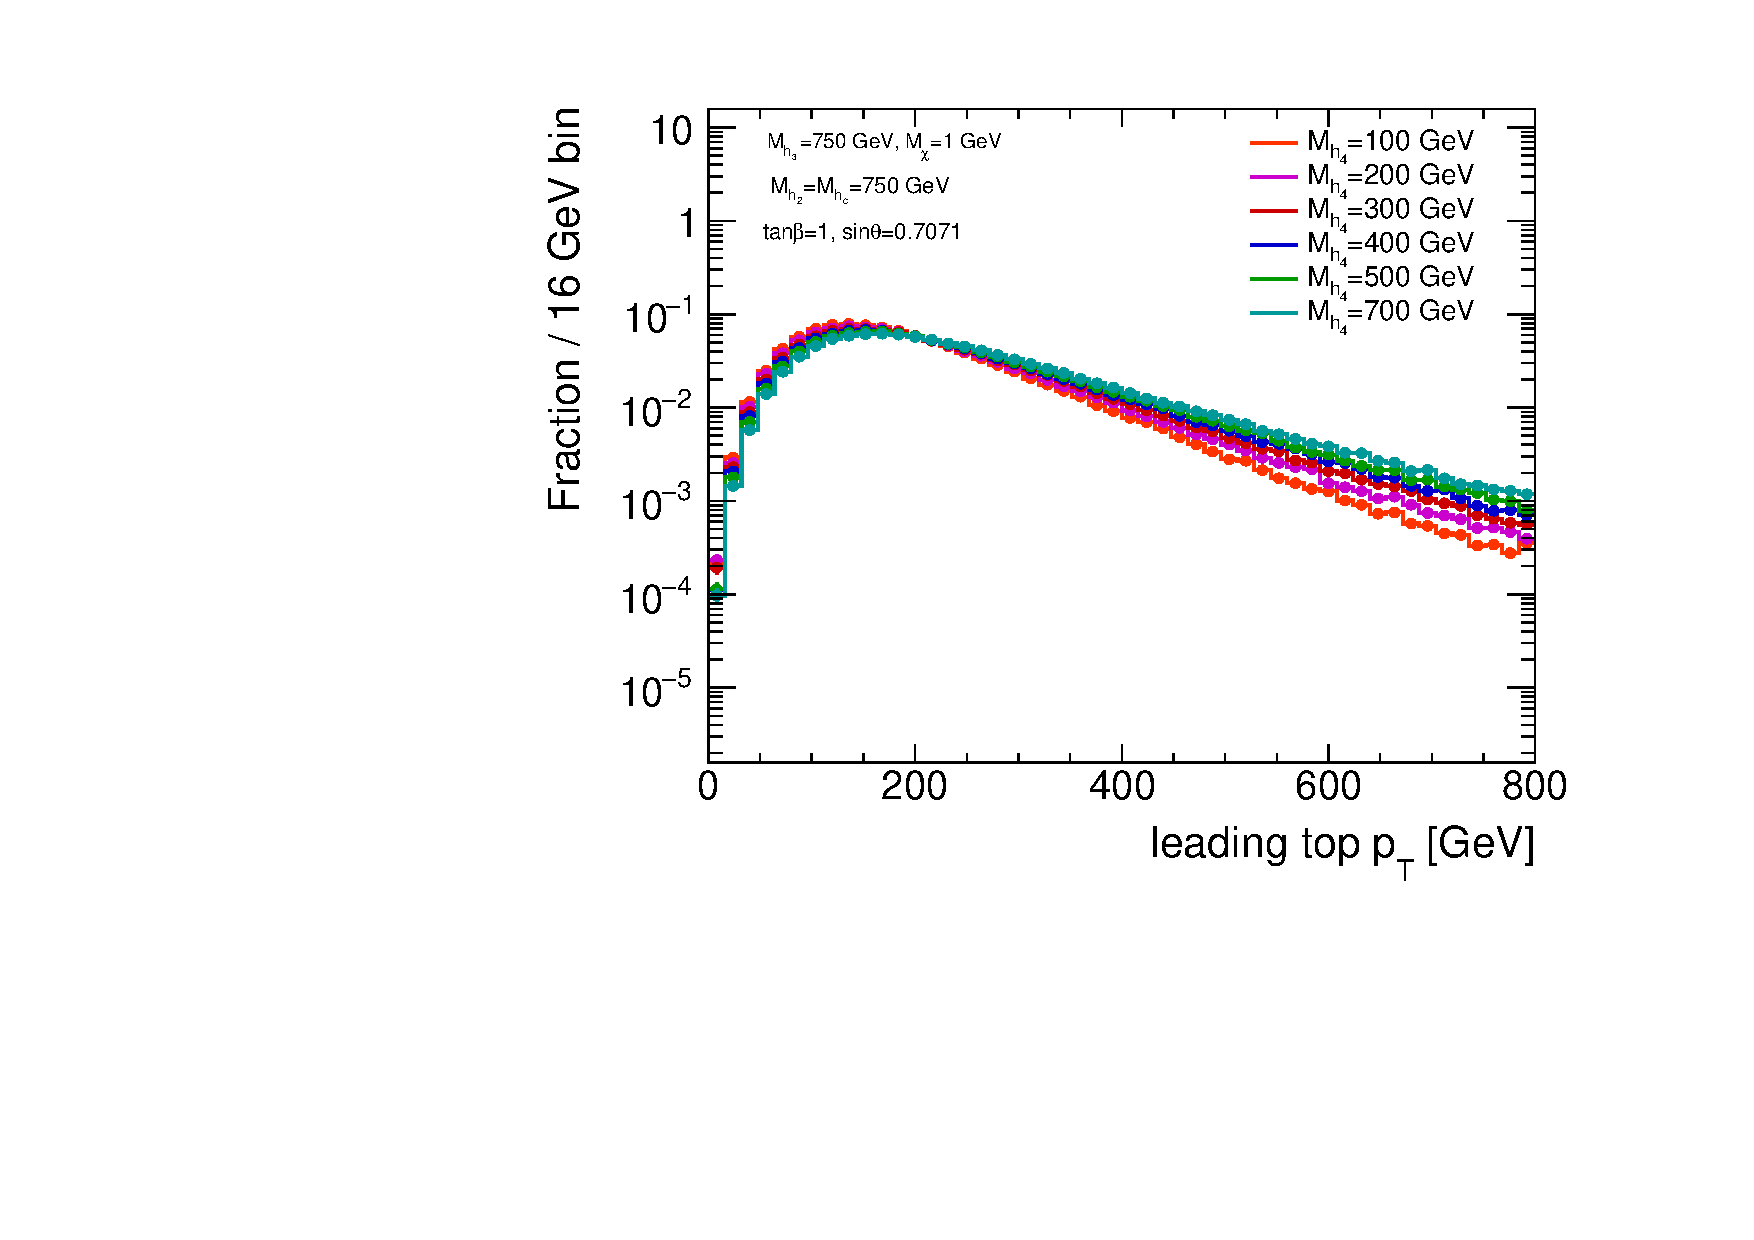
\includegraphics[width=\textwidth]{texinputs/04_grid/figures/DMHF/benchmarking/MDM_1_MA_750_sinp_0.7071_tanb_1.0_SCAN_Ma/top1ptlog.pdf}
    \caption{Leading top quark $p_{T}$}
  \end{subfigure} 
  \begin{subfigure}[b]{0.45\textwidth}
    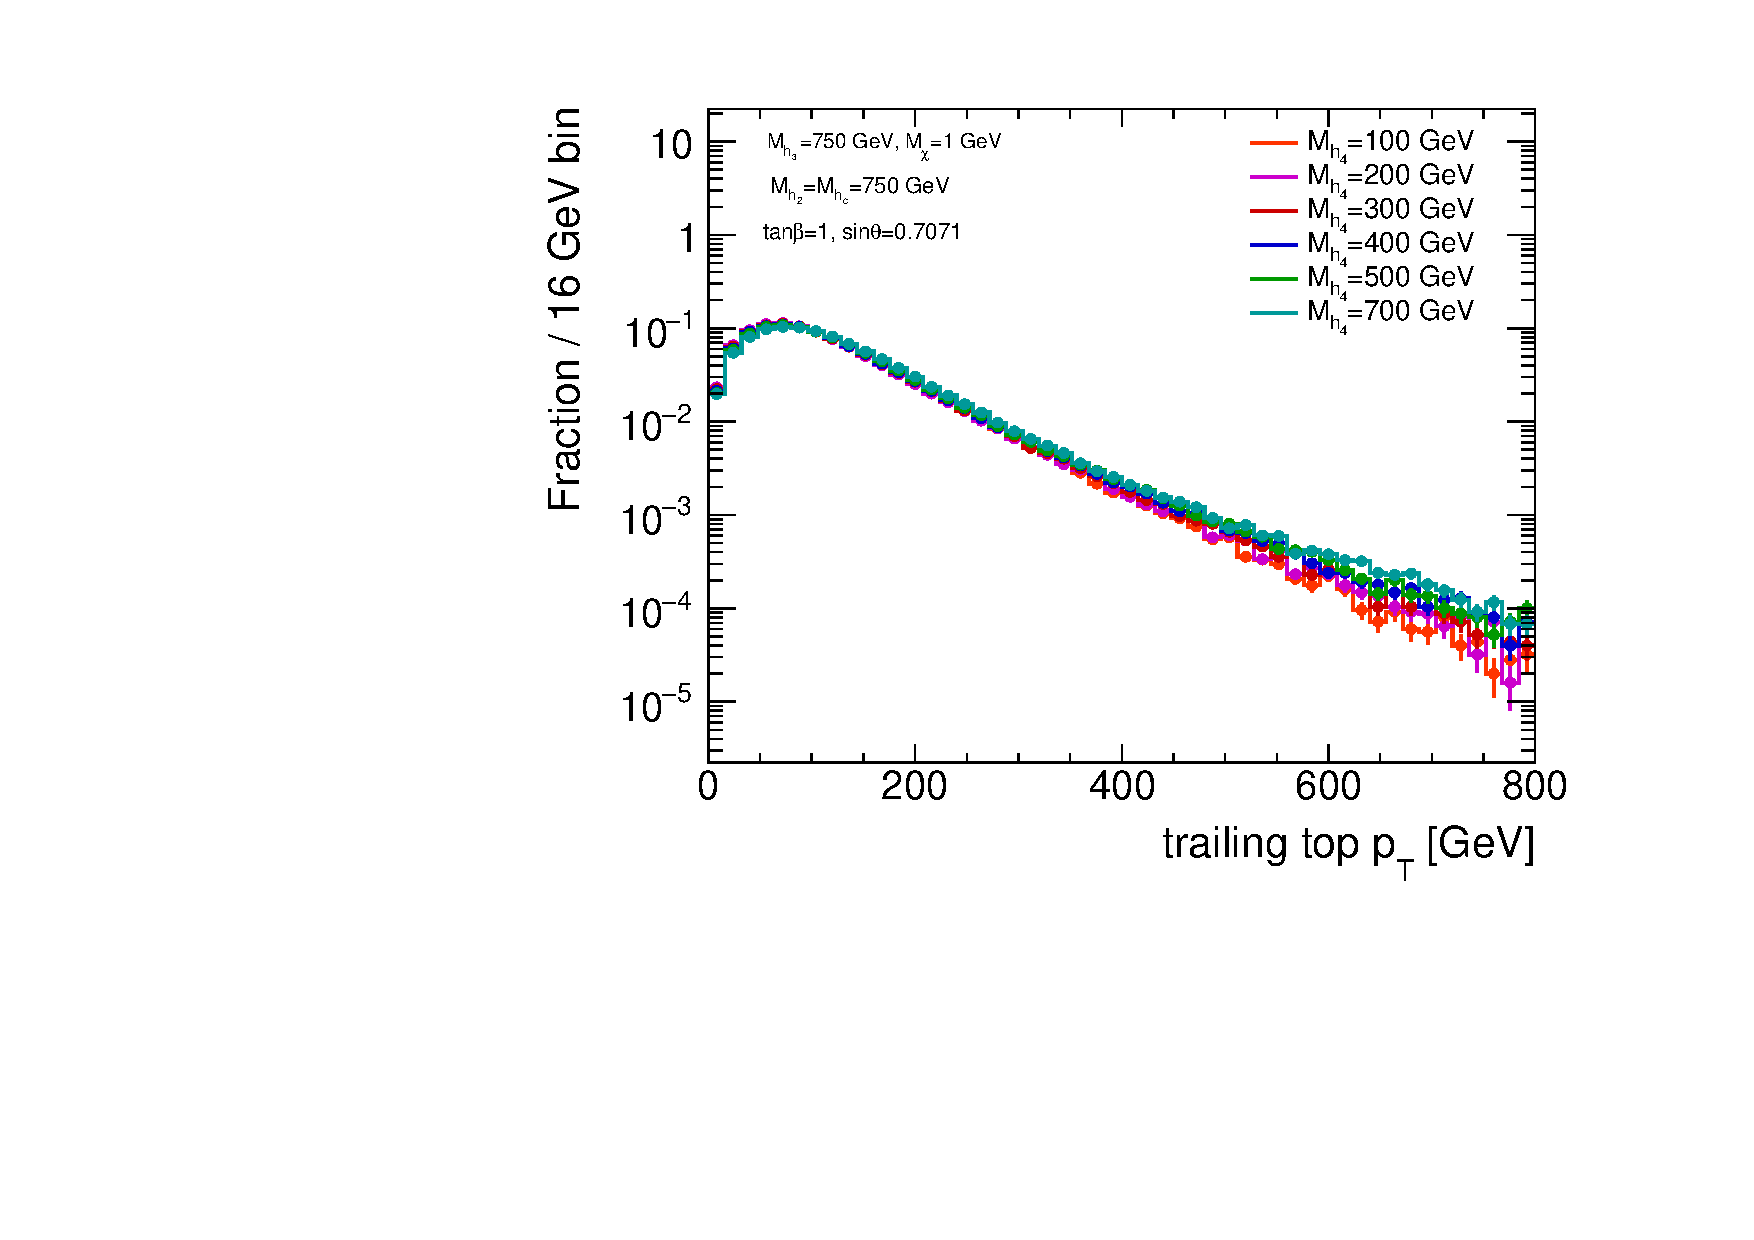
\includegraphics[width=\textwidth]{texinputs/04_grid/figures/DMHF/benchmarking/MDM_1_MA_750_sinp_0.7071_tanb_1.0_SCAN_Ma/top2ptlog.pdf}
    \caption{Trailing top quark $p_{T}$}
  \end{subfigure}
  
  \caption{The $E_{T}^{miss}$, leading and trailing top $p_{T}$ distributions for inclusive $t\bar{t}+\chi\bar{\chi}$ production for various values of $\mathrm{M_a}$, with $\mathrm{M_A}=750$ GeV, $\mathrm{M_H}=\mathrm{M_{H^{\pm}}}=750$ GeV, $\tan\beta=1$, and $\sin\theta=0.7071$.\label{fig:kin_Ma}}
  
\end{figure}

\begin{figure}
  \centering
  
  \begin{subfigure}[b]{0.7\textwidth}
    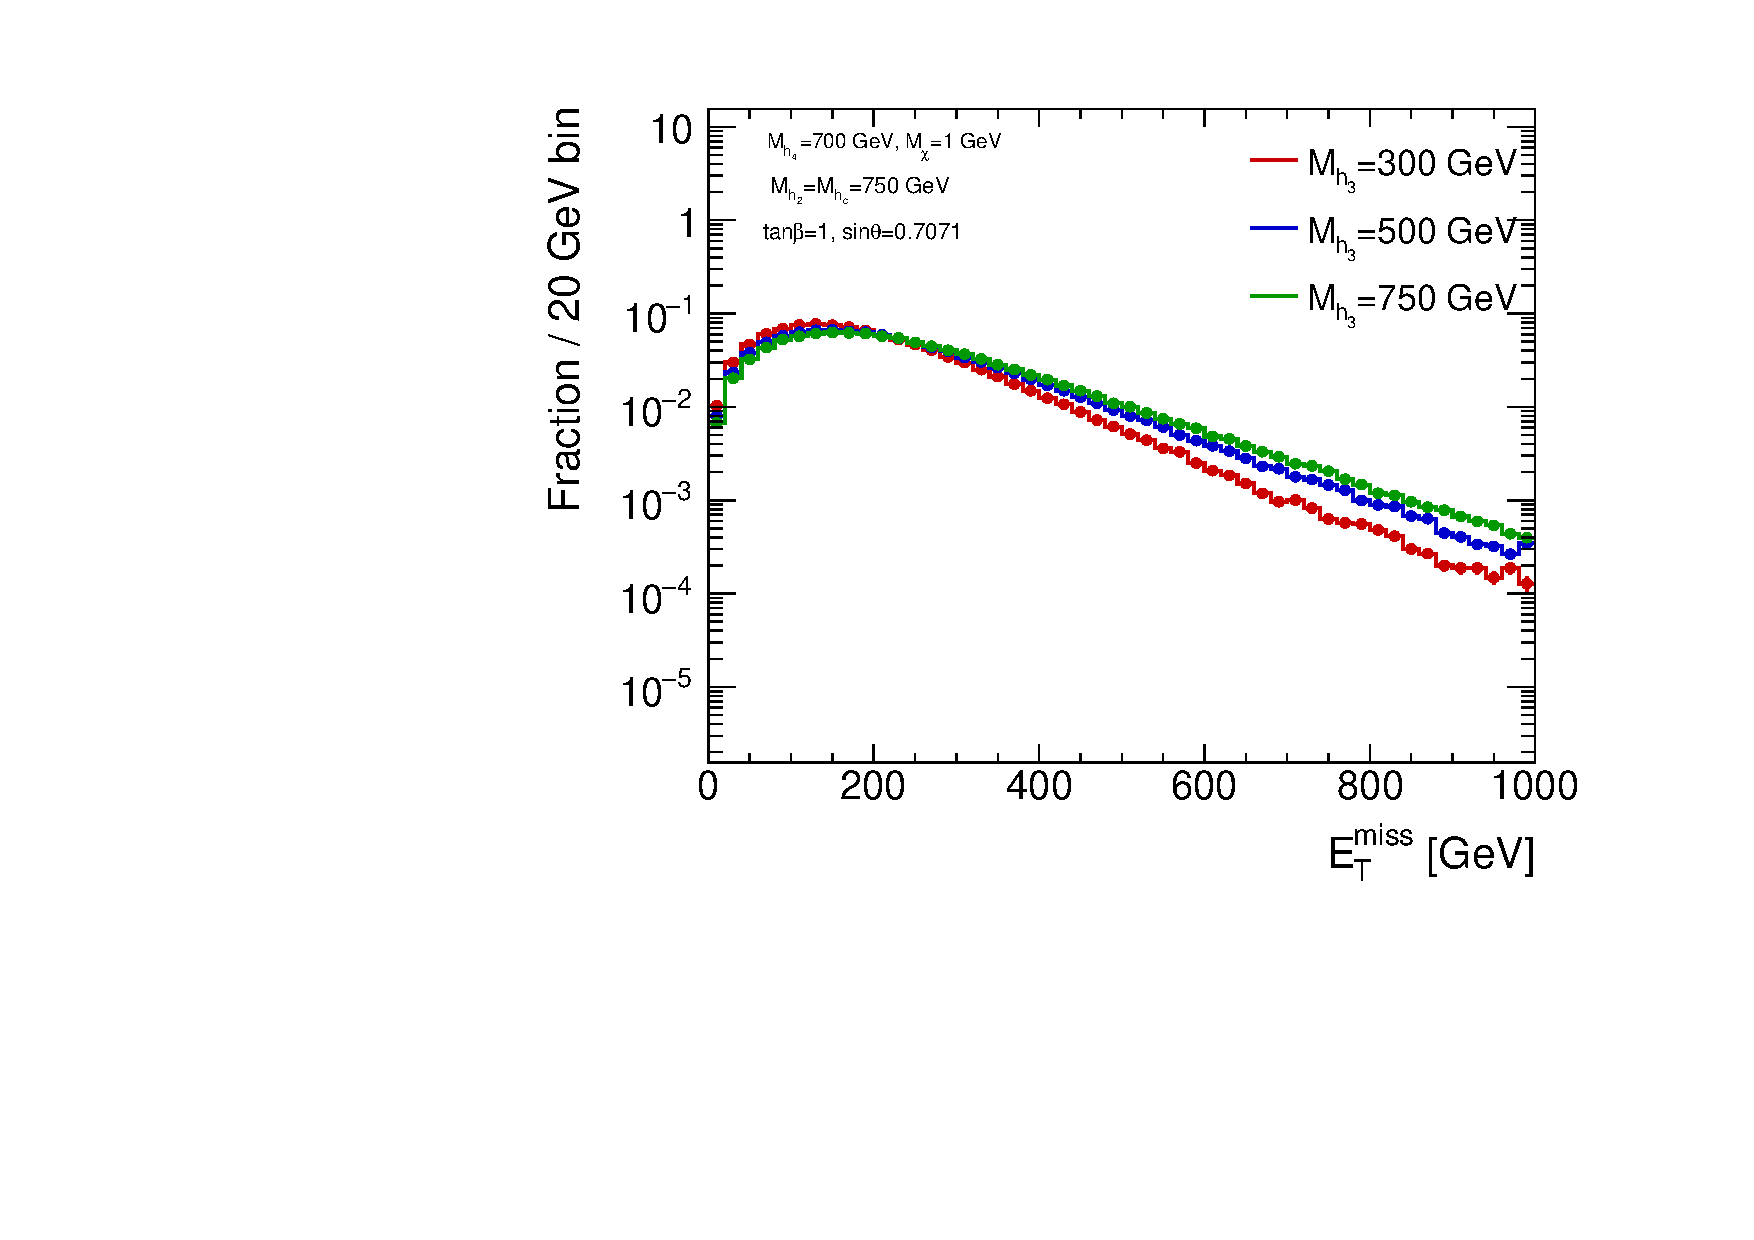
\includegraphics[width=\textwidth]{texinputs/04_grid/figures/DMHF/benchmarking/MDM_1_Ma_700_sinp_0.7071_tanb_1.0_SCAN_MA/metlog.pdf}
    \caption{$E_{T}^{miss}$}
  \end{subfigure}\\
  
  \begin{subfigure}[b]{0.45\textwidth}
    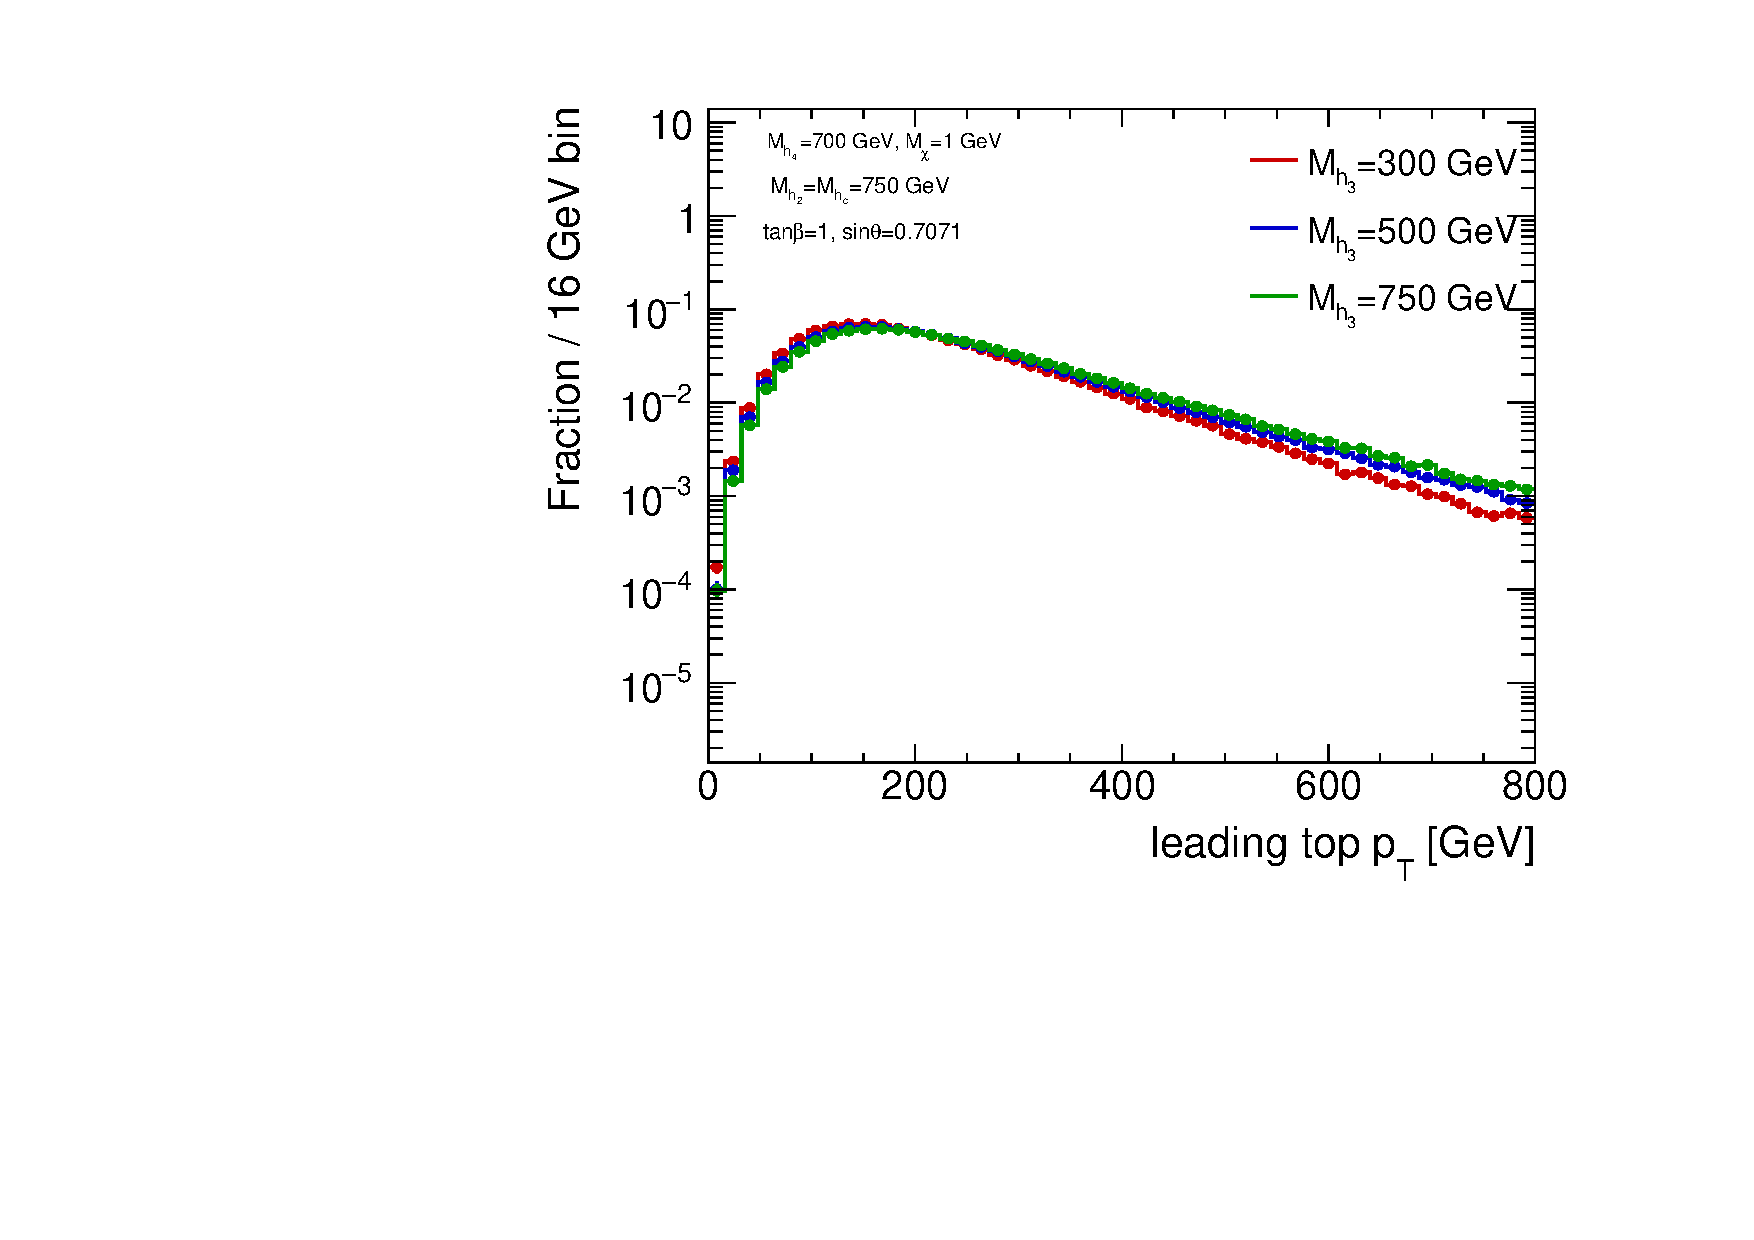
\includegraphics[width=\textwidth]{texinputs/04_grid/figures/DMHF/benchmarking/MDM_1_Ma_700_sinp_0.7071_tanb_1.0_SCAN_MA/top1ptlog.pdf}
    \caption{Leading top $p_{T}$}
  \end{subfigure}
  \begin{subfigure}[b]{0.45\textwidth}
    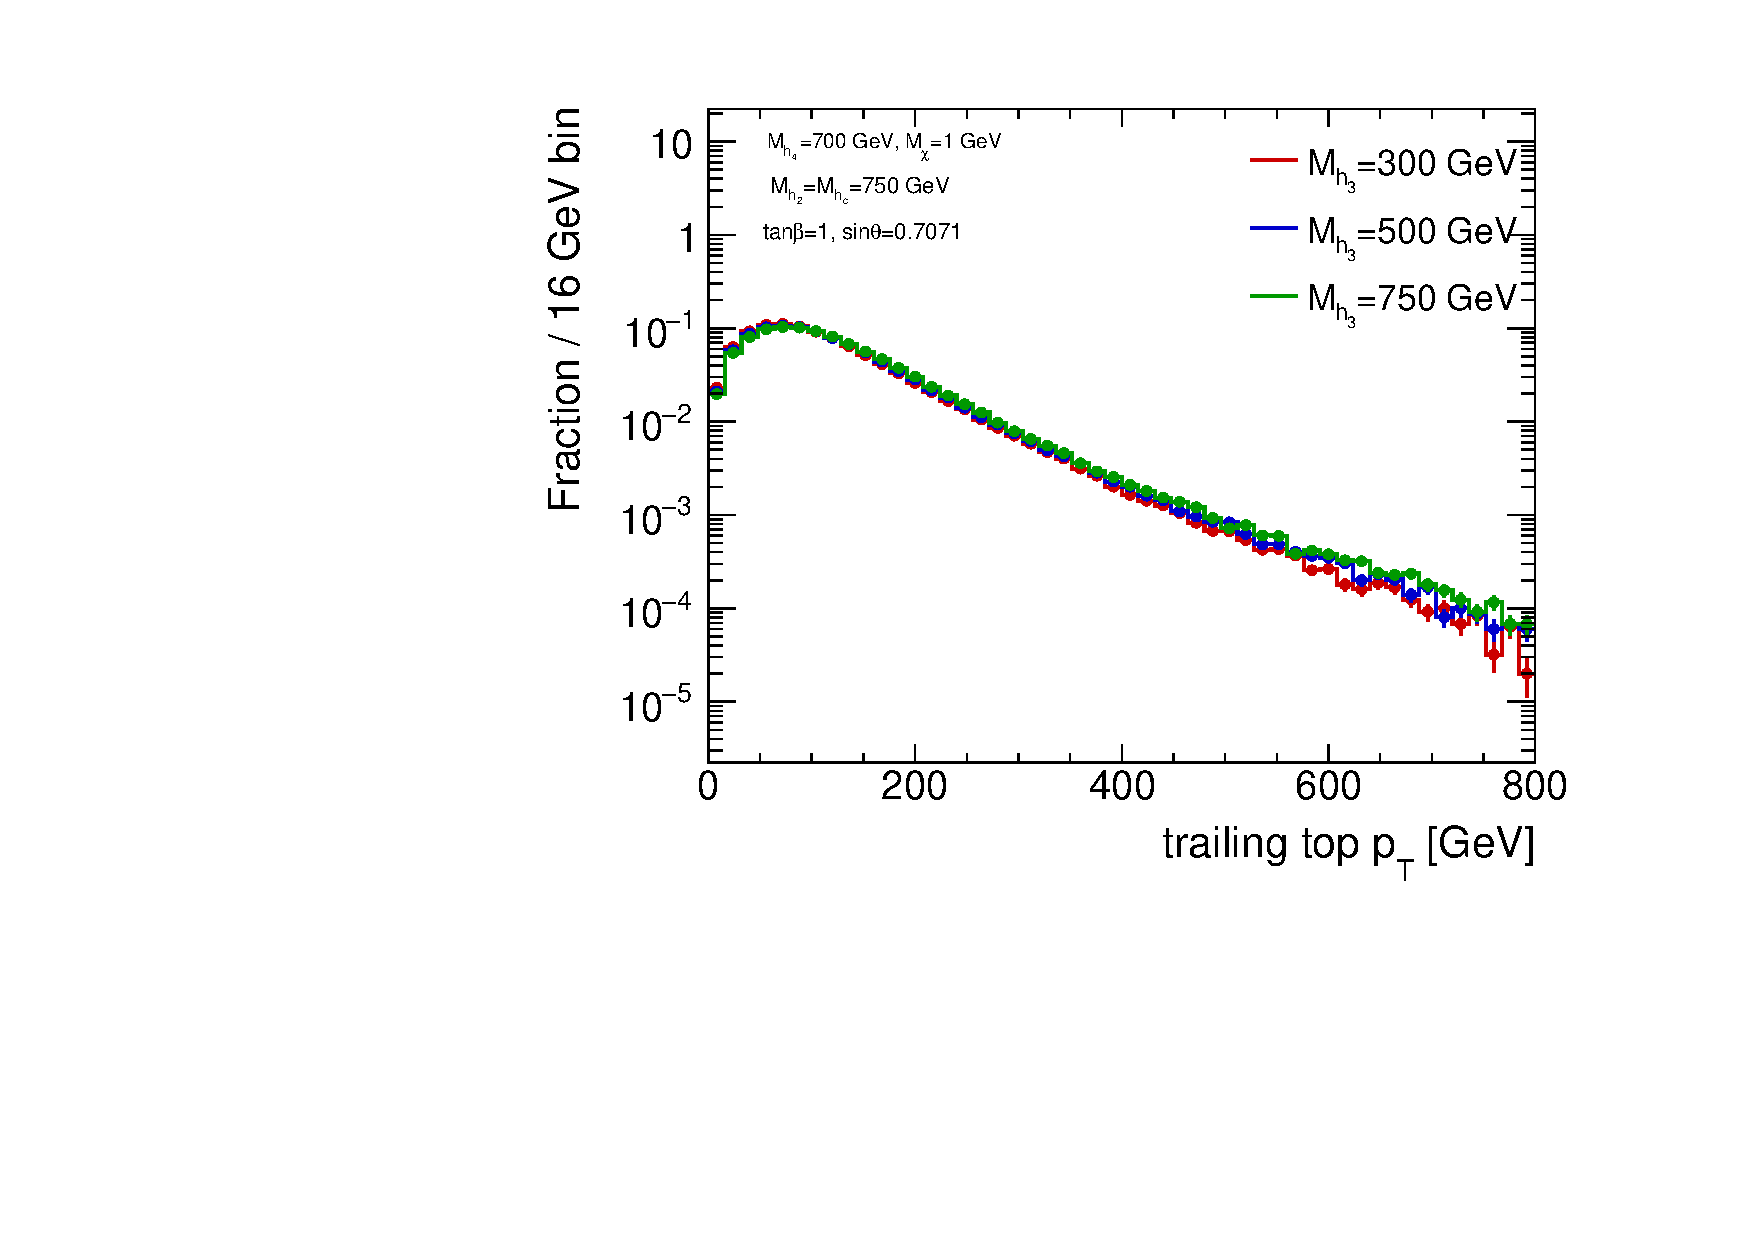
\includegraphics[width=\textwidth]{texinputs/04_grid/figures/DMHF/benchmarking/MDM_1_Ma_700_sinp_0.7071_tanb_1.0_SCAN_MA/top2ptlog.pdf}
    \caption{Trailing top $p_{T}$}
  \end{subfigure}
  
  \caption{The $E_{T}^{miss}$, leading and trailing top $p_{T}$ distributions for inclusive $t\bar{t}+\chi\bar{\chi}$ production for various values of $\mathrm{M_A}$, with $\mathrm{M_a}=700$ GeV, $\mathrm{M_H}=\mathrm{M_{H^{\pm}}}=750$ GeV, $\tan\beta=1$, and $\sin\theta=0.7071$, before any analysis selection.\label{fig:kin_MA}}
 
\end{figure}

Since the shape of the $\MET$ distribution affects the design of experimental searches, and to a large extent their sensitivity, ~\emph{it is desirable to scan the $\mA$ and $\ma$ parameter space}. 

%In conclusion, the $\mA$ and $\ma$ parameters strongly affect the sensitivity of a search for the \hdma model using the \monohbb signature because they determine the location of the Jacobian peak in the \met distribution. Therefore, one of the proposed parameter scans for the \hdma model is in the ($\ma$,$\mA$) plane.

\begin{figure}%[!htpb]
\centering

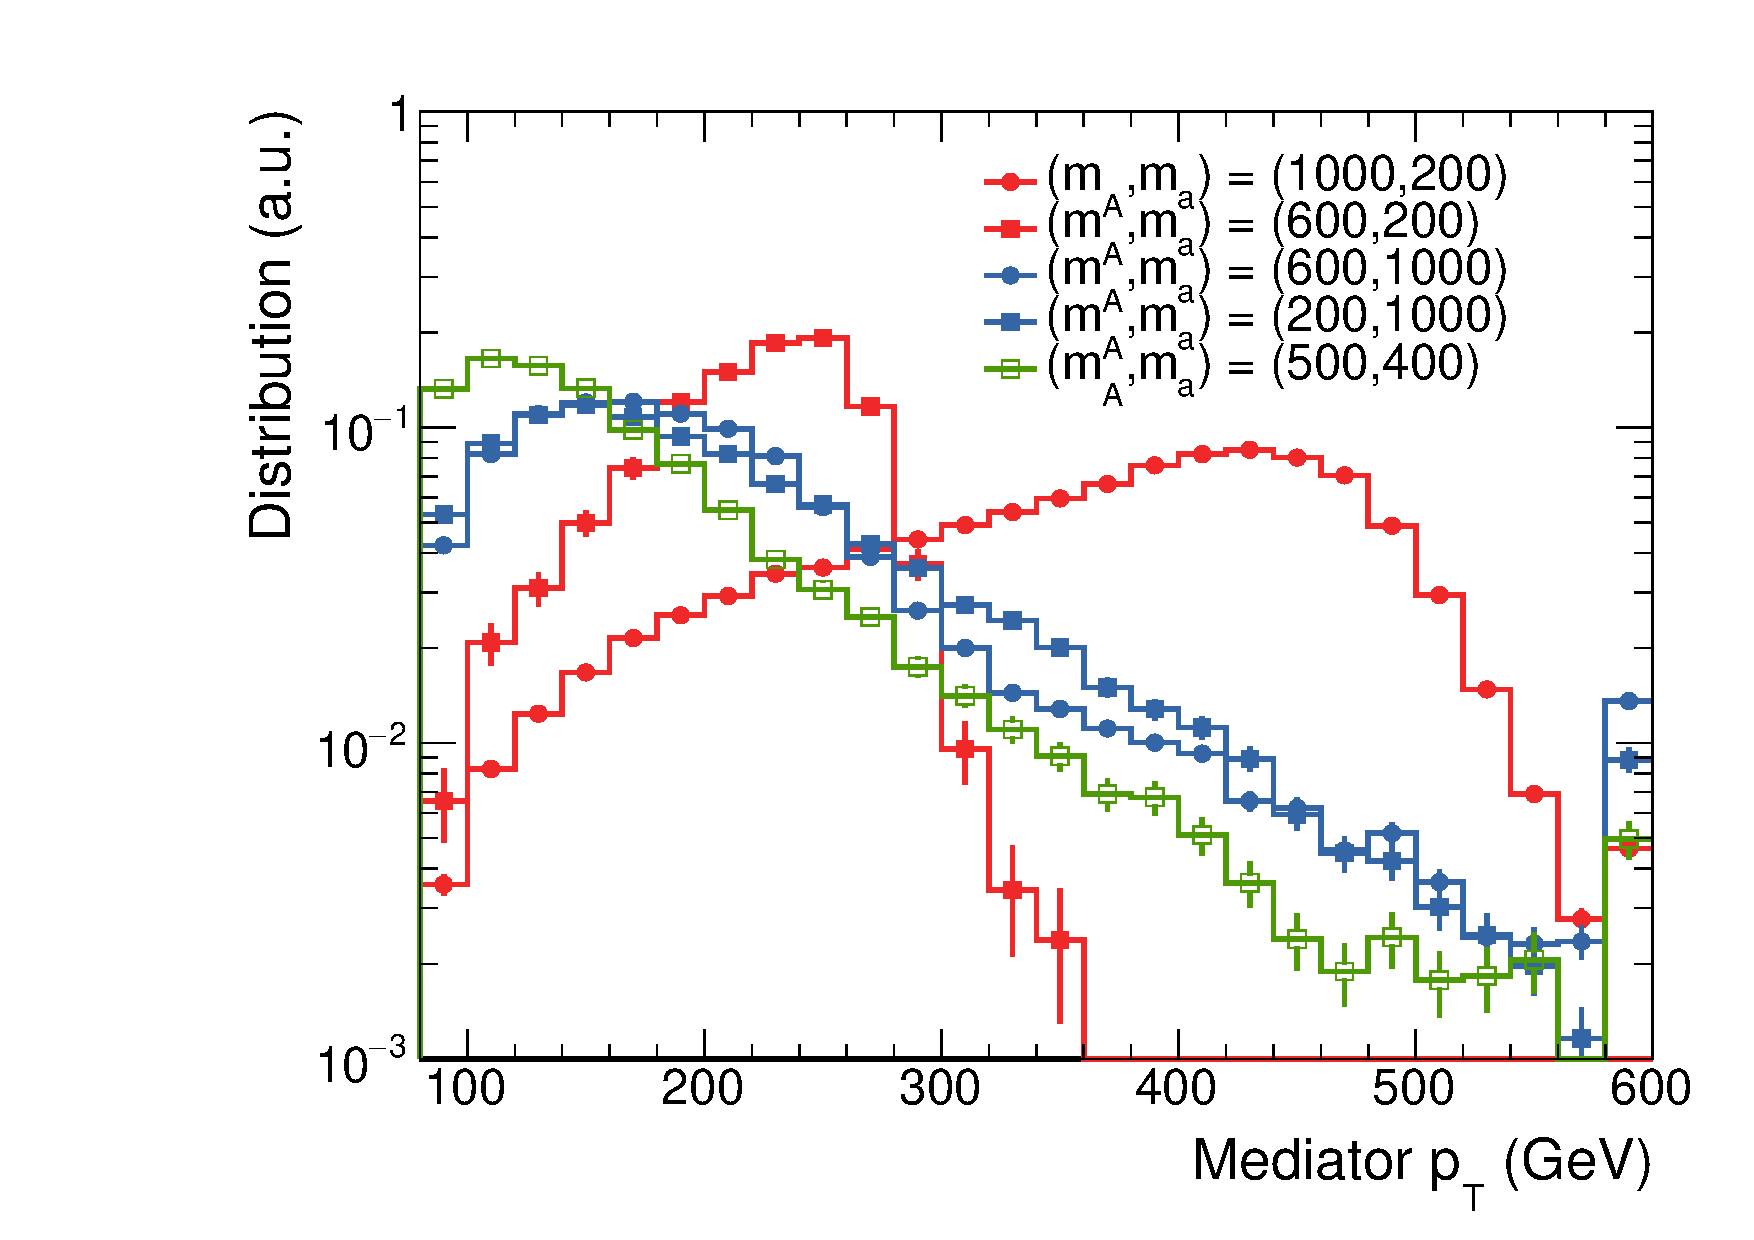
\includegraphics[width=0.45\textwidth]{texinputs/04_grid/figures/monoz/leptonic/dmwg-final_h_pt_med_dm.pdf}
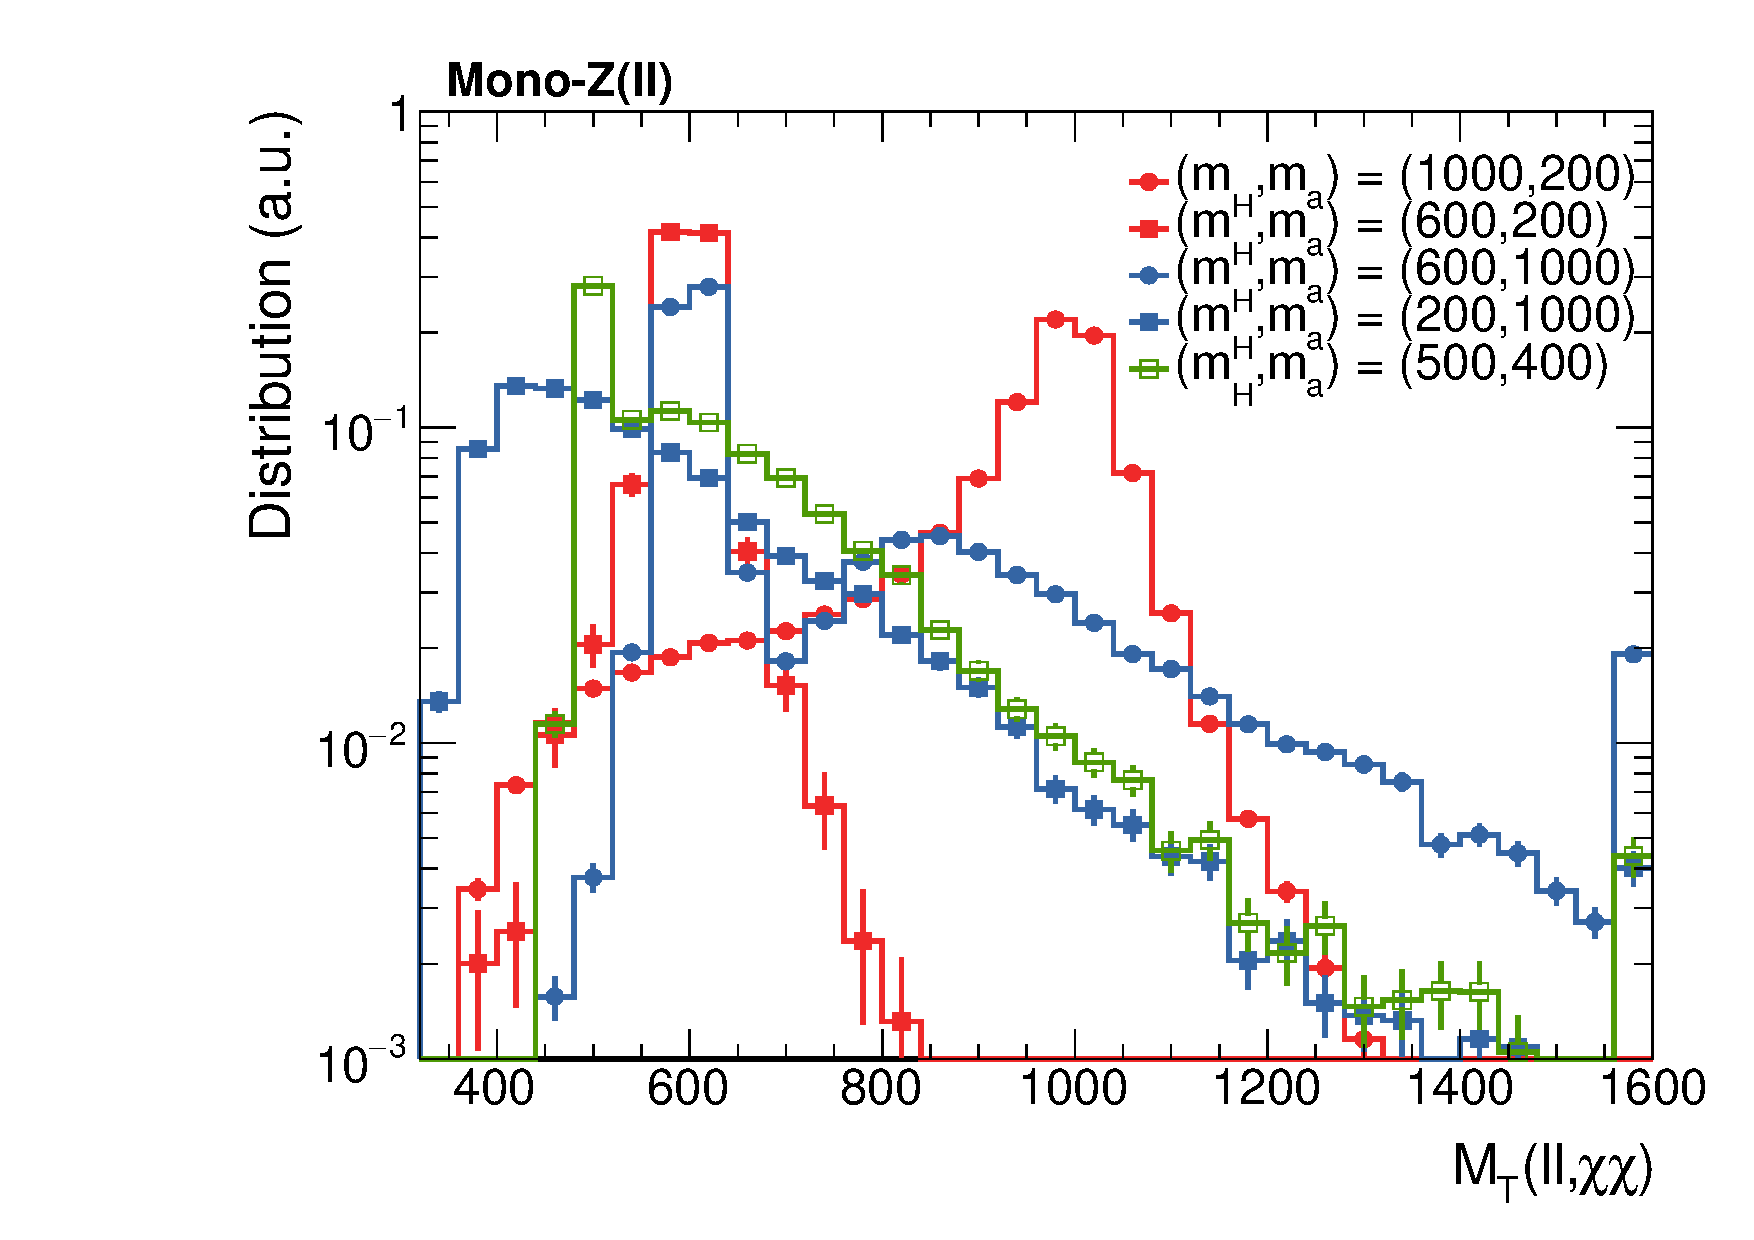
\includegraphics[width=0.45\textwidth]{texinputs/04_grid/figures/monoz/leptonic/dmwg-final_h_mt_total.pdf}
\caption{\MET and  $\MT$ distributions after the full selection of Z(lep)+\MET search. Both distributions show a peaked structure around $\mH$ in the $\mH > \ma$ regime, reflecting the resonant production of $H$ with a subsequent decay $\pH\to\pa\pZ$.\label{fig:monoz_kin_final}}

\end{figure}

In designing a search for evidence of this particular model, it may be useful to consider not only the $\MET$, but also the transverse mass $\MT$\footnote{The massless definition is used here: $\MT = \sqrt{2 \met p_{\rm{T,Z}} \left(1-\cos\left(\Delta\phi\right)\right)}$} variable. 
The distributions of both variables after final selection are shown in ~\autoref{fig:monoz_kin_final} for the Z+\MET searches. 
Both distributions show Jacobian peak structures due to dominant effect of the diagram with resonant H exchange. 
In the case of $\ma<\mH$, the peak structure is more defined in the \MT distribution than in the \MET, thus helping to distinguish a possible signal from background. 
Where the resonant diagram does not contribute, i.e. for $\ma\approx\mH$ or $\ma>\mH$, the \MT distribution does not show a significantly different structure from the \MET distribution and will not provide an improved sensitivity.

For mono-$h$, the \textbf{mass of the heavy neutral scalar Higgs boson} $\boldsymbol{H}$ has an indirect effect on the rate and kinematics of the signal. 
This is caused by the dependence of the coupling strength of the $a-A-h$ vertex, and thus decay width of the pseudoscalar $A$, on  $\mH$~\cite{Bauer:2017ota}. 
Therefore, a change of $\mH$ can strongly affect the relative contribution of resonant versus non-resonant signal processes, as illustrated in \autoref{fig:monoHbb_mH_scan_met}.
For mono-$Z$, there is no corrresponding effect of $\mA$ on the resonant and non-resonant signal yields, since the $a-H-h$ vertex has a simpler structure with no $\mA$ dependence.

The choice $\mH = \mA$ results in a detectable total cross section and a dominant contribution of the resonant mono-$h$ signal process for many signal points. 
%Do we show this somewhere?
This choice allows us to test diverse $\MET$ distributions and results in about equal contributions to the sensitivity through the \monoz and \monoh signatures, highlighting their complementarity. 
For this reason \emph{the choice $\mH = \mA$ is adopted} for all scans.  

The mass of the neutral scalar $H^{\pm}$ does not affect the model kinematics, as shown in Appendix~\autoref{KinematicPlotsAppendix}.
Models with $\mHc\neq\mH$ are moreover strongly constrained by electroweak precision measurements of the $\rho$ parameter~\cite{Bauer:2017ota}.
Therefore, for simplicity, the \emph{neutral scalar $H^{\pm}$ is assumed to be mass-degenerate to $H$}.

%as demonstrated in \autoref{fig:monoHbb_mA_scan_met} and \autoref{fig:monoHbb_ma_scan_met}

\begin{figure}[!htbp]
	\centering

%	\begin{subfigure}[t]{0.7\textwidth}
%	\centering
	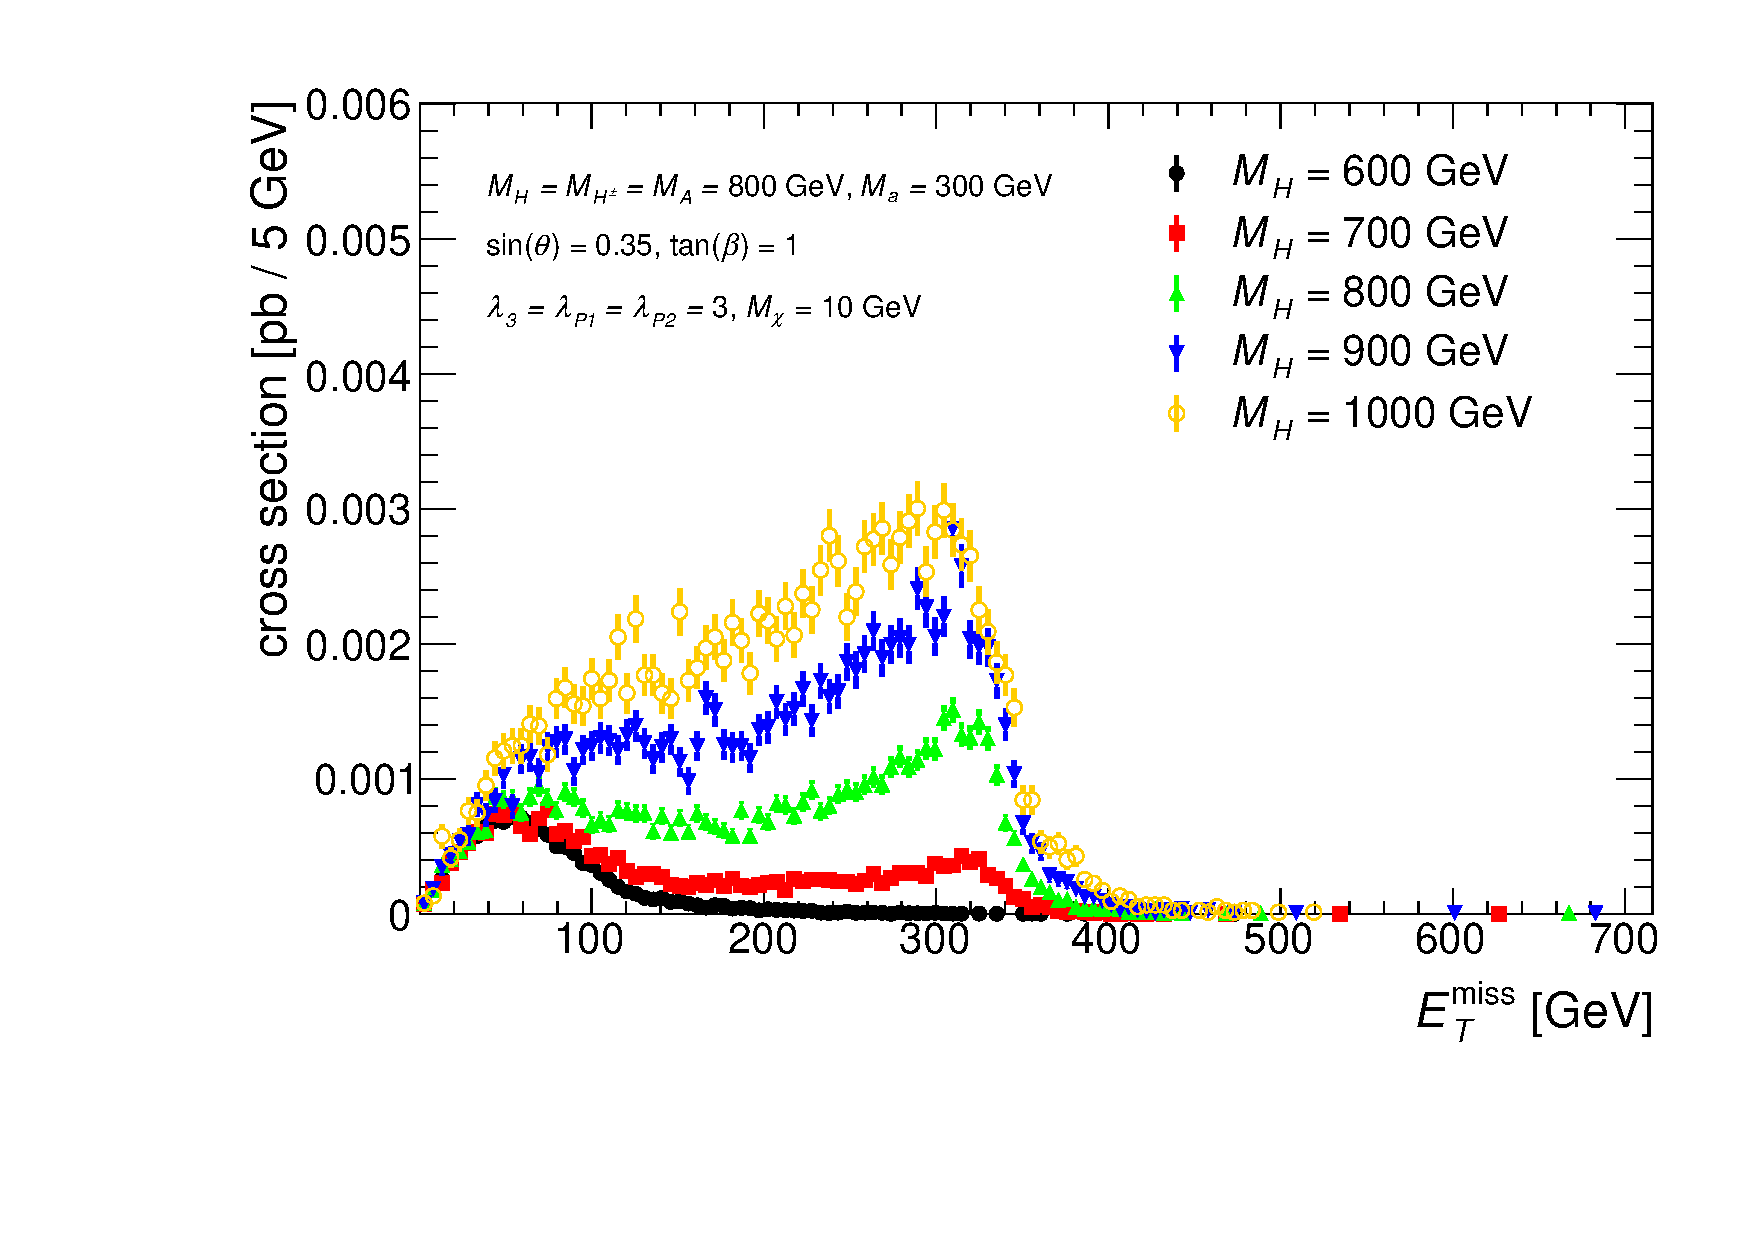
\includegraphics[width=0.7\textwidth]{texinputs/04_grid/figures/monoHbb_mH_scan_MET_liny.pdf}
	\caption{The \MET distribution, accounting for the production cross section, of \monohbb signal events for five representative choices of $\mH = \mHc$.
	%and fixed $ \mA=800$ GeV, $\ma = 300 $ GeV,  $ \sinp = 0.35, \tanb = 1, \mDM = 10$ GeV and $ \lap1 = \lap2 = \lam3 = 3 $.
	\label{fig:monoHbb_mH_scan_met}} 
%    \end{subfigure}
     
	\caption{$\MET$ distribution in \monohbb and Z+\MET events for different $\mH$}
\end{figure}

\subsubsection[Mixing angle between the two pseudoscalars $A$ and $a$ ($\sinp$)]{Mixing angle between the two pseudoscalars $\boldsymbol{A}$ and $\boldsymbol{a}$ ($\boldsymbol{\sinp}$)}

The sine of the mixing angle between the two pseudoscalars $A$ and $a$, $\sinp$, affects not only the cross section, but also the shape of the \MET\ distribution in searches including a Higgs boson, as shown in \autoref{fig:monoHbb_sinp_scan_mA600_ma200_met}. 
For the resonant diagram $gg\rightarrow A \rightarrow ah \rightarrow \chi\bar{\chi}h$, the product of cross section times branching ratios ${\cal B}(A\rightarrow ah){\cal B}(a \rightarrow \chi\bar{\chi})$ scales with $\sin^2\theta\cos^6\theta$, while for the diagram $gg\rightarrow a \rightarrow A^*h \rightarrow \chi\bar{\chi}h$, the product of cross section times branching ratios ${\cal B}(a\rightarrow Ah){\cal B}(A \rightarrow \chi\bar{\chi})$ scales with $\sin^6\theta\cos^2\theta$. 
This is shown in Appendix~\autoref{KinematicPlotsAppendix}.
Therefore, at small \sinp, the resonant diagram $A\rightarrow ah$ is the dominant production mode and the \MET\ distribution has a Jacobian peak following \autoref{eq:monoH_peak_met}; while at large \sinp, the $a\rightarrow A^*h$ diagram starts to dominate and produces a second peak at a lower \MET\ value. 

\begin{figure}
  \centering
  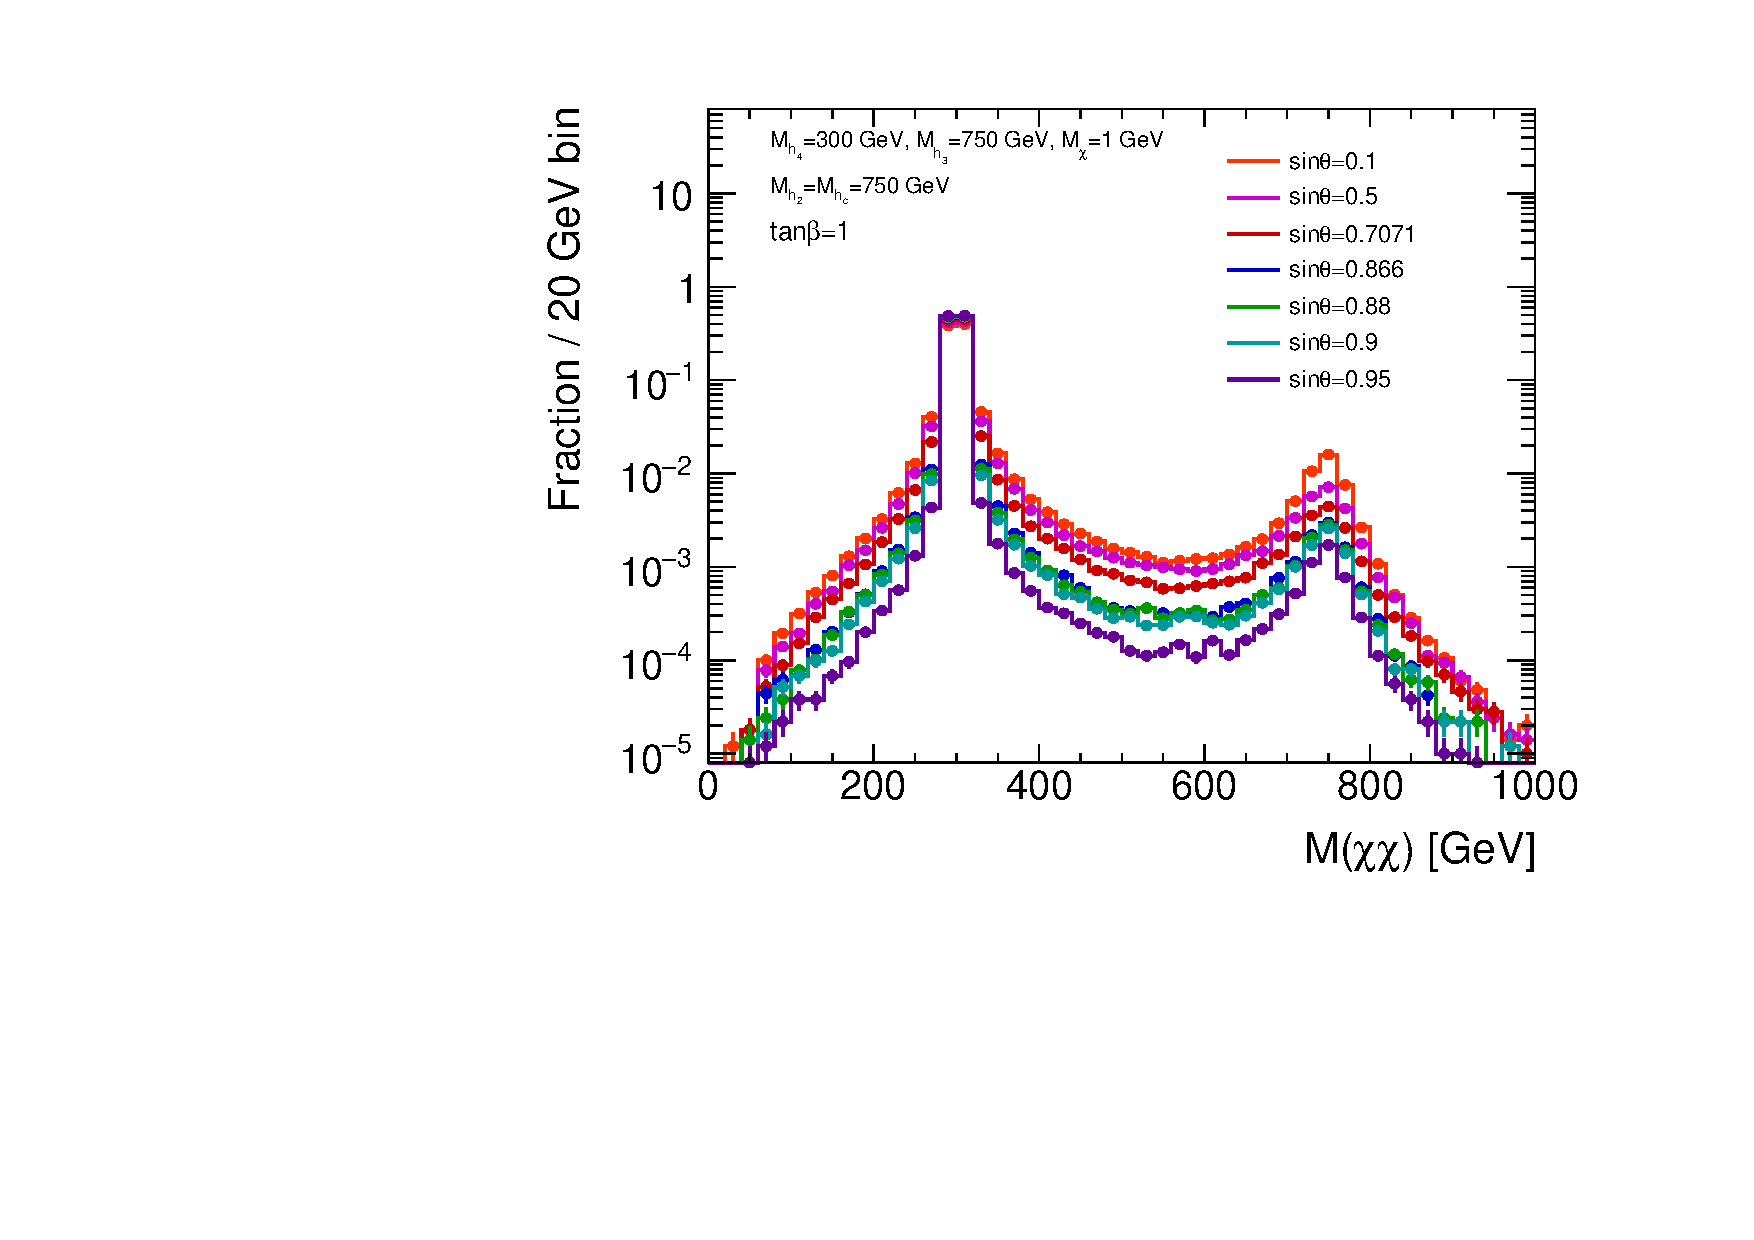
\includegraphics[width=0.6\textwidth]{texinputs/04_grid/figures/DMHF/benchmarking/MDM_1_Ma_300_MA_750_tanb_1.0_SCAN_sinp_v2/mchichi.pdf}
  \caption{The mass distribution of the $\chi \bar{\chi}$ system for various values of $\sin\theta$, with $\mathrm{M_a}=300$ GeV, $\mathrm{M_A}=750$ GeV, $\mathrm{M_H}=\mathrm{M_{H^{\pm}}}=750$ GeV, and $\tan\beta=1$.}
  \label{fig:mchichi_sinp}
\end{figure} 

\begin{figure}
  \centering
  \begin{subfigure}[b]{0.49\textwidth}
    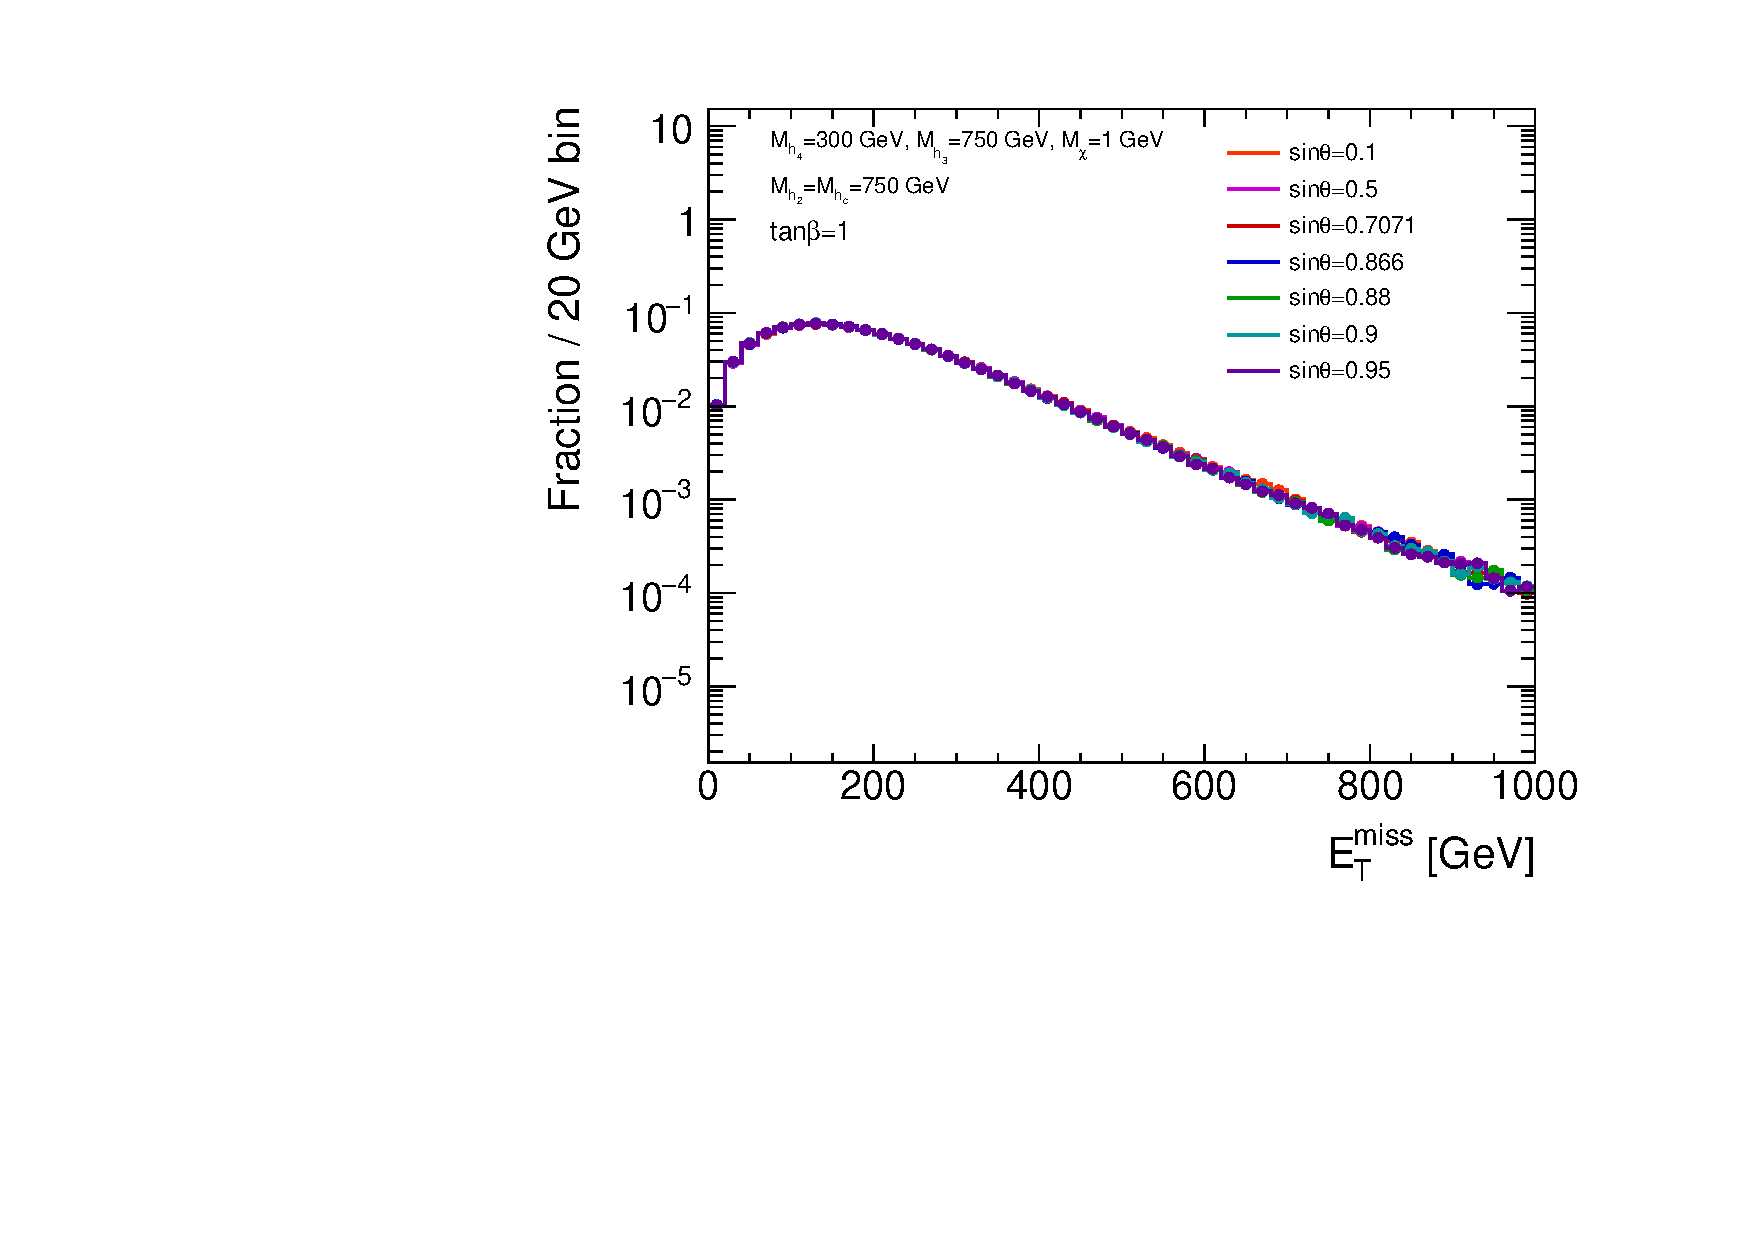
\includegraphics[width=\textwidth]{texinputs/04_grid/figures/DMHF/benchmarking/MDM_1_Ma_300_MA_750_tanb_1.0_SCAN_sinp_v2/metlog.pdf}
    \caption{$E_{T}^{miss}$}
  \end{subfigure}
  \begin{subfigure}[b]{0.49\textwidth}
    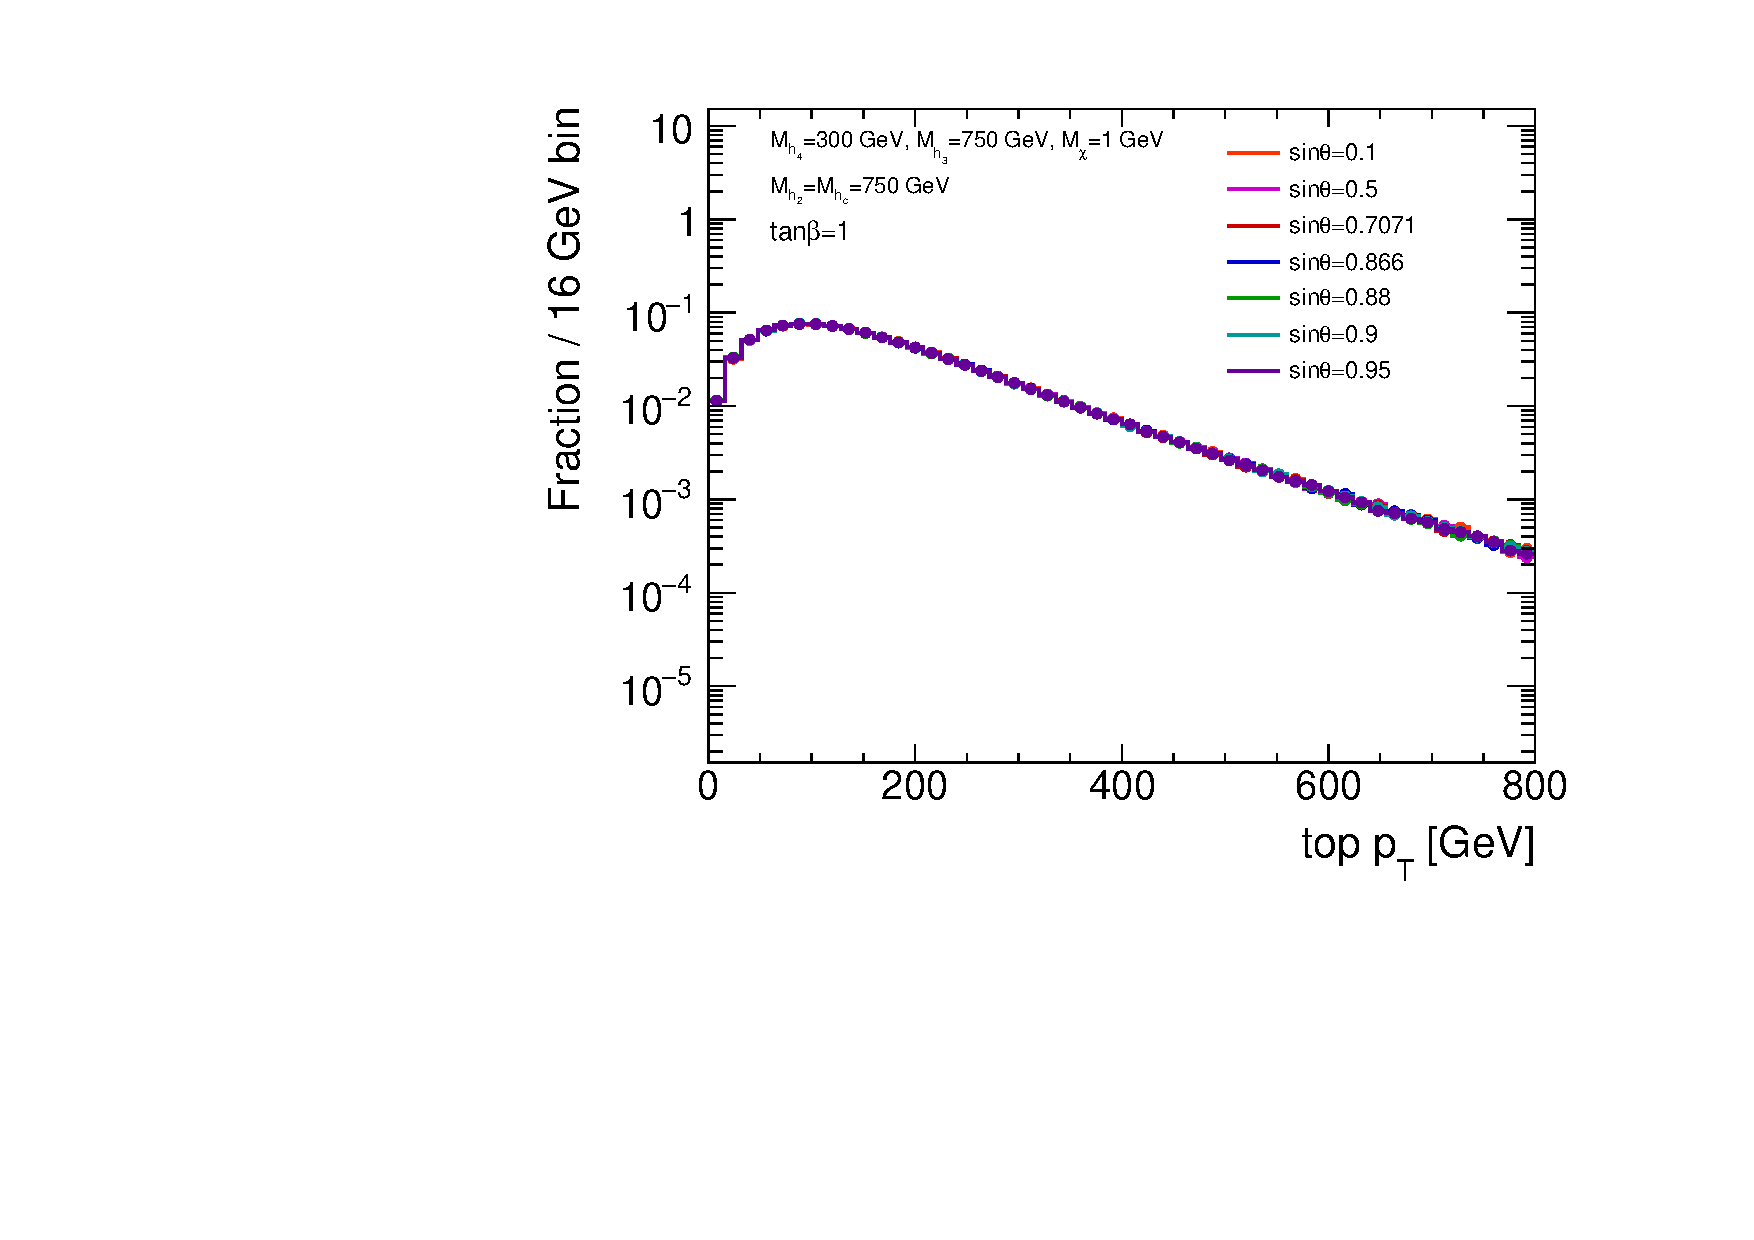
\includegraphics[width=\textwidth]{texinputs/04_grid/figures/DMHF/benchmarking/MDM_1_Ma_300_MA_750_tanb_1.0_SCAN_sinp_v2/topptlog.pdf}
    \caption{top $p_{T}$}
  \end{subfigure}
  \caption{The $E_{T}^{miss}$ and top $p_{T}$ distribution for inclusive $t\bar{t}+\chi\bar{\chi}$ production for various values of $\sin\theta$, with $\mathrm{M_a}=300$ GeV, $\mathrm{M_A}=750$ GeV, $\mathrm{M_H}=\mathrm{M_{H^{\pm}}}=750$ GeV, and $\tan\beta=1$.}
  \label{fig:kin_sinp}
\end{figure}

\begin{figure}%[!htbp]
	\centering

	\begin{subfigure}[t]{0.45\textwidth}
	\centering
	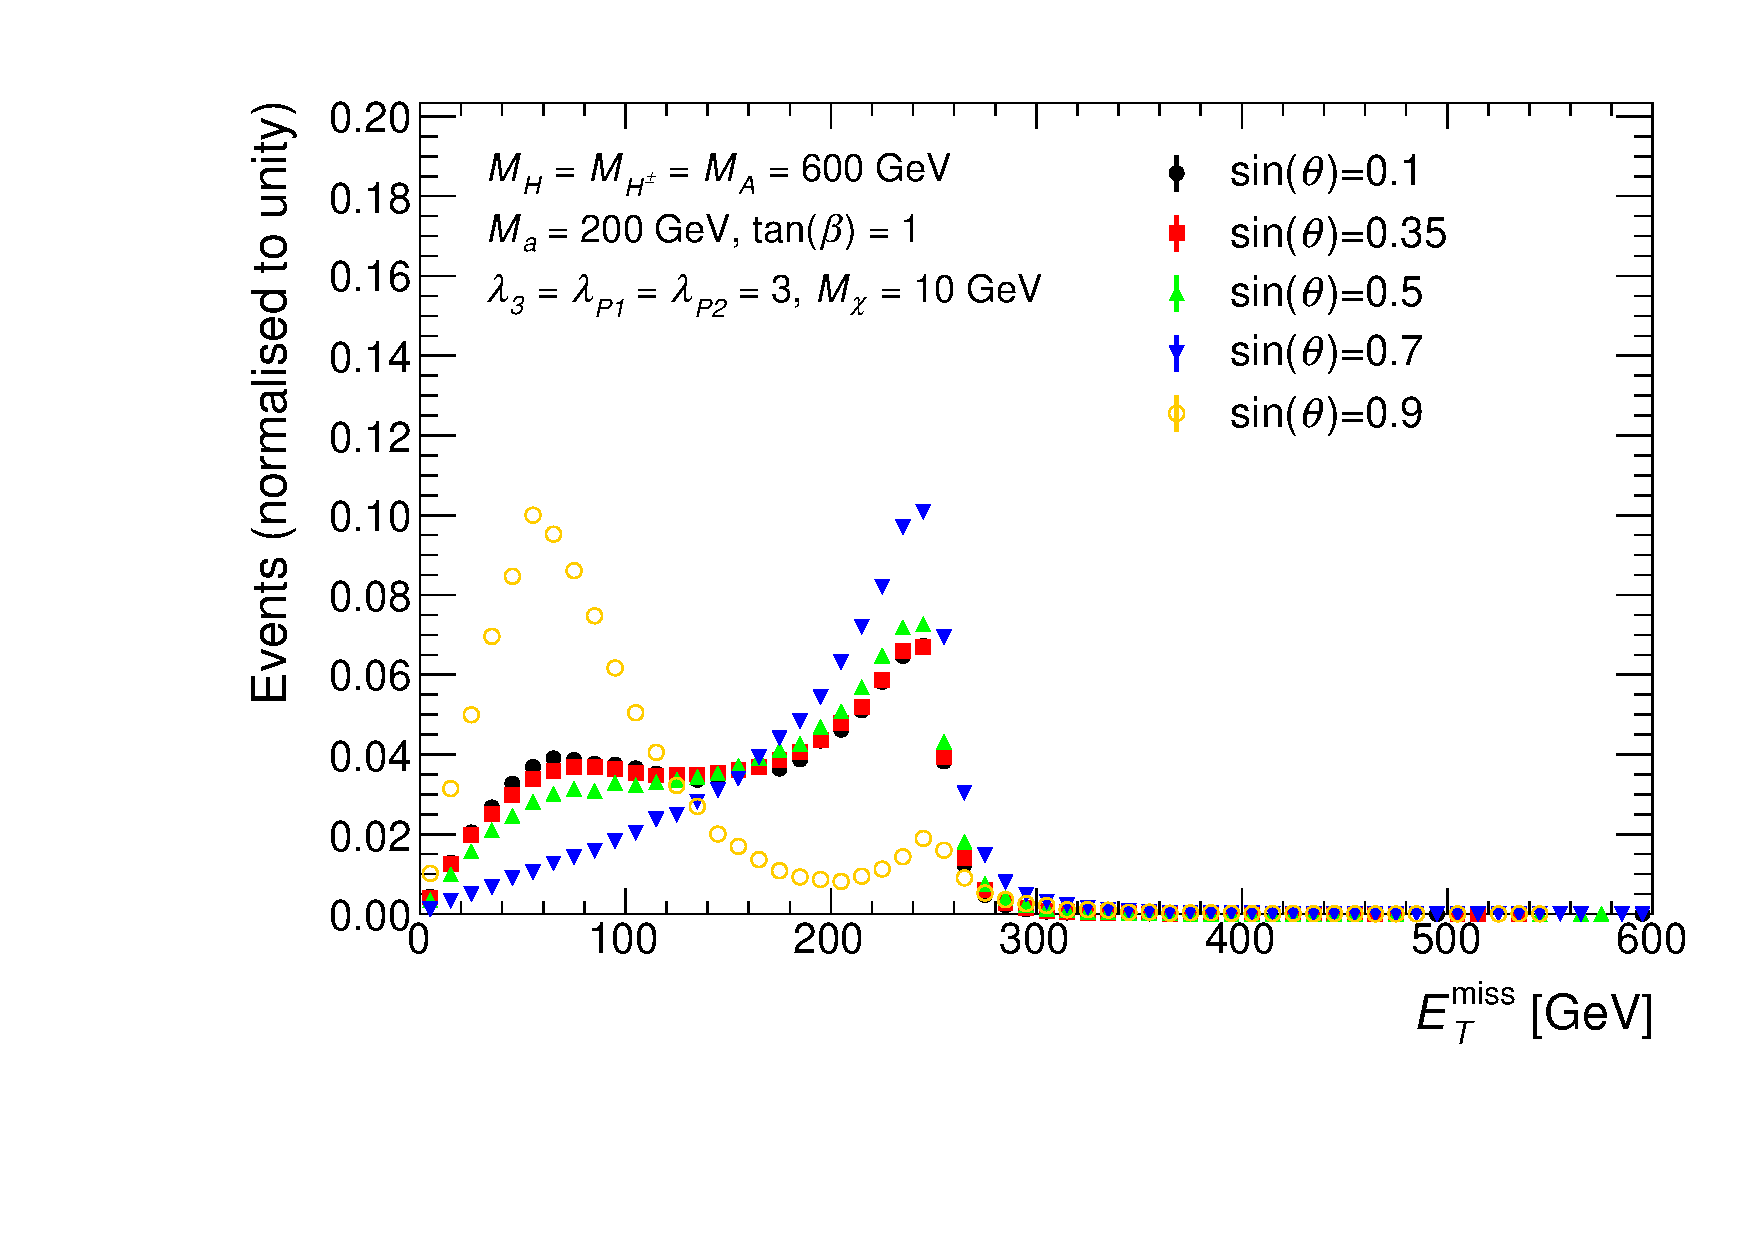
\includegraphics[width=\textwidth]{texinputs/04_grid/figures/monoHbb_sinp_scan_MA600_Ma200_MET_liny_norm2one.pdf}
	\caption{$\MET$ distribution for for five representative models with different $\sinp$ and fixed $\mA = \mH = \mHc = 600 $~GeV, $\ma = 200$~GeV.
	\label{fig:monoHbb_sinp_scan_mA600_ma200_met}} 
    \end{subfigure}
    \begin{subfigure}[t]{0.45\textwidth}
	\centering
	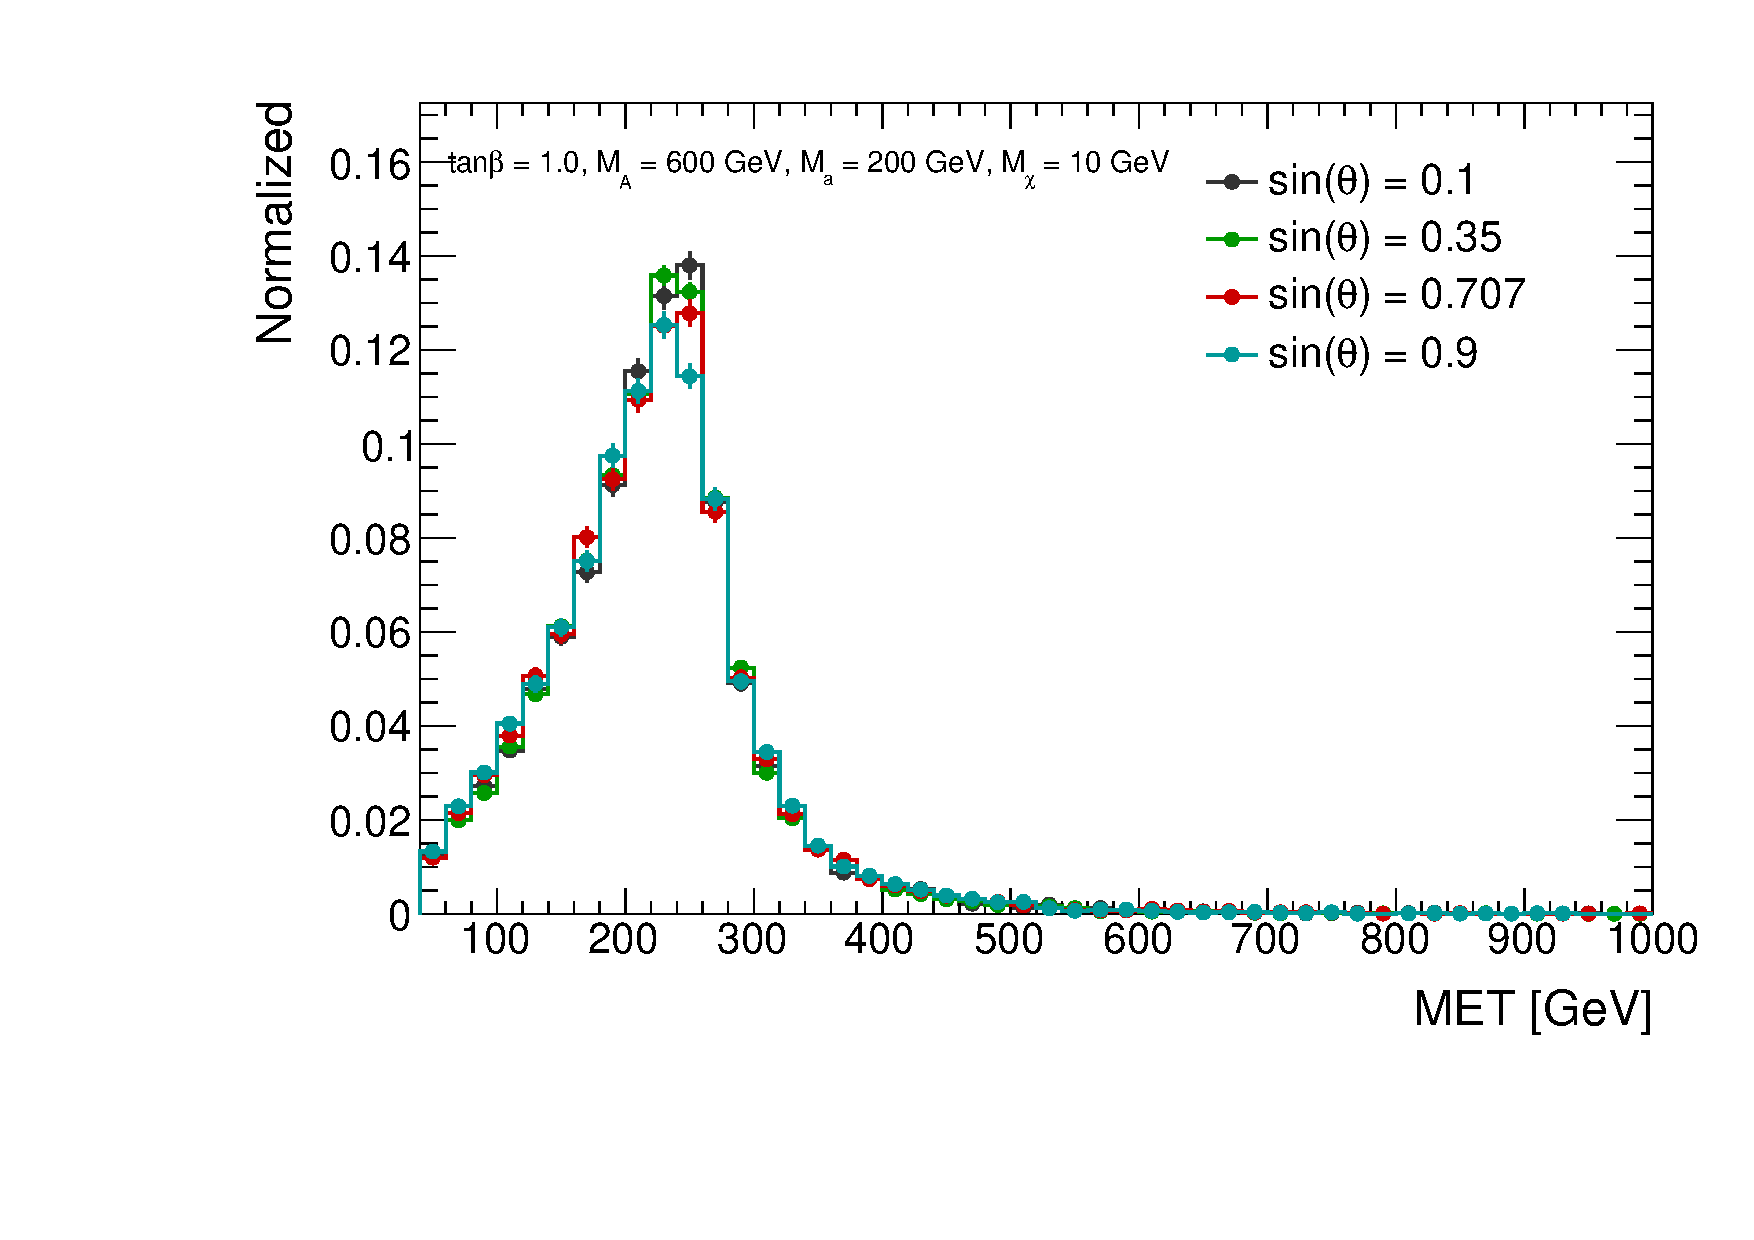
\includegraphics[width=\textwidth]{texinputs/04_grid/figures/monoz/leptonic/SinpScan_mA600_ma200_MET.pdf}	
	\caption{\MET distribution after preselection for scans of $\sin{\theta}$ for fixed $\mA = \mH = \mHc = 600 $~GeV and $\ma = 200 $~GeV.
	\label{fig:monoz_kin_sintheta}}
    \end{subfigure}
    
    \caption{$\MET$ distributions in \monohbb and Z(lep)+\MET events for different $\sin{\theta}$. In both cases, $\tanb = 1$ and $\mDM = 10$~GeV. }
    
\end{figure}

%In the \monohbb case, the shape of the $\MET$ distribution does not change much  for $\sinp < 0.7$, then changes significantly for $\sinp\geq 0.7$. 
%When $\sinp=0.9$, the diagram $gg\rightarrow a\rightarrow A^*h \rightarrow \chi \bar{\chi} h$, producing a \MET peak at around 60~GeV, starts to dominate.
%Lars: The above is true _only_ for this particular mass configuration. Either we leave this out, or we write something about the mass-hierarchy dependence of the sintheta effect on mono-h.
%      In that case I would suggest showing the second scan with m_a > 2 * m_top to demonstrate this.

%Following these studies, \emph{it is desirable to scan $\sinp$ separately in the resonant and non-resonant regime}. 
%Lars: This is not the motivation for scaning sintheta at the two different mass points. The scan explores how sintheta, mH lambda3 etc. affect the monoHbb kinematics, and
%      there are two scans because for sintheta, this depends on the mass hierarchy of a, A w.r.t. DM, top.

Scans of the \sinp parameter show they have minimal effect on the kinematic distributions for searches with a Z boson (\autoref{fig:monoz_kin_sintheta}). 

%Mixing of the CP-odd weak eigenstates is achieved through the mixing angle, $\theta$. 
In the $t\bar{t}$ + \MET signature, the $A$ ($h_{3}$ in the figure) and $a$  ($h_{4}$ in the figure) mass peaks are quite narrow for values where $\sin\theta$ approaches 1, and $a\rightarrow\chi\bar{\chi}$ is the dominant $\chi\bar{\chi}$ production mode, as shown in \autoref{fig:mchichi_sinp}. 
However, no significant kinematic dependence on $\sin\theta$ is observed in the $E_{T}^{miss}$ and top quark $p_{T}$ as shown in \autoref{fig:kin_sinp} before any analysis cuts are applied.

\subsubsection[Ratio of the doublet vacuum expectation values ($\tanb$)]{Ratio of the doublet vacuum expectation values ($\boldsymbol{\tanb}$)}

\begin{figure}[tbp]
\centering
\begin{subfigure}{0.48\textwidth}
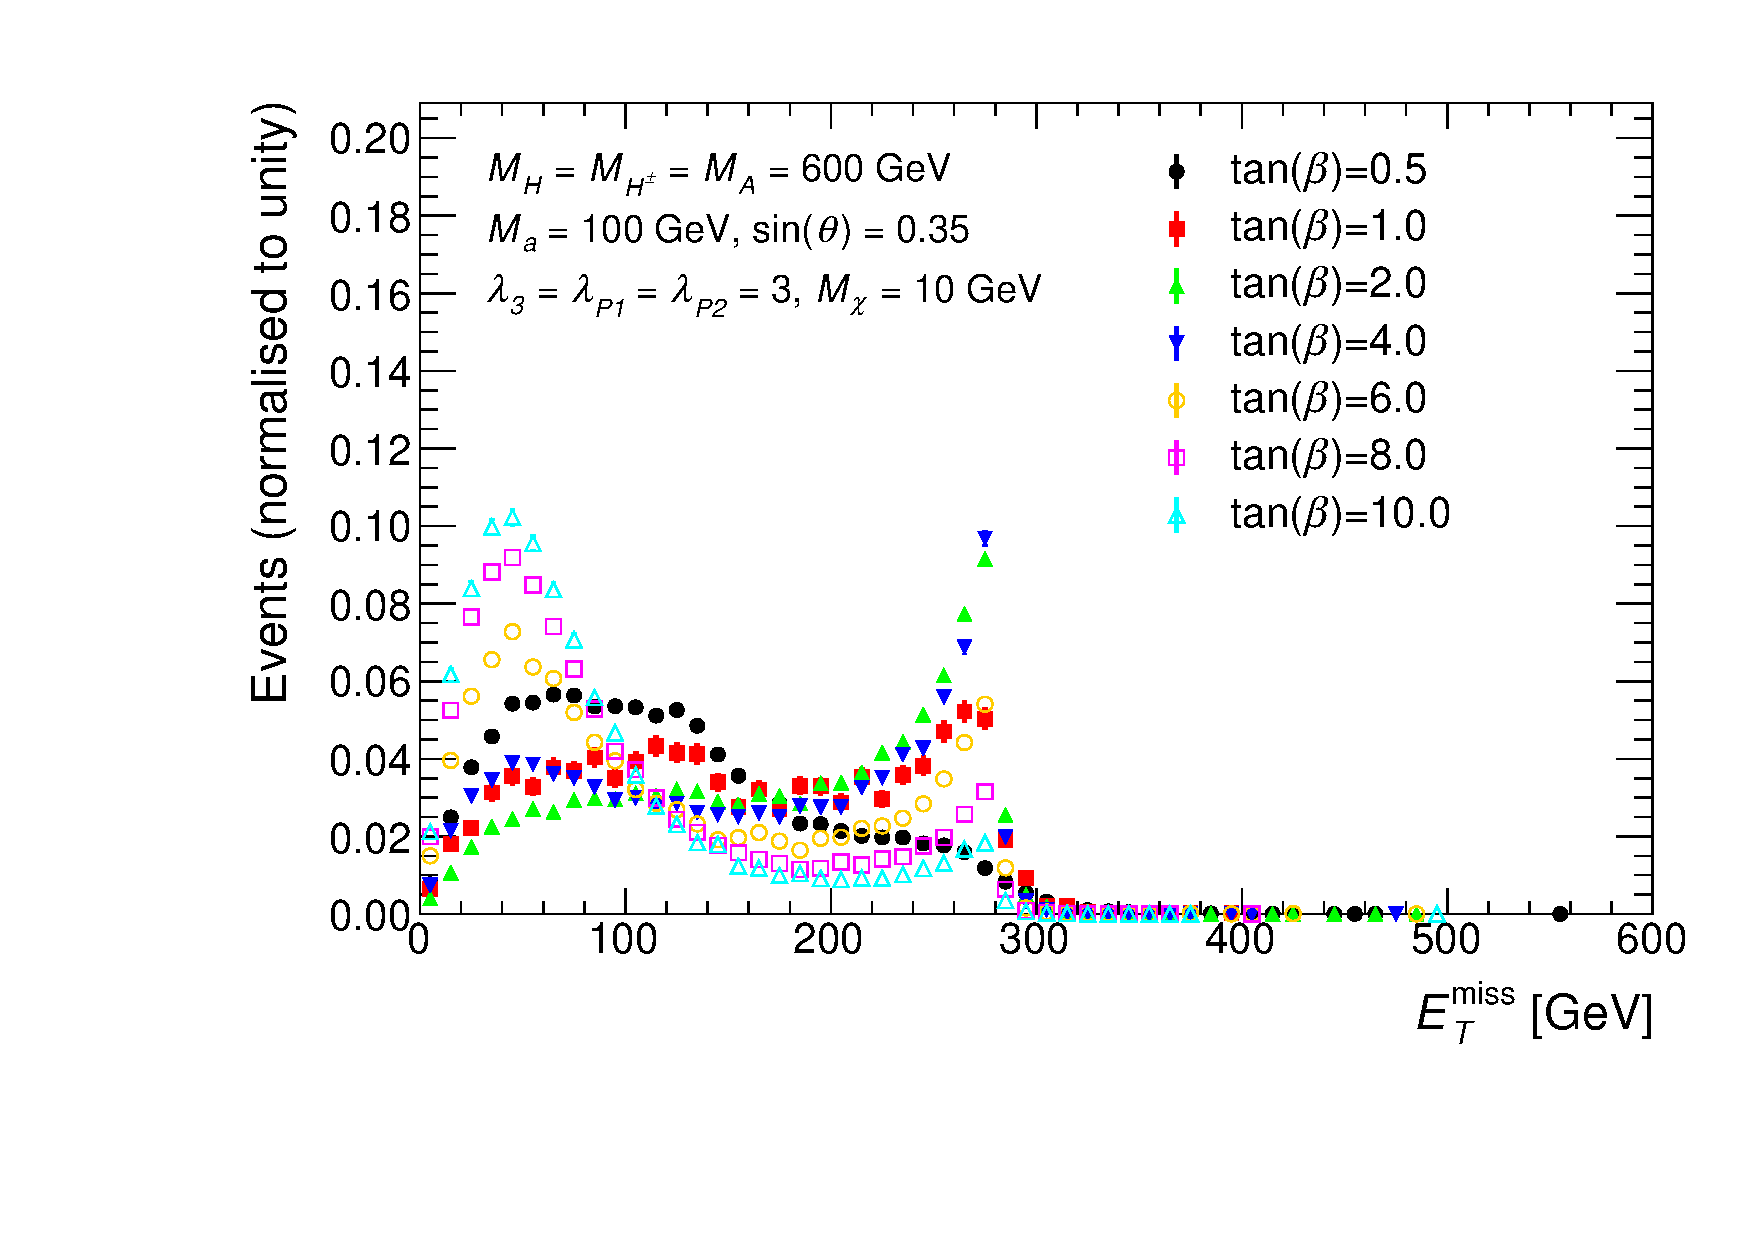
\includegraphics[width = \textwidth]{texinputs/04_grid/figures/monoHbb_tanb_scan_MA600_Ma100_MET_liny_norm2one.pdf}
\end{subfigure}
~
\begin{subfigure}{0.48\textwidth}
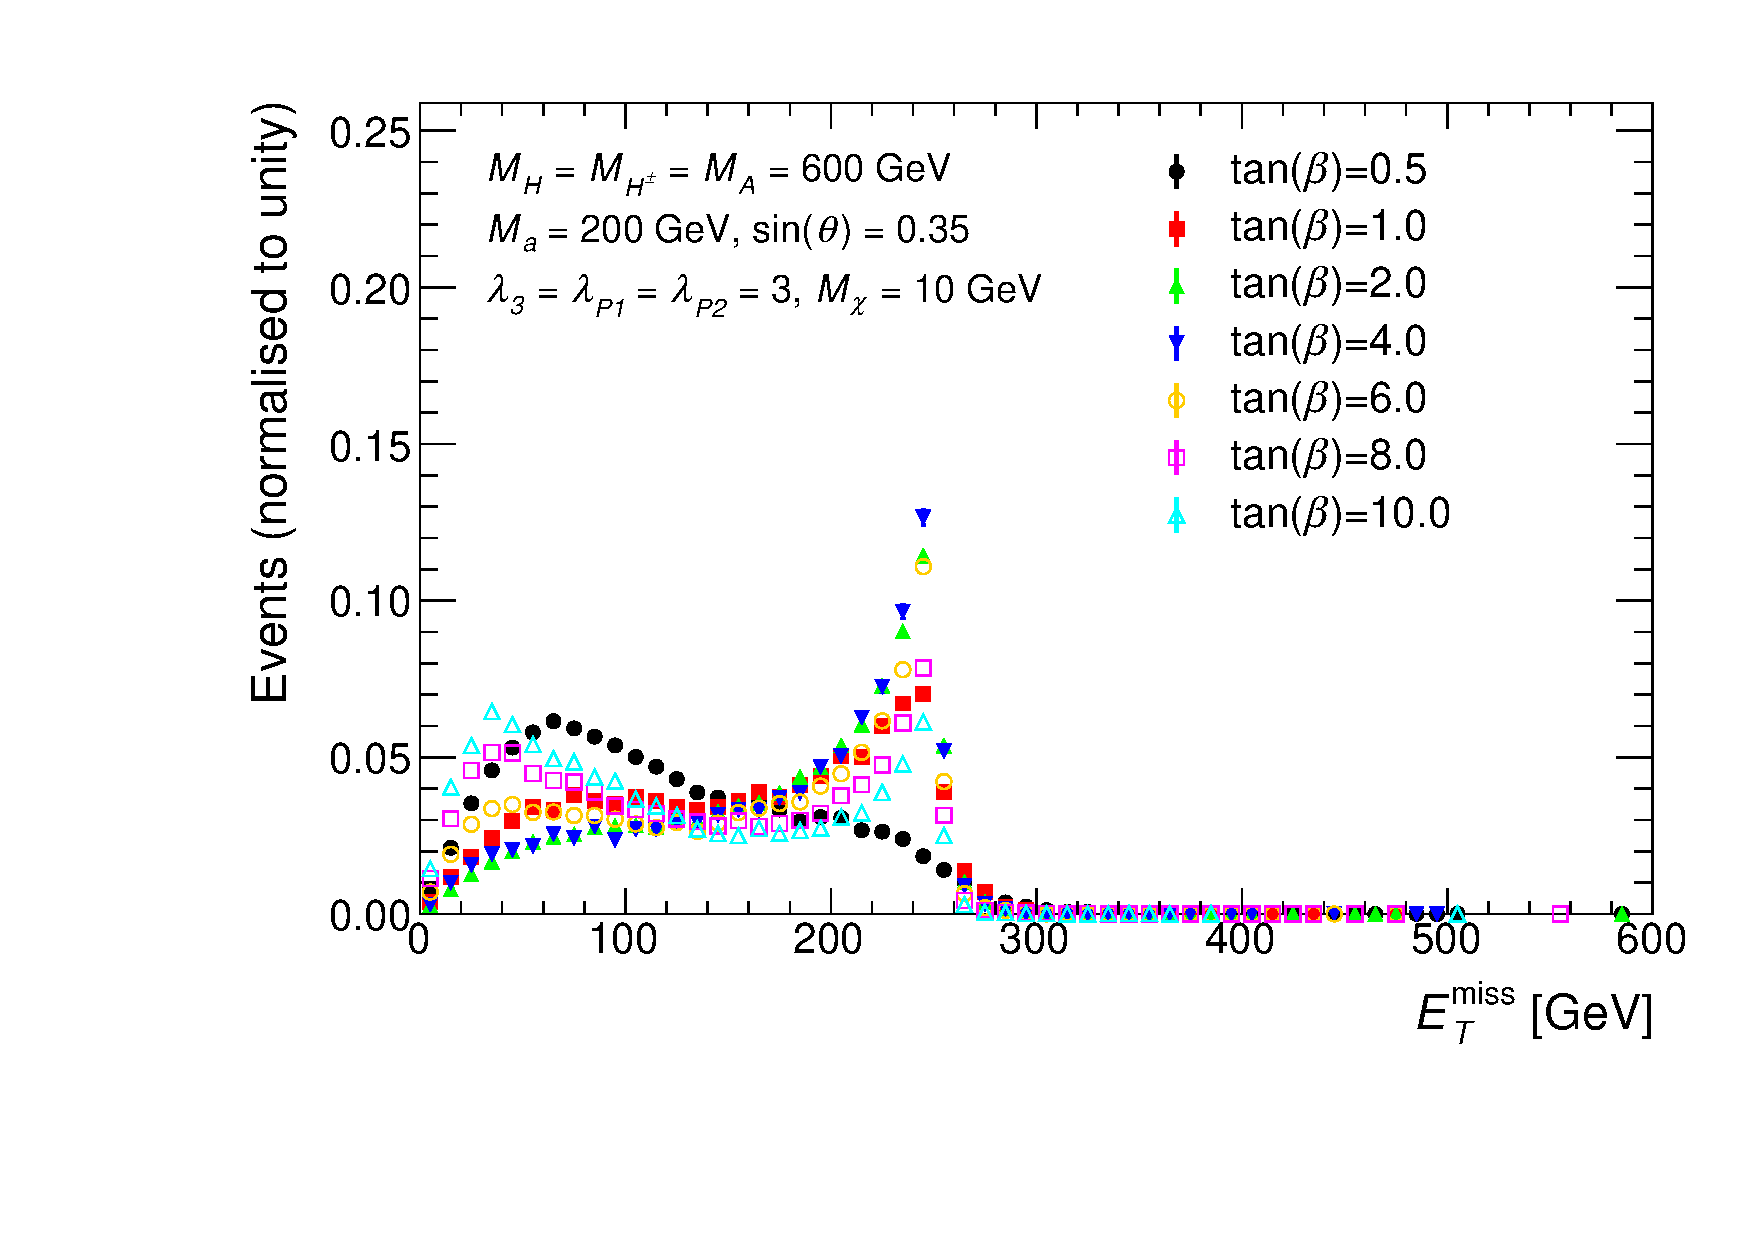
\includegraphics[width = \textwidth]{texinputs/04_grid/figures/monoHbb_tanb_scan_MA600_Ma200_MET_liny_norm2one.pdf}
\end{subfigure}
\\
\centering
\begin{subfigure}{0.48\textwidth}
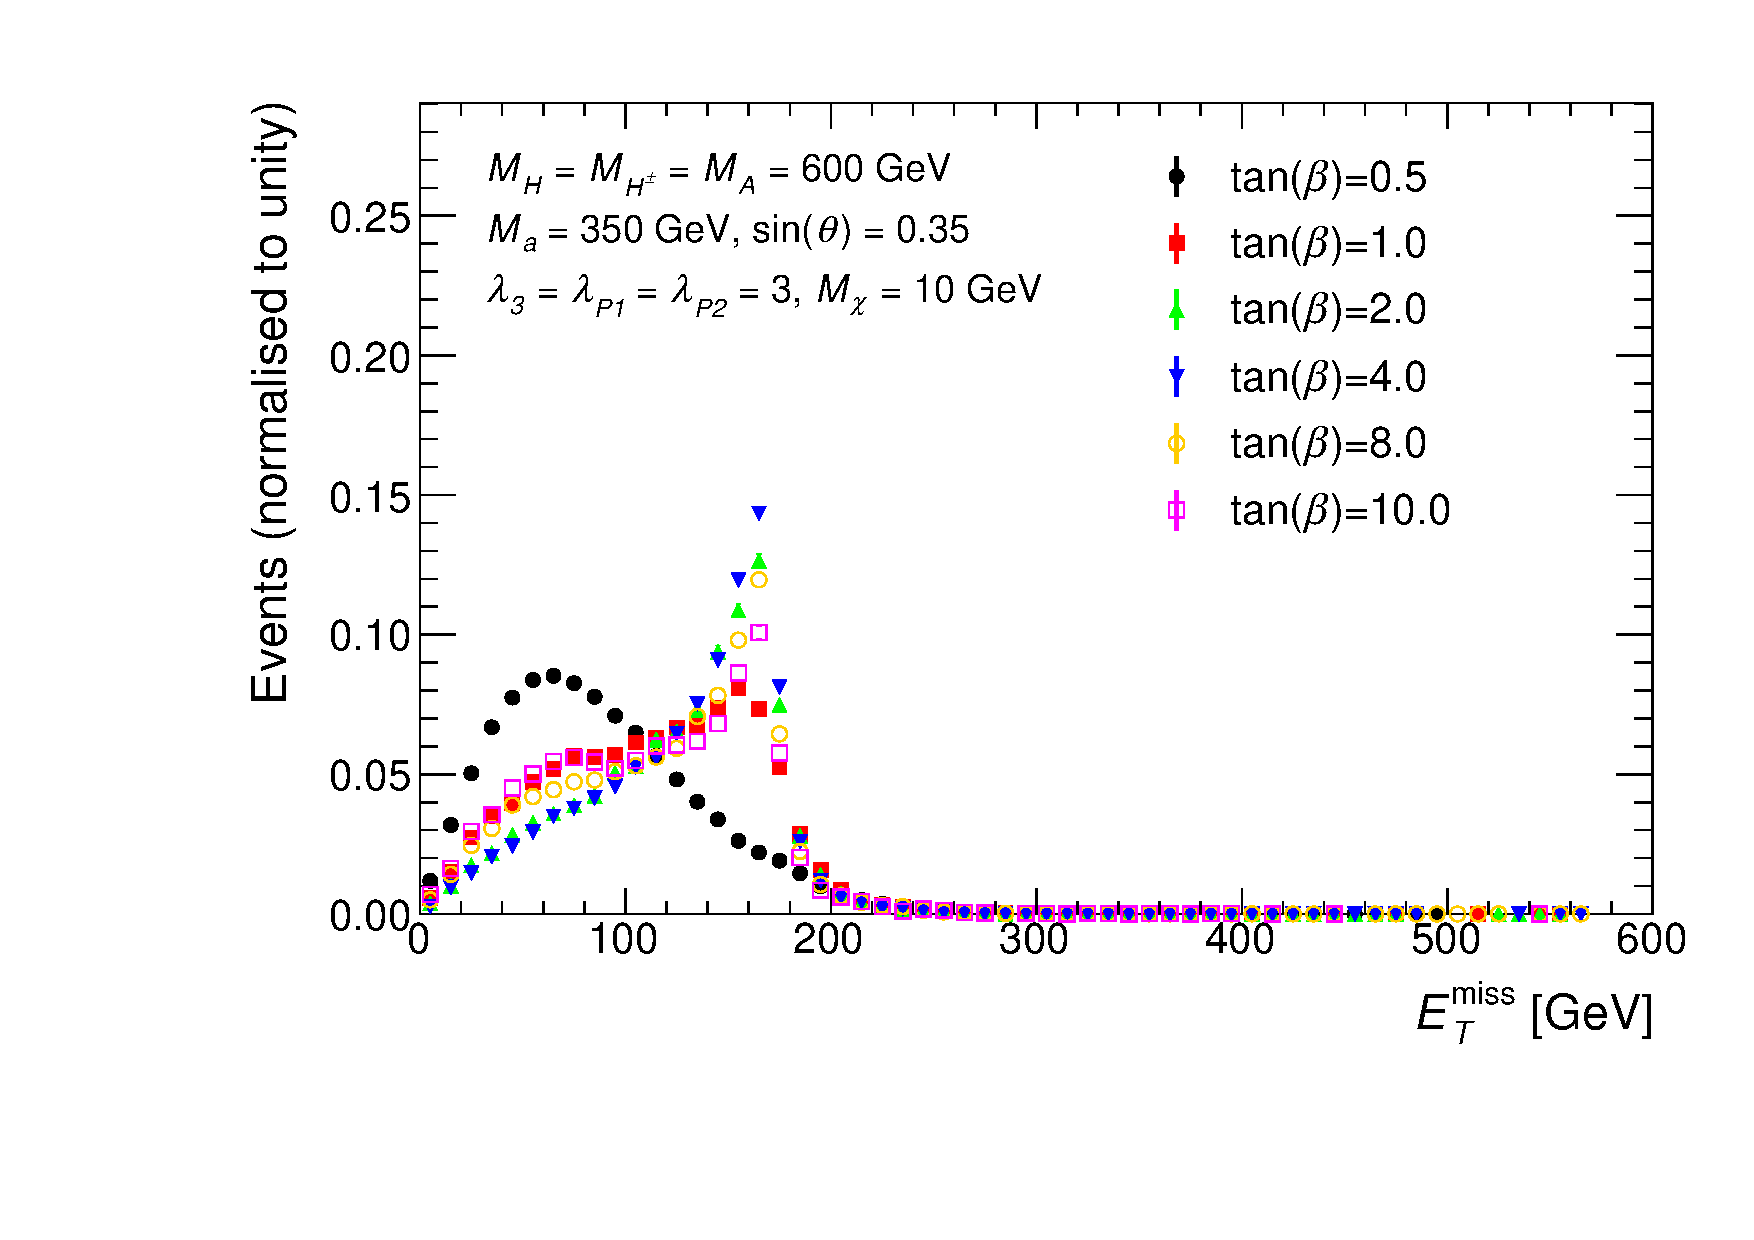
\includegraphics[width = \textwidth]{texinputs/04_grid/figures/monoHbb_tanb_scan_MA600_Ma350_MET_liny_norm2one.pdf}
\end{subfigure}
~
\begin{subfigure}{0.48\textwidth}
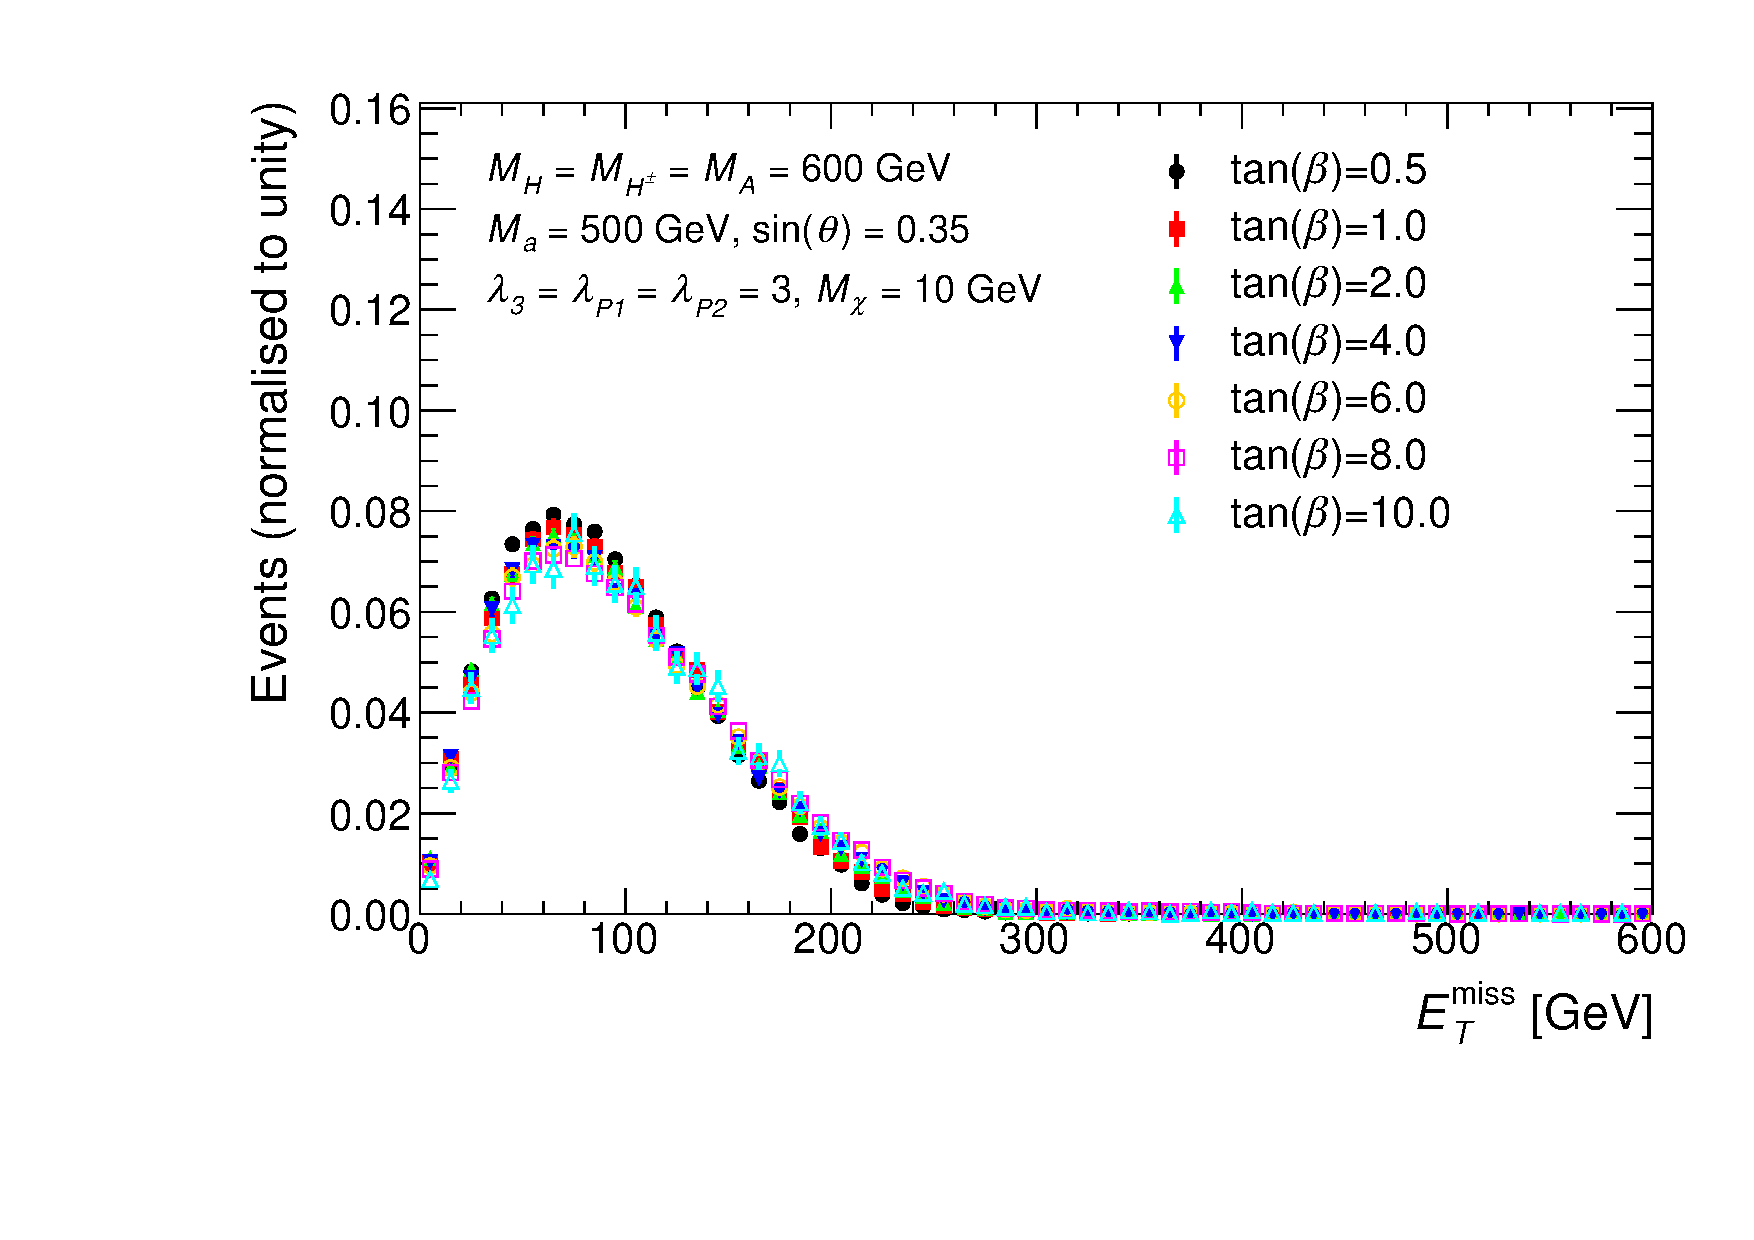
\includegraphics[width = \textwidth]{texinputs/04_grid/figures/monoHbb_tanb_scan_MA600_Ma500_MET_liny_norm2one.pdf}
\end{subfigure}
\caption[$\MET$ distribution in $h\rightarrow bb + \MET$ events for different 
$\tanb$ for $\mA = \mH = \mHc = 600 $ GeV]
{
Missing transverse momentum distribution of $h\rightarrow bb + \MET$ signal 
events at parton level with different $\tanb$ and
 fixed $\mA = \mH = \mHc = 600 $~GeV, $ \mDM = 10$~GeV, $\sinp = 0.35$, 
and $ \lap1 = \lap2 = \lam3 = 3 $. The values of $\ma$ are set to 100, 200, 
350, and 500~GeV, respectively.
The shapes of the $\MET$ distributions for different $\tanb$ are similar when 
$\mA < \mh+\ma$. Note, in these figures, both the contributions of $gg$ and $b\bar{b}$ 
initiated processes are included and a combined histogram is produced 
according to their corresponding cross sections.
\label{fig:monoHbb_tanb_scan_met}
}
\end{figure}

\begin{figure}
\centering
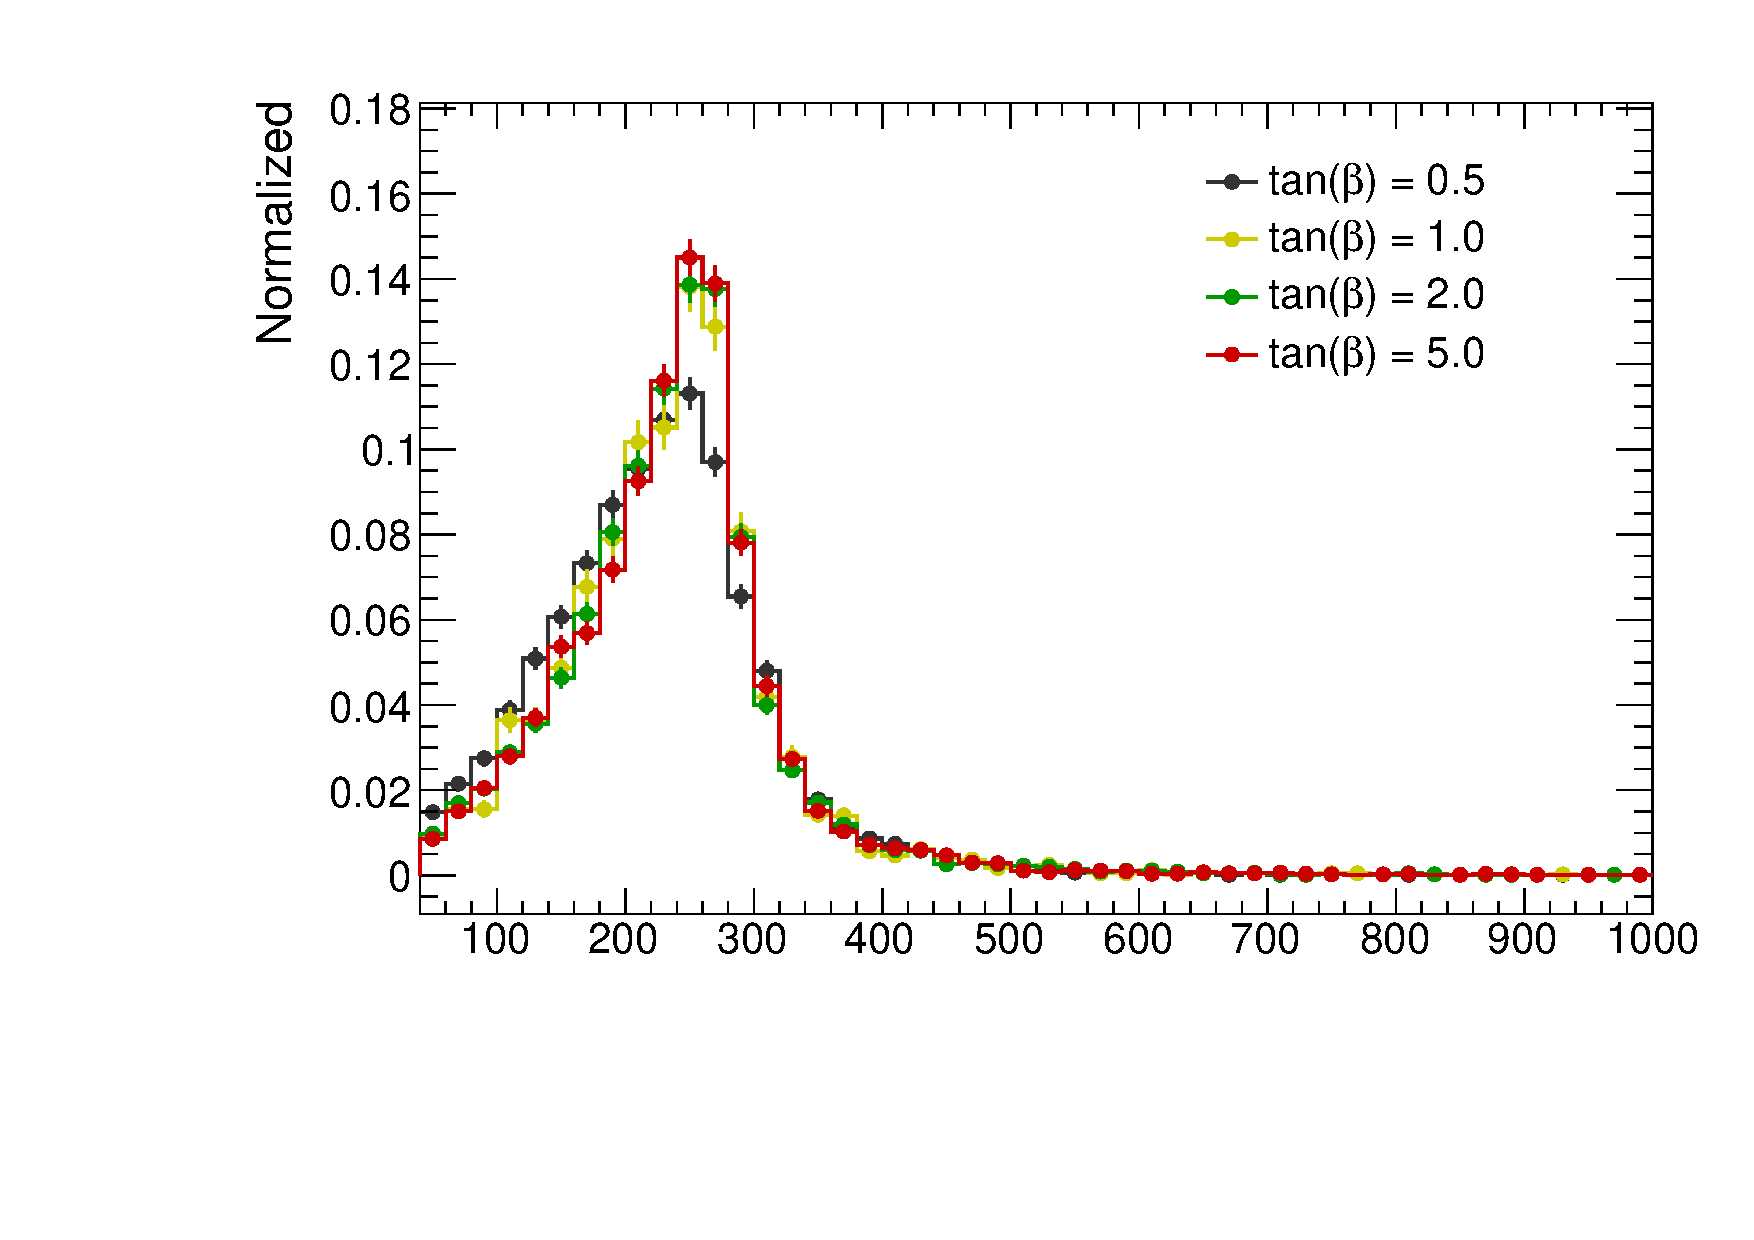
\includegraphics[width=0.7\textwidth]{texinputs/04_grid/figures/monoz/leptonic/TanbScan_mA600_ma150_MET.pdf} 
\caption{\MET distribution after preselection for scans of $\tan{\beta}$ for fixed \mA =600 \GeV and \ma = 150 \GeV. 
This parameter has little impact on the kinematic distributions, except for small values of \tanb where there is a slight softening and broadening of the \MET distribution caused by the increased contribution from the top box feynman diagram.}
\label{fig:monoz_kin_tanb}
\end{figure}

%%% text related to tanbeta-ma scan
The shape of \MET\ distribution also has a non-trivial dependence on \tanb, as can be seen in \autoref{fig:monoHbb_tanb_scan_met}.
As discussed in the sensitivity study later, at small \tanb, the Yukawa coupling to top quark is large and the signal production mode is dominated by the non-resonant 3-body processes $gg\rightarrow h\chi\bar{\chi}$, which gives a broad and soft \MET\ spectrum. 
As \tanb increases, the contribution of resonant production increases as well and the Jacobian peak also appears.
When the pseudoscalar $A$ is produced off-shell, i.e. when $\mA<\ma+\mh$, the shapes of \MET\ distributions become similar and the dependence on \tanb disappears.
For small values of $\tanb$ there is a slight softening and broadening of the \MET distribution caused by the increased contribution from non-resonant $Z+a$ production in Z+\MET searches. 

\begin{figure}
  \centering
  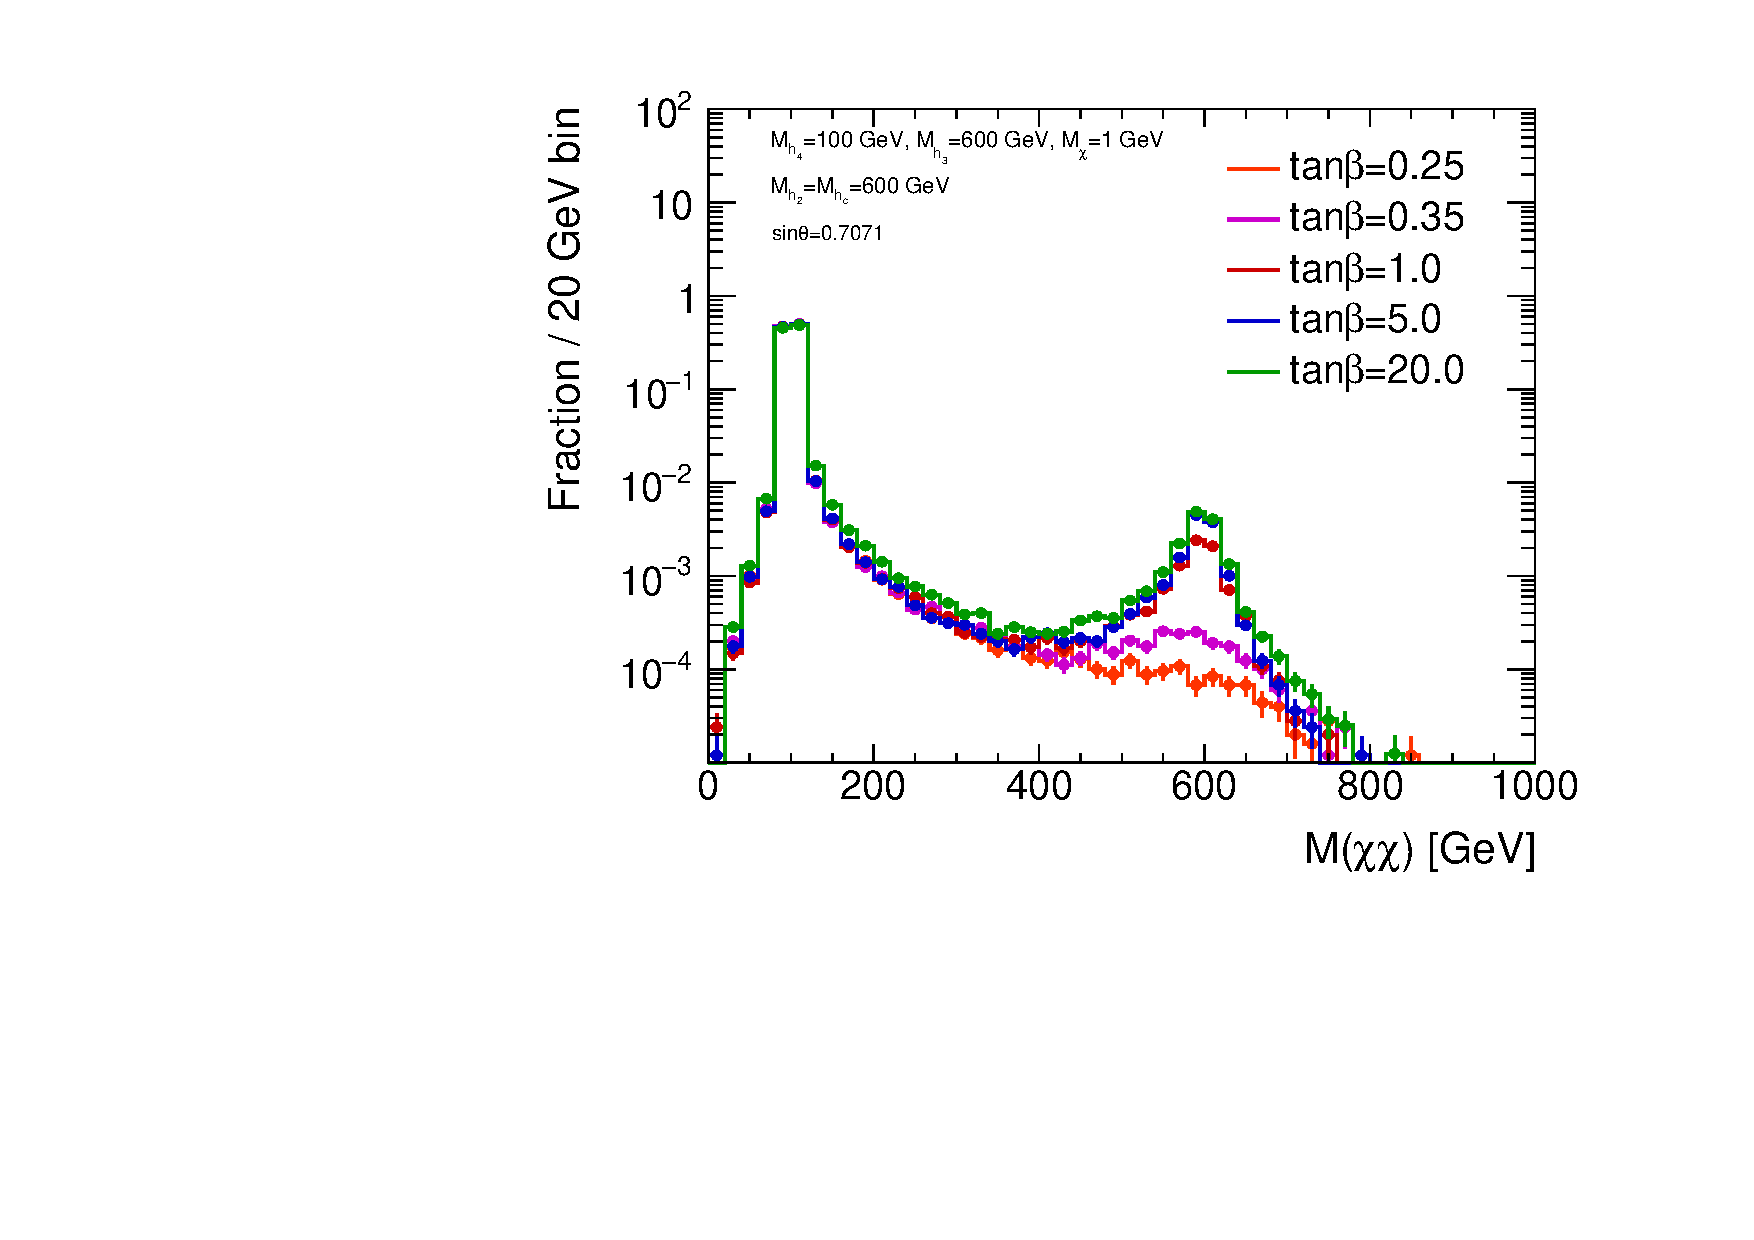
\includegraphics[width=0.7\textwidth]{texinputs/04_grid/figures/DMHF/benchmarking/MDM_1_Ma_100_MA_600_sinp_0.7071_SCAN_tanb_decayed/mchichi.pdf}
  \caption{The mass distribution of the $\chi \bar{\chi}$ system for various values of $\tan\beta$, with $\mathrm{M_a}=100$ GeV, $\mathrm{M_A}=600$ GeV, $\mathrm{M_H}=\mathrm{M_{H^{\pm}}}=600$ GeV, and $\sin\theta=0.7071$.}
  \label{fig:mchichi_tanB}
\end{figure}

\begin{figure}
  \centering
  \begin{subfigure}[b]{0.45\textwidth}
    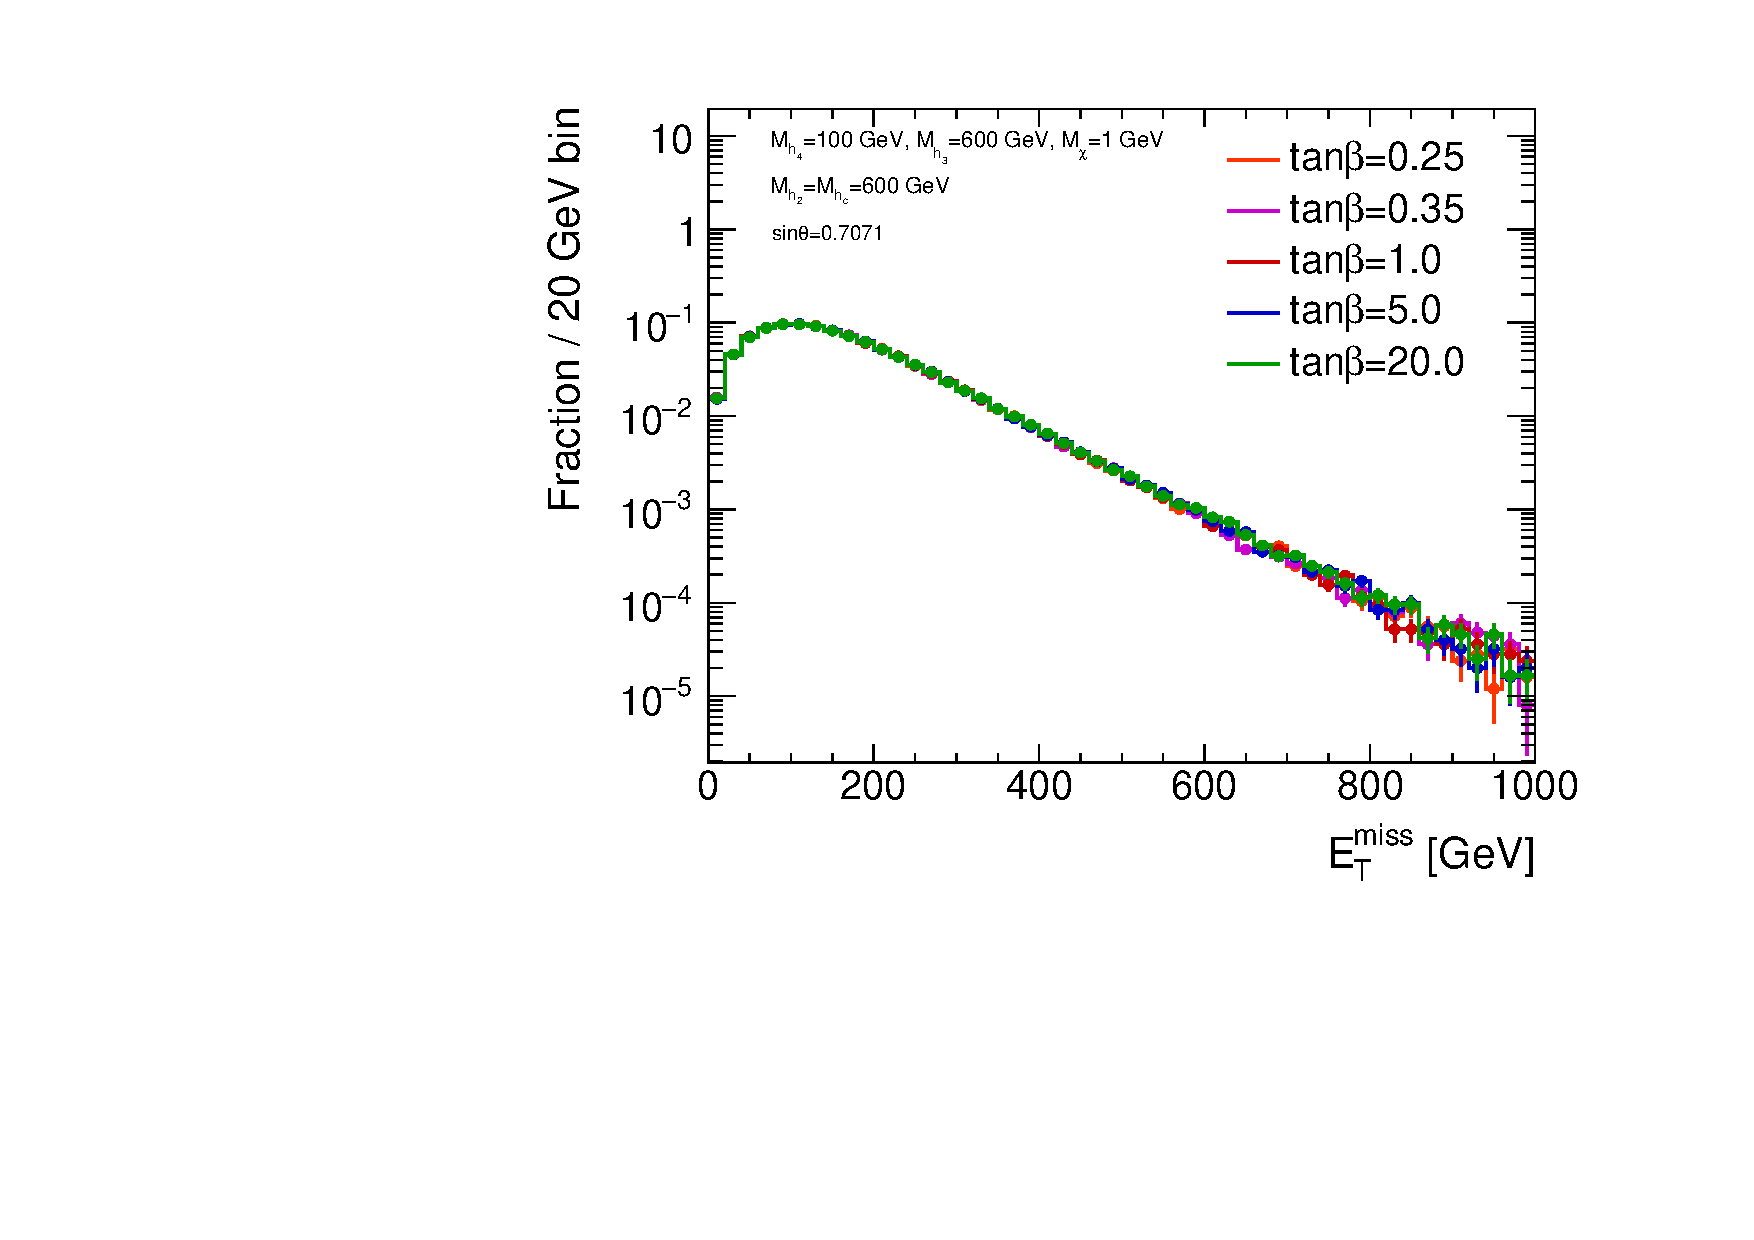
\includegraphics[width=\textwidth]{texinputs/04_grid/figures/DMHF/benchmarking/MDM_1_Ma_100_MA_600_sinp_0.7071_SCAN_tanb_decayed/metlog.pdf}
    \caption{$E_{T}^{miss}$}
  \end{subfigure}
  \begin{subfigure}[b]{0.45\textwidth}
    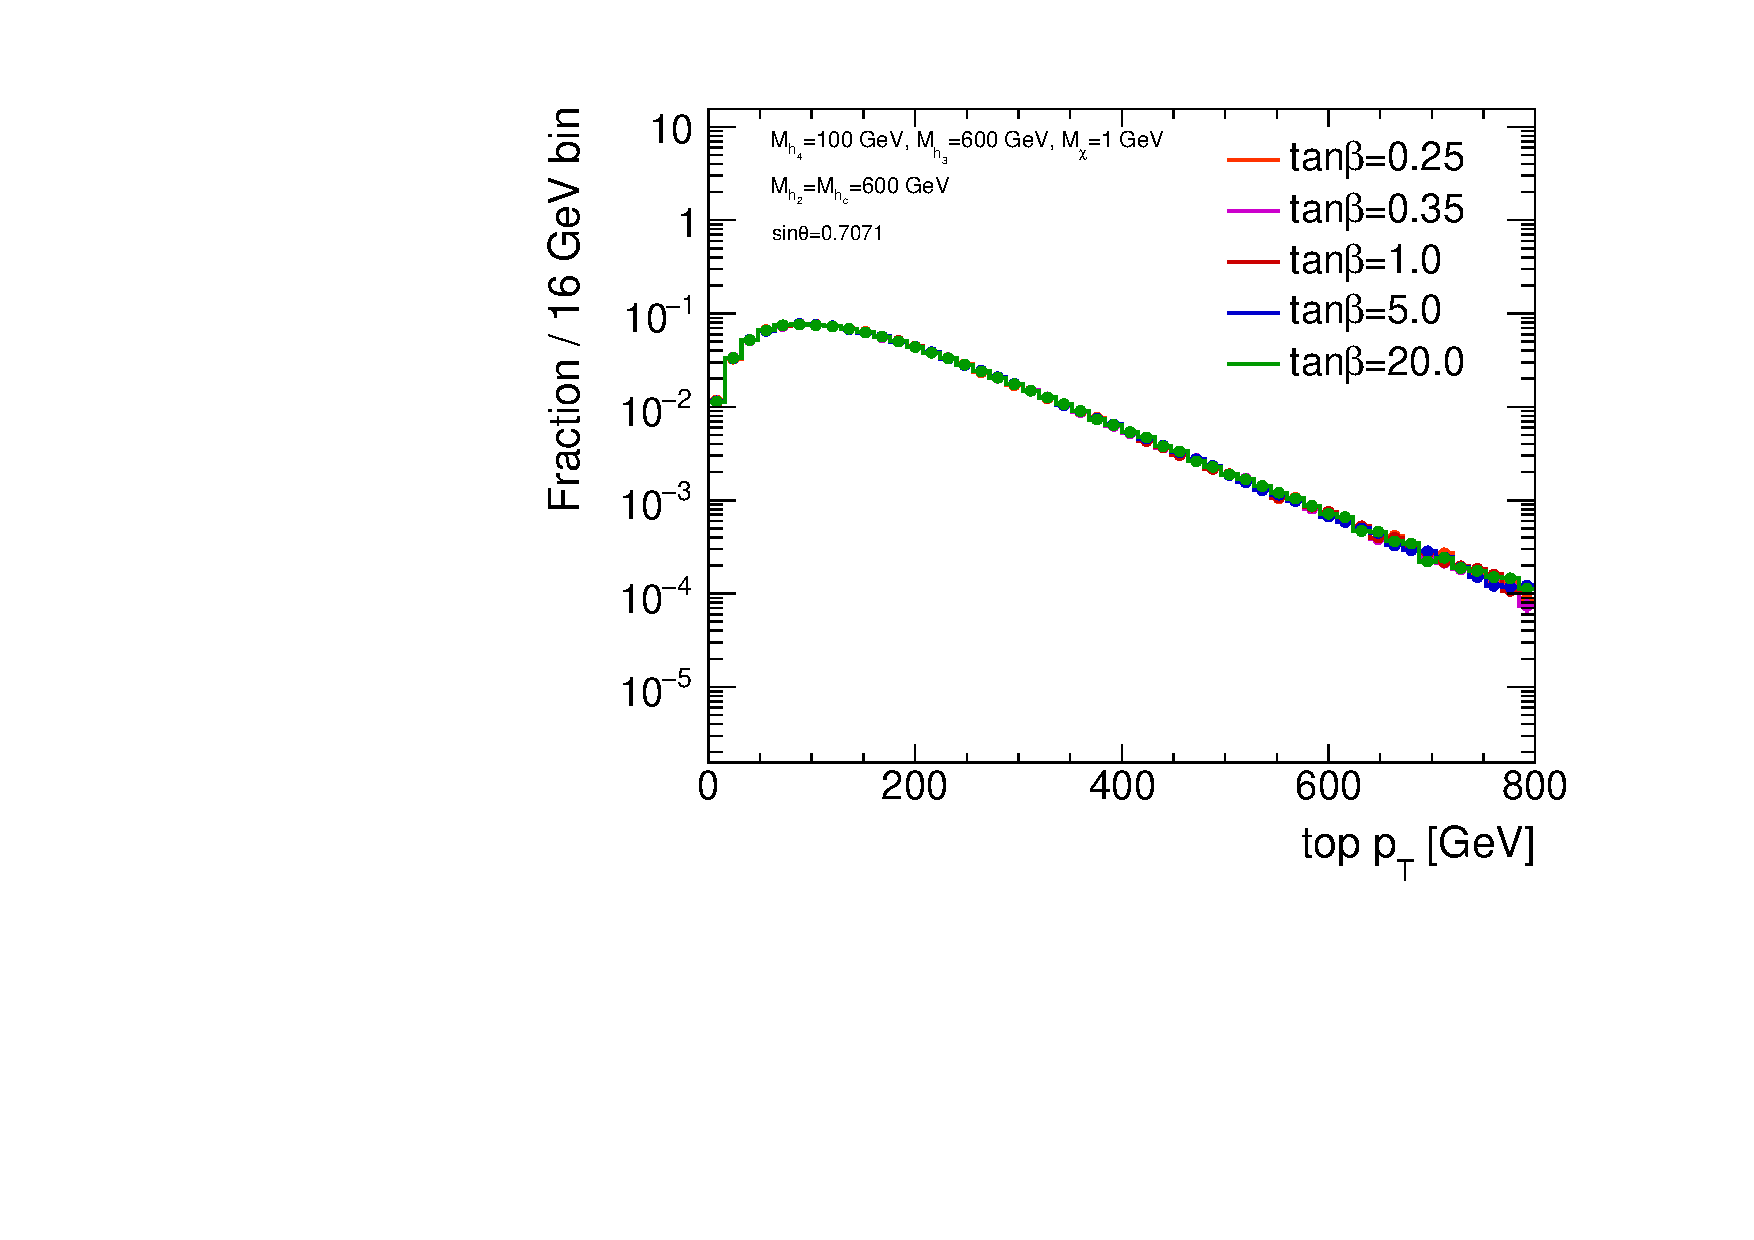
\includegraphics[width=\textwidth]{texinputs/04_grid/figures/DMHF/benchmarking/MDM_1_Ma_100_MA_600_sinp_0.7071_SCAN_tanb_decayed/topptlog.pdf}
    \caption{top $p_{T}$}
  \end{subfigure}
  \caption{The $E_{T}^{miss}$ and top $p_{T}$ distribution for inclusive $t\bar{t}+\chi\bar{\chi}$ production for various values of $\tan\beta$, with $\mathrm{M_a}=100$ GeV, $\mathrm{M_A}=600$ GeV, $\mathrm{M_H}=\mathrm{M_{H^{\pm}}}=600$ GeV, and $\sin\theta=0.7071$.}
  \label{fig:kin_tanB}
\end{figure}

In the $t\bar{t}$ + \MET signature, and in the limit of small $\tan\beta$ values, the couplings of $A$ ($h_{3}$ in the figure) and $a$ ($h_{4}$ in the figure) to down-type quarks are heavily suppressed regardless of the Yukawa assignment. At LO, $t\bar{t}+\chi\bar{\chi}$ associated production is mediated through either CP-odd weak eigenstate, $A$ or $a$, though it is shown in \autoref{fig:mchichi_tanB} that $a\rightarrow\chi\bar{\chi}$ is the dominant production mode. 
Although the relative mediator contribution is dependent on $\tan\beta$, observables such as $E_{T}^{miss}$ and top quark $p_{T}$ only have a moderate kinematic dependence on $\tan\beta$ as demonstrated in \autoref{fig:kin_tanB} before any analysis cuts. 
Other variables, such as the transverse mass $\MT$, are more affected by the contribution of the high mass mediator, as shown in \autoref{fig:kin_tanB} after kinematic cuts. 
For this reason, and since the production cross section times branching ratio for the $b\bar{b}$ + \MET signature is enhanced at high values of $\tan\beta$ (\textbf{Show cross-section plot when available}) \emph{it is desirable to perform a coarse scan in $\tan\beta$ as well}. 

It is interesting to note however that the relative total width for the heavy scalar $H$ becomes unphysically large at high $\tan\beta$ when all scalars have the same mass, due to the very large $H\rightarrow aa$ rate. 
%CD this is not clear for me what is the choice of a in this? 
This can be cured by tuning the mass of the heavy scalar so that the coupling between the heavy scalar and the light pseudoscalar $g_{Haa}$ becomes small for this scan only, therefore suppressing the $H\rightarrow aa$ rate that drives the width. An example of the heavy scalar width as a function of $\tan\beta$, with $\mathrm{M_H}=\mathrm{M_A}=600$ GeV, $\mathrm{M_{H^{\pm}}}=664$ GeV, $\sin\theta=0.35$, \mdm=10 GeV and \gdm=1 is shown in Fig.~\ref{fig:higgsWidth}. 

Even though this choice of parameters for this scan introduces a specific tuning and therefore model-dependence, it can be justified by noting that the trilinear scalar couplings are very sensitive to changes in the model's masses and couplings, and this in turn changes the decay partner of the heavy scalar and of the Higgs partners. Furthermore, the Higgs width does not influence the $b\bar{b}$ + \MET signal directly. Nevertheless, if this is tuning is not performed, particular care has to be taken at high $\tan\beta$ values to obtain reasonable results outside the narrow-width approximation, both for the generation of the signal and for the interpretation of the results.  

\begin{figure}
  \centering
  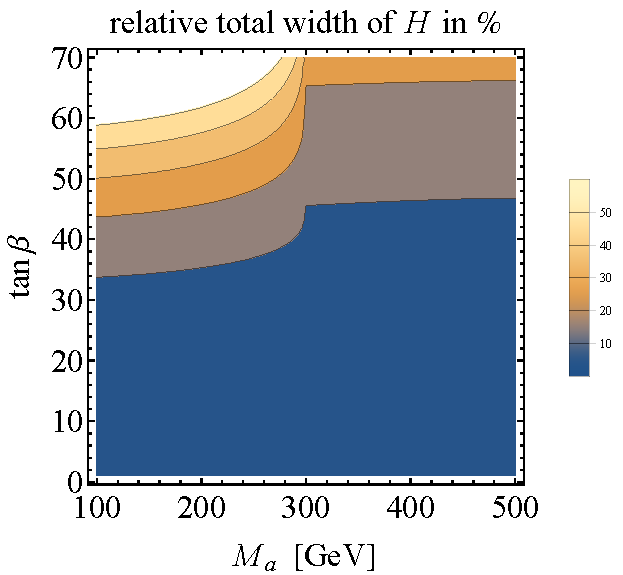
\includegraphics[width=0.7\textwidth]{texinputs/04_grid/figures/DMHF/benchmarking/Gamma5.pdf}
  \caption{The width of the heavy scalar as a function of $\tan\beta$, with $\mathrm{M_H}=\mathrm{M_A}=600$ GeV, $\mathrm{M_{H^{\pm}}}=664$ GeV, $\sin\theta=0.35$, \mdm=10 GeV and \gdm=1.}
  \label{fig:higgsWidth}
\end{figure}

%Dear all.
%
%I attach some plots that show the relative total widths for all scalars. 
%
%For Gamma1.pdf to Gamma4.pdf I used the parameters 
%
%M_H = M_A = M_H^+ = 600 GeV, 
%lambda_i = 3, i = 3, P1, P2
%g_DM = 1
%sin(theta) = 0.35
%m_DM = 10 GeV
%
%As you can see the widths of a, A  and H^+ are fine, but the one of H is not for 
%this choice of parameters. 
%
%The problem with the huge width of H can be "cured" by tuning M_H^+ so that 
%the coupling g_Haa as given in (4.9) of https://arxiv.org/pdf/1701.07427.pdf 
%becomes small thereby suppressing the H -> aa rate that drives Gamma(H) 
%large. 
%
%For instance for the above parameters taking 
%
%M_H = M_A  = 600 GeV
%
%but 
%
%M_H^+ = 664 GeV
%
%leads to the plot Gamma5.pdf. In this case tan(beta) can be taken to be 50 
%without running into trouble with the narrow-width approximation. 
%
%I am not sure if everybody is happy with this fix. I think it is fair to say that 
%the trilinear scalar couplings are rather model dependent, meaning that by 
%changing the masses M_j and couplings lambda_i one can change them 
%a lot which in turn will change the decay pattern of the Higgses. 
%
%Another point of view could be that one ignores that H has a huge width
%because it does not contribute to the bbbar + MET signal. 
%
%Best.
%
%Uli 
%


\begin{figure}[tbp]
\centering
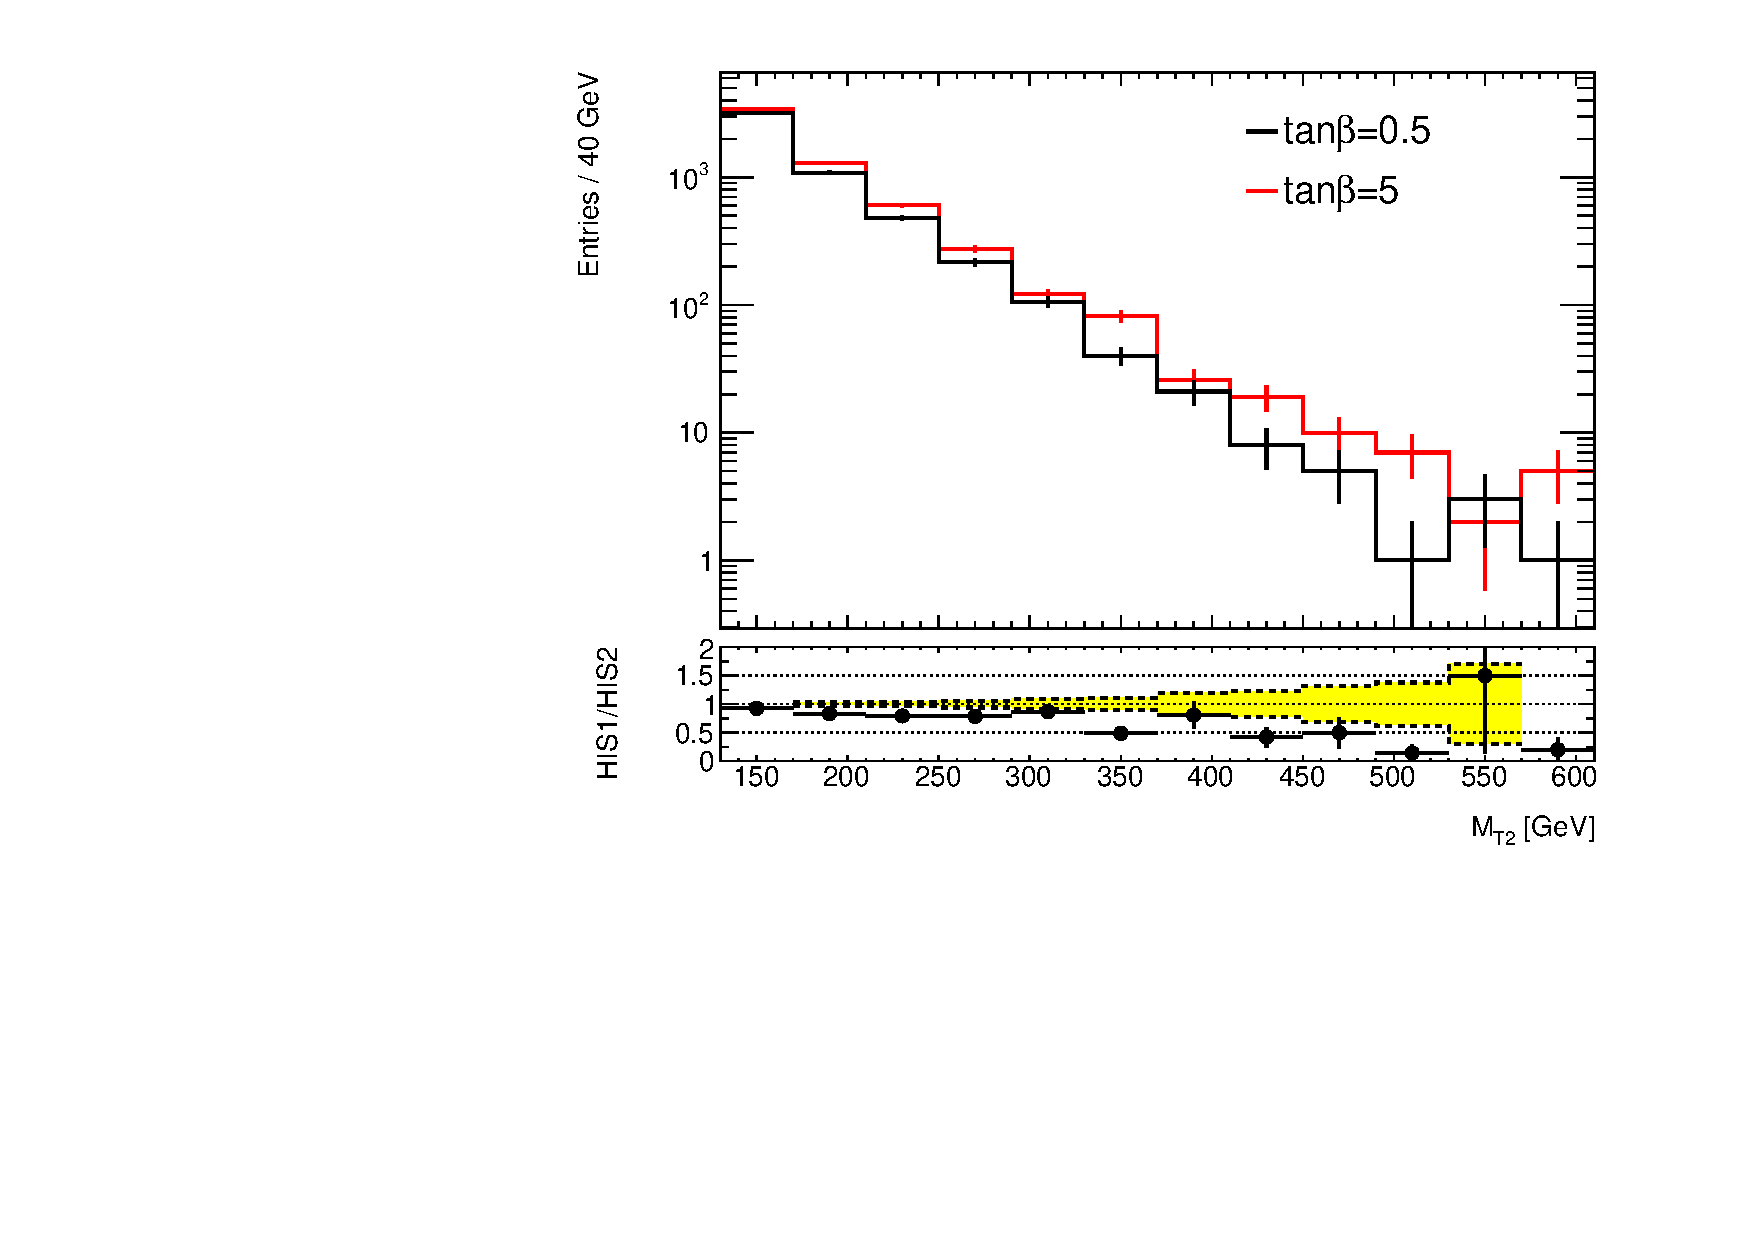
\includegraphics[width = 0.7\textwidth]{texinputs/04_grid/figures/DMHF/mt2plot_comparisonTanBeta.pdf}
  \caption{The $\MT$ distribution in the $t\bar{t}$ + \MET signature for different values of $\tan\beta$, after all selection cuts.\label{fig:kin_tanB_afterCuts}}
\end{figure}

%\subsubsection{Mass of DM fermion ($\mDM$)}
%
%The mass of the DM fermion $\mDM$ can change the total cross section and shape of the $\MET$ distribution, depending on the mass hierarchy of the $A,a,h,\chi$ particles. This is demonstrated in \autoref{fig:monoHbb_mDM_scan_met}. 
%Provided on-shell  decays $a\to\chi\chi$ are possible, i.e., $\mDM < \ma/2$, the exact value of \mDM has no effect on either kinematics or the total cross section. 
%The only exception is the case $\ma/2 > \mDM > \frac{1}{2}(\ma - M_h)$. In this  $\mDM$ range, the non-resonant process $a \to h A^*\left(\chi\chi\right) $ is kinematically inaccessible. 
%This reduces the overall cross section relative to the $\mDM \leq \frac{1}{2}(\ma - M_h)$ case, and slightly changes the soft part of the total $\MET$ spectrum. 
%However, since the contribution of the $a \to h A^*\left(\chi \chi\right)$ process is minor in any case, the differences are negligible.
%
%If the DM particle mass is exactly on threshold, i.e., $\mDM = \ma/2$, the total cross section is resonantly enhanced. 
%This resonant threshold enhancement drops rapidly towards both higher and lower $\mDM$. Furthermore, the shape of the $\MET$ distribution at threshold, where amplitudes involving $a\to\chi\chi$ decays make up a larger fraction of the signal, differs significantly from the one below threshold. 
%Below threshold ($\mDM > \ma/2$), the total cross section quickly drops by several orders of magnitude. In this regime, the shape of the $\MET$ distribution changes with $\mDM$ continuously.
%
%\begin{figure}[tbp]
%\centering
%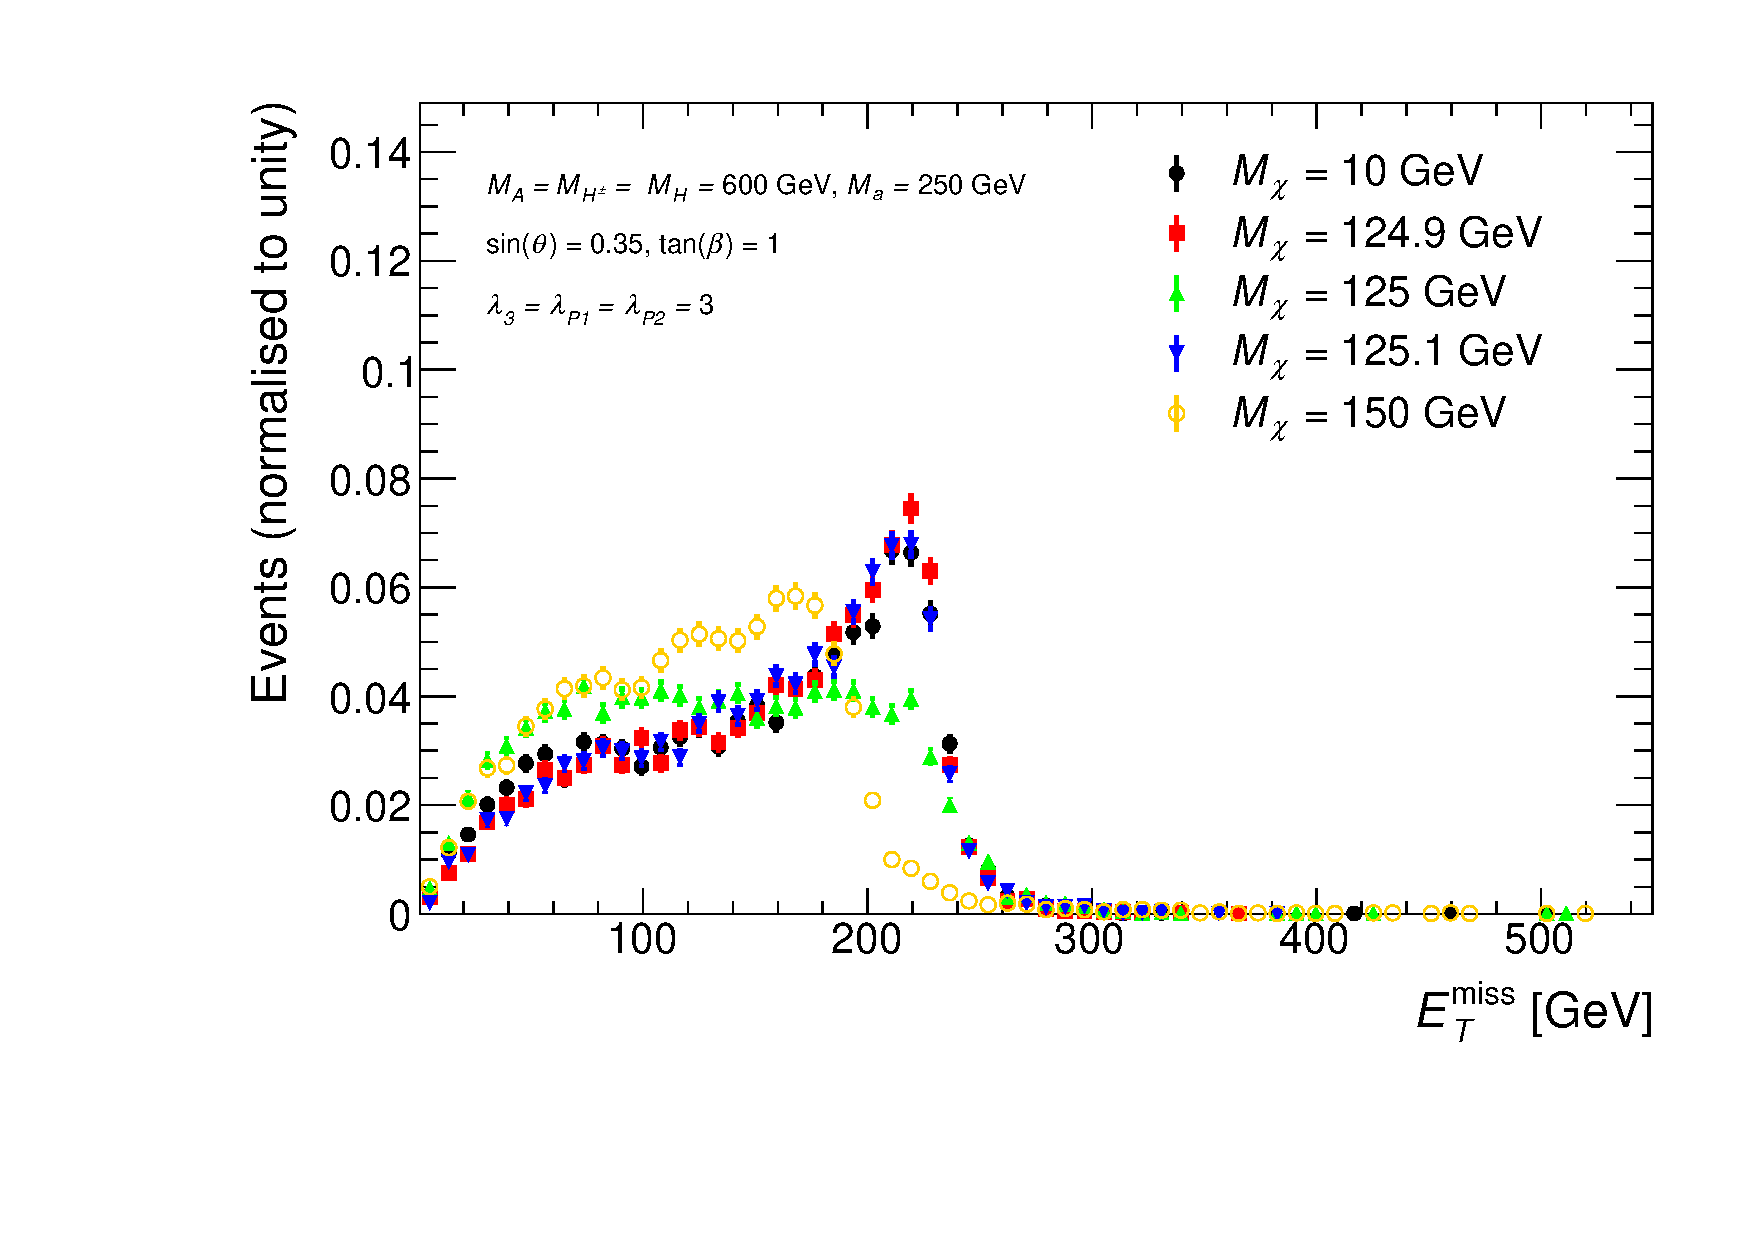
\includegraphics[width=0.7\textwidth]{texinputs/04_grid/figures/monoHbb_mDM_scan_MET_liny_norm2one.pdf}
%\caption[$\MET$ distribution in \monohbb events for different $\mDM$]
%{
%Missing transverse momentum distribution  of \monohbb signal events at parton level for five representative models with different $\mDM$
%and fixed $\mA = \mH = \mHc = 600 $ GeV $\ma = 250$ GeV, $ \sinp = 0.35, \tanb = 1$ and $ \lap1 = \lap2 = \lam3 = 3 $. 
%The shape of the $\MET$ distribution does not change for $\mDM < \ma/2$, then changes significantly for $\mDM>=\ma/2$.
%\label{fig:monoHbb_mDM_scan_met}
%}
%\end{figure}
%
%Similar effects are seen in \autoref{fig:dm_scan_ll}. In the $\mDM < \frac{\ma}{2}$ region, \mDM has no effect on event yield or \MET distribution, at $\mDM = \frac{\ma}{2}$ a resonant enhancement to the cross section occurs, and in the off-shell region where  $\mDM > \frac{\ma}{2}$ cross section steeply drops.  The \MET shape remains the same up to, and even slightly above, $\mDM = \frac{\ma}{2}$, but further off shell the \MET distribution becomes increasingly disperse.  For \mDM = 200 \GeV, DM can still decay on-shell through the $A$.  For \mDM = 500 \GeV both pseudoscalars are off-shell leading to an event yield too low to fit on the figure on the left and a \MET distribution without structure.
%
%\begin{figure}
%\centering
%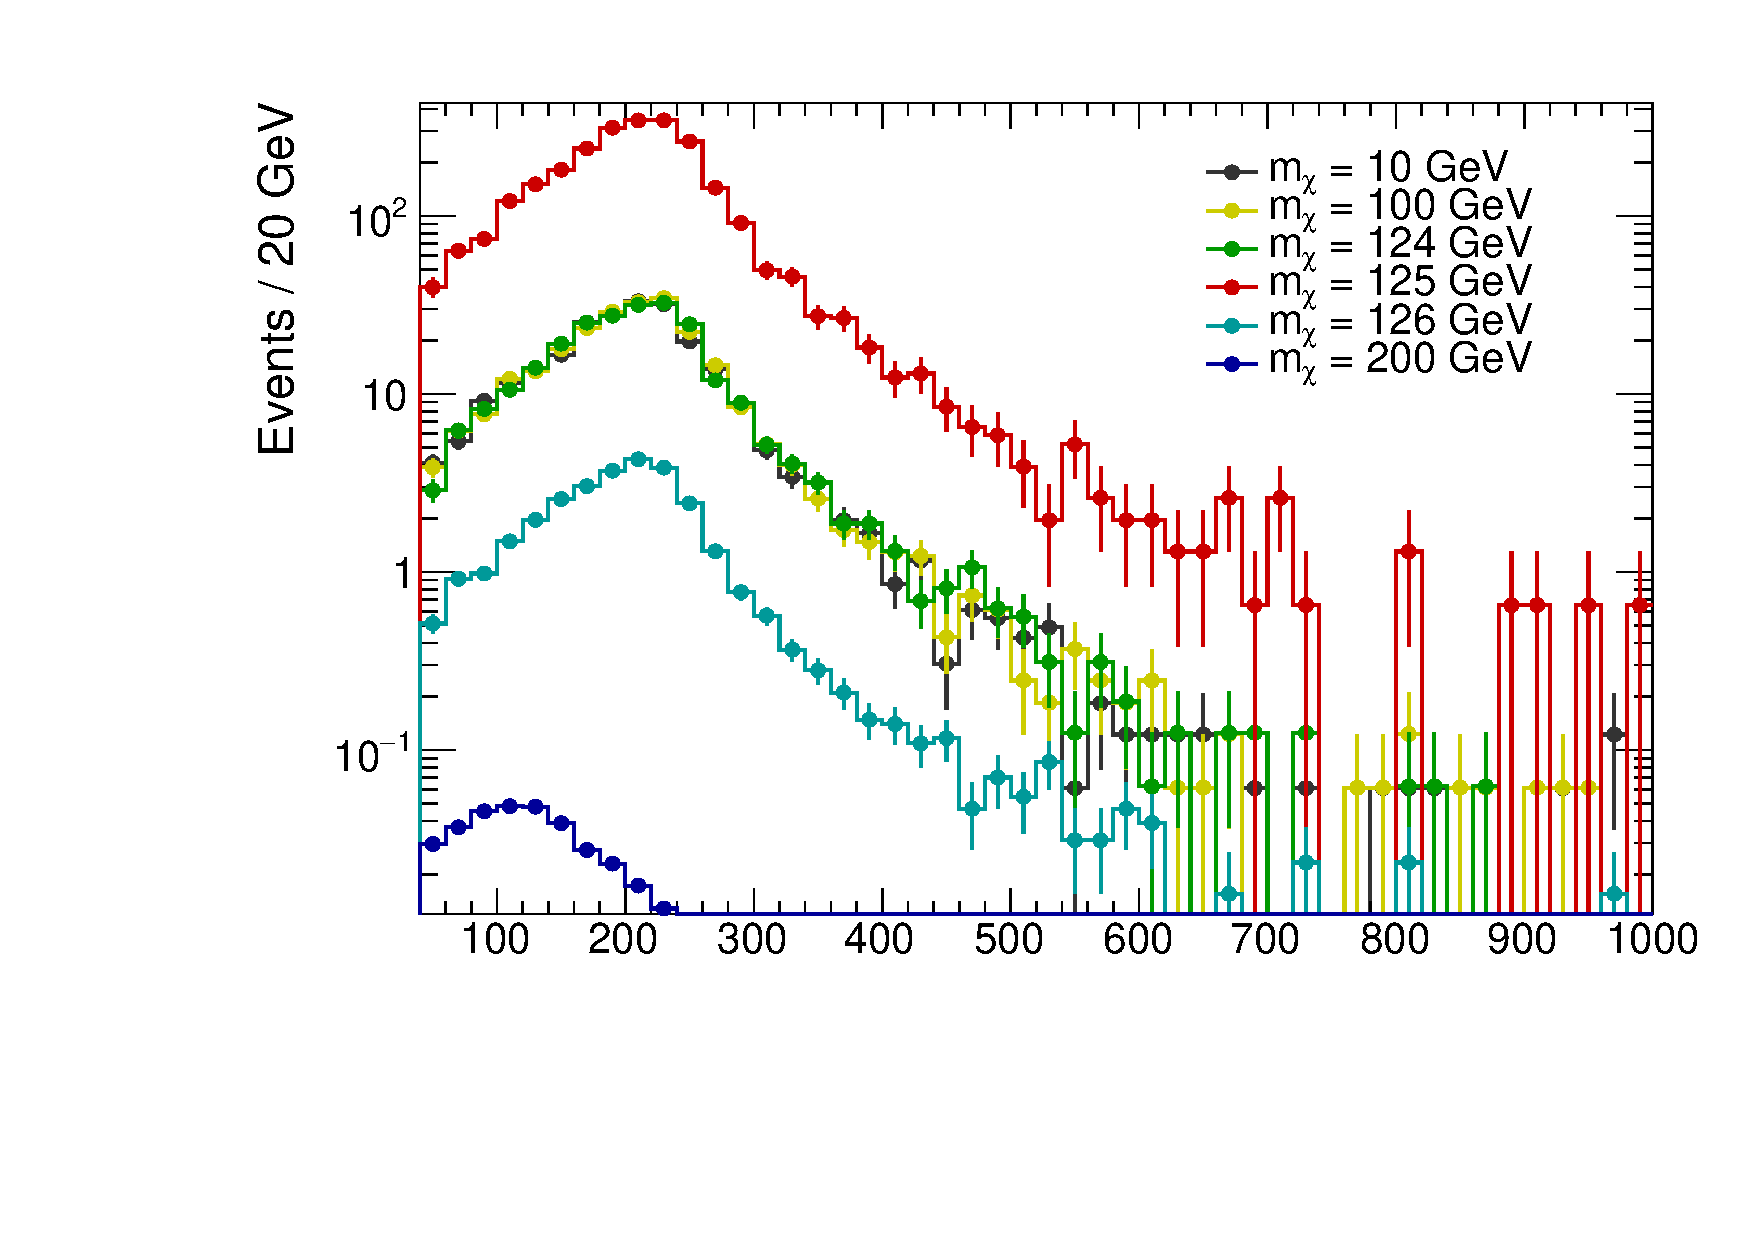
\includegraphics[width=0.48\textwidth]{texinputs/04_grid/figures/monoz/leptonic/mDMScan_mA600_ma250_MET.pdf}
%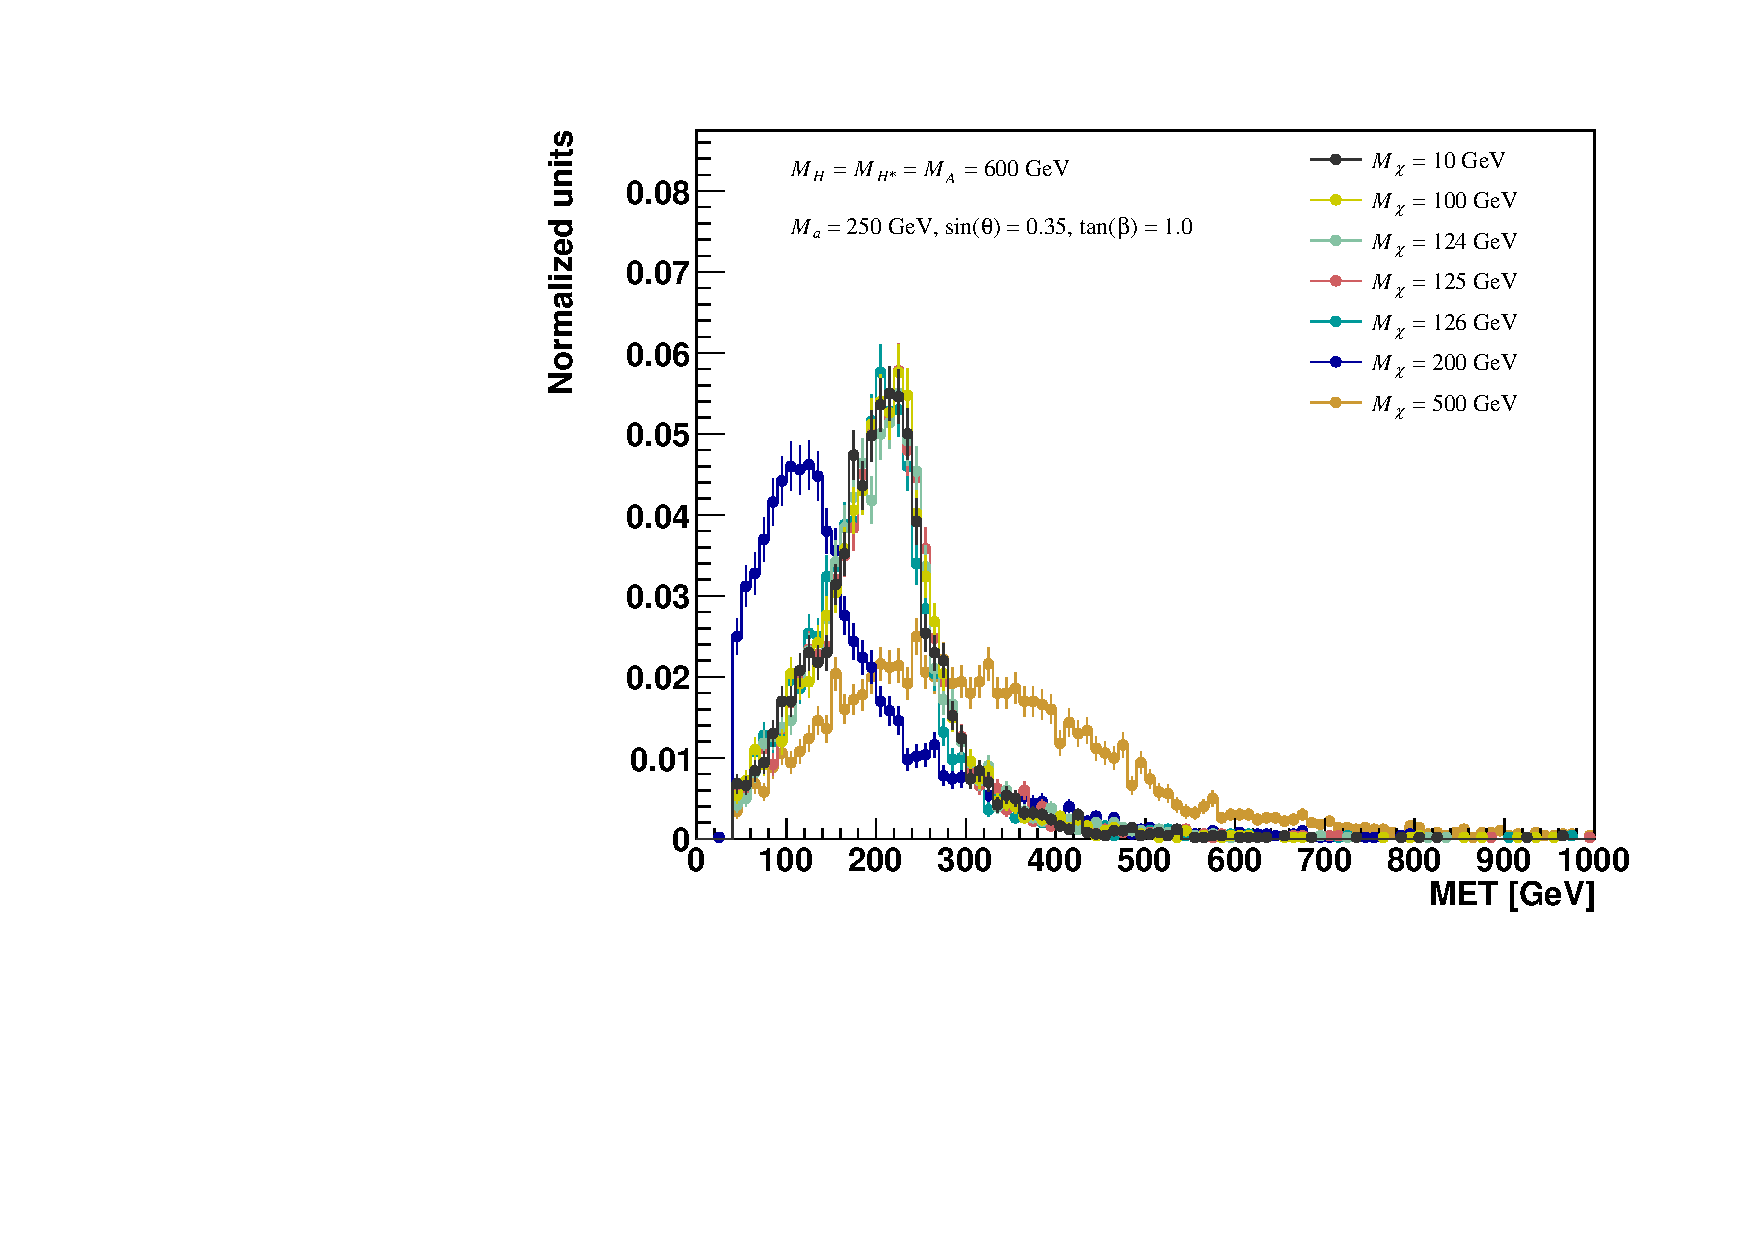
\includegraphics[width=0.47\textwidth]{texinputs/04_grid/figures/monoz/leptonic/mDMscan_ma250.pdf}
%\caption{\MET distributions following preselection in the Z(lep) +\MET search are shown (left) scaled to 40 \ifb and (right) normalized to unity for different values of \mDM with fixed \mA = 600 \GeV and \ma = 250 \GeV.}
%\label{fig:dm_scan_ll}
%\end{figure}
%
%A value of $\mDM$=10 is chosen for the following studies, as it produces a cross-section that is sufficiently large for this model to be detected with Run-2 LHC data and highlights the resonant features of the \MET spectrum.
%%TODO: mention instability
